We evaluated \textbf{L-ISR-PHE} using seismic wave propagation, cosmology, and proxy ECP hydrodynamics simulations~(Section~\ref{sec:datasets}) for two aspects: (1) \textit{in situ} encumbrance under varying workloads~(Section~\ref{sec:results_insitu}); and (2) \textit{post hoc} efficacy for various configurations~(Section~\ref{sec:results_posthoc}).
%\begin{figure}[t]
\centering
%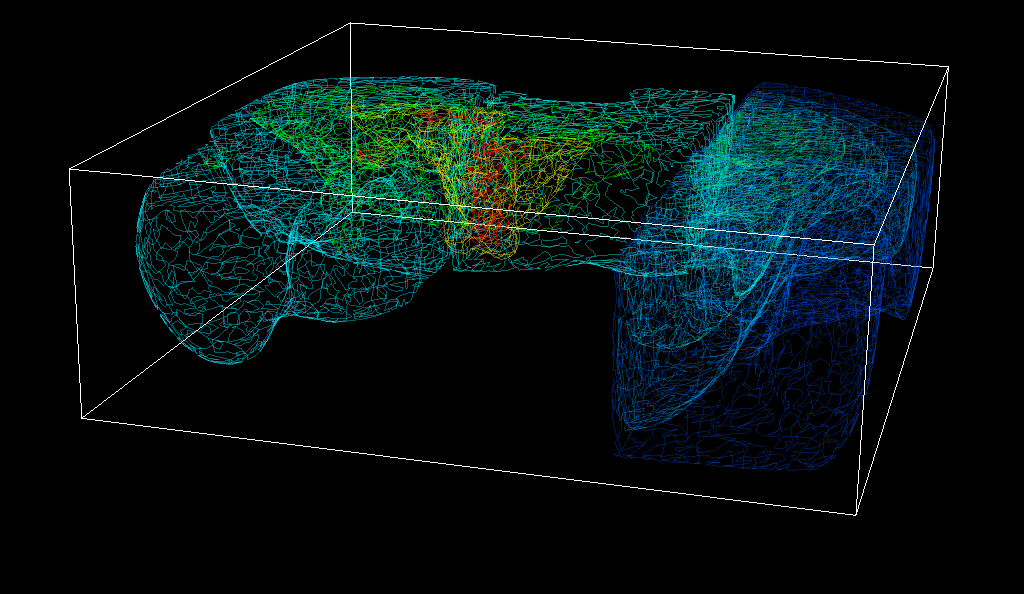
\includegraphics[width=0.8\linewidth]{images/sw4_vis_2.png}
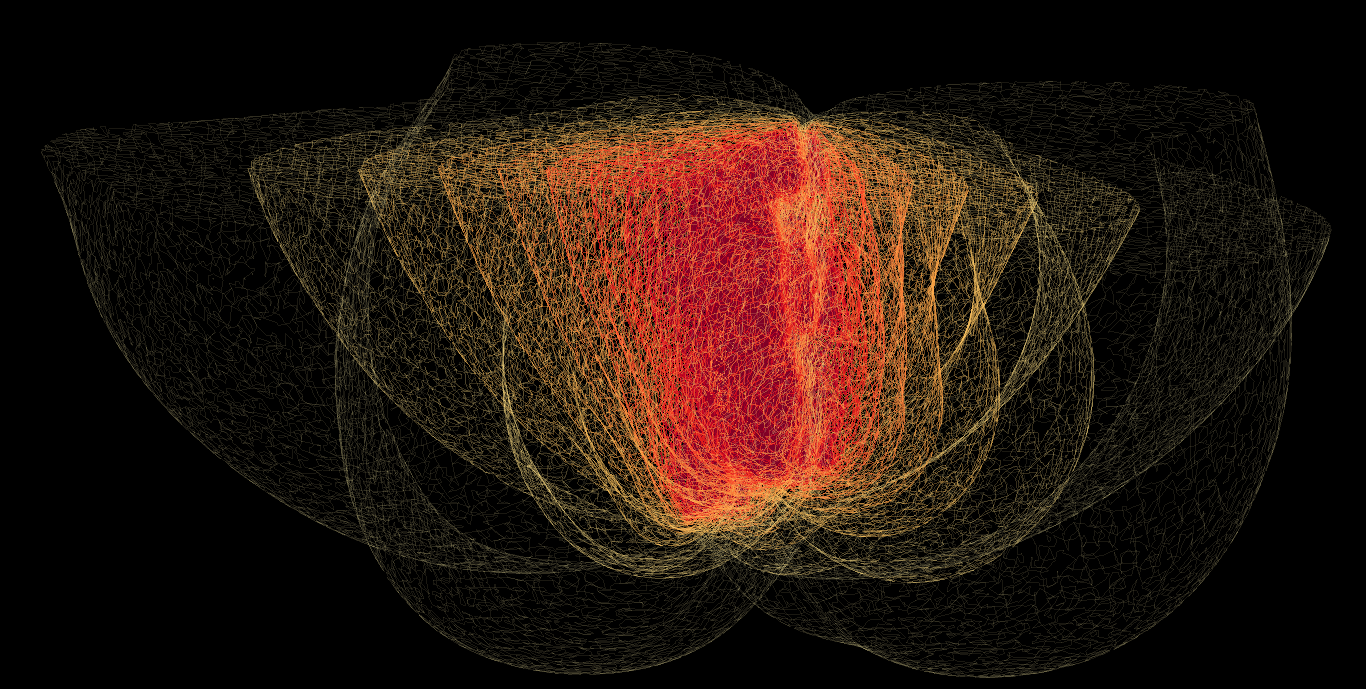
\includegraphics[width=0.8\linewidth]{images/sw4_waves.png}
\caption{SW4 wave propagation visualization}
\label{fig:sw4_vis}
\end{figure}



%\begin{figure}[t]
\centering
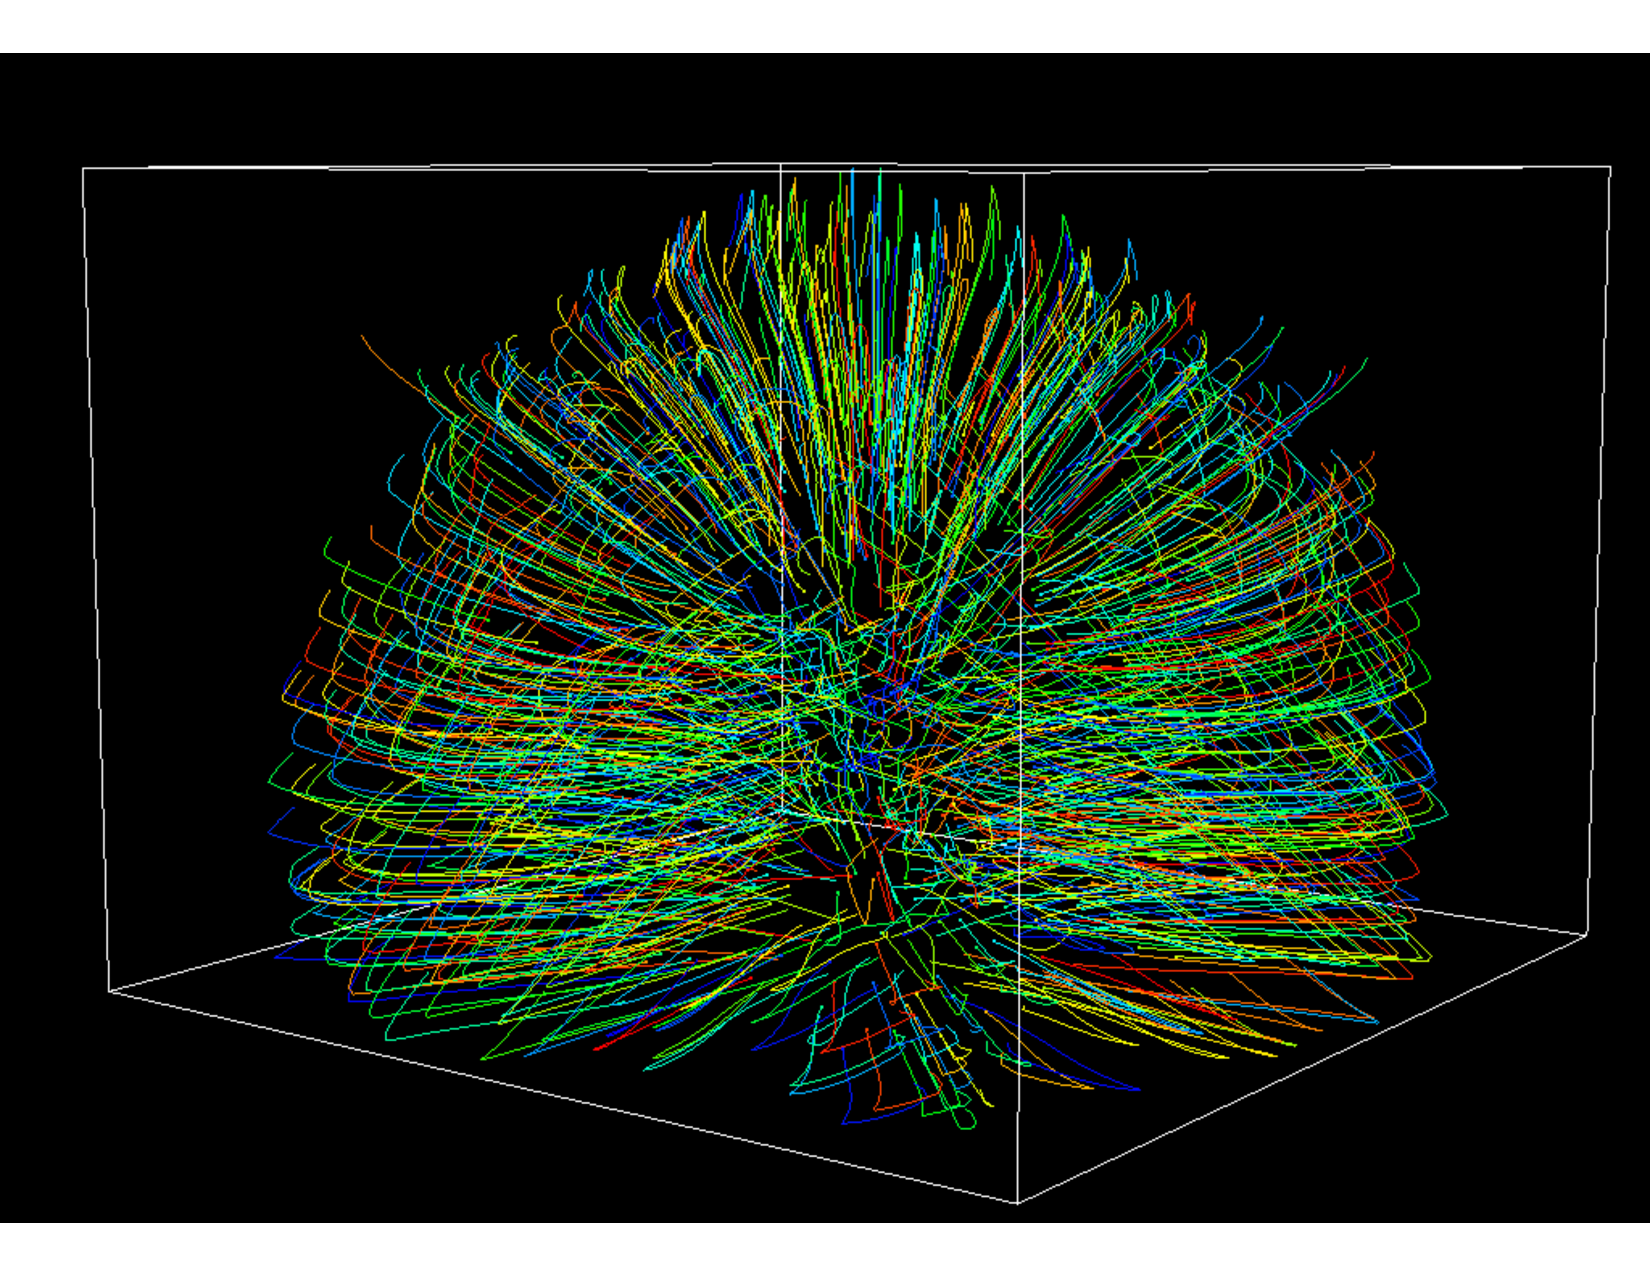
\includegraphics[width=0.7\linewidth]{images/pathlines_clover.pdf}
\caption{Cloverleaf3D flow visualization}
\label{fig:pathlines_clover}
\end{figure}



\begingroup
\setlength{\tabcolsep}{-2pt}
%\renewcommand{\arraystretch}{1} % Default value: 1
\begin{table*}[!h]
%\centering
\begin{tabular}{|P{1.1cm}|P{1.1cm}|P{2.7cm}|P{1.3cm}|P{1.3cm}|P{1.5cm}|P{2cm}  N  R|P{6cm}|}
\hline
Nodes & MPI & Dimensions & Interval & Sim$_{cycle}$ & Particles & Memory & Step & DAV\% & Scatter Plots\\ 
 & Ranks & & & & /Node & /Node (MB) & & & \\ 
\hline
%\multicolumn{9}{l}{} & \\
\multicolumn{9}{l}{\textbf{          Cloverleaf3D Proxy Hydrodynamics Application }} & \multirow{13}{*}{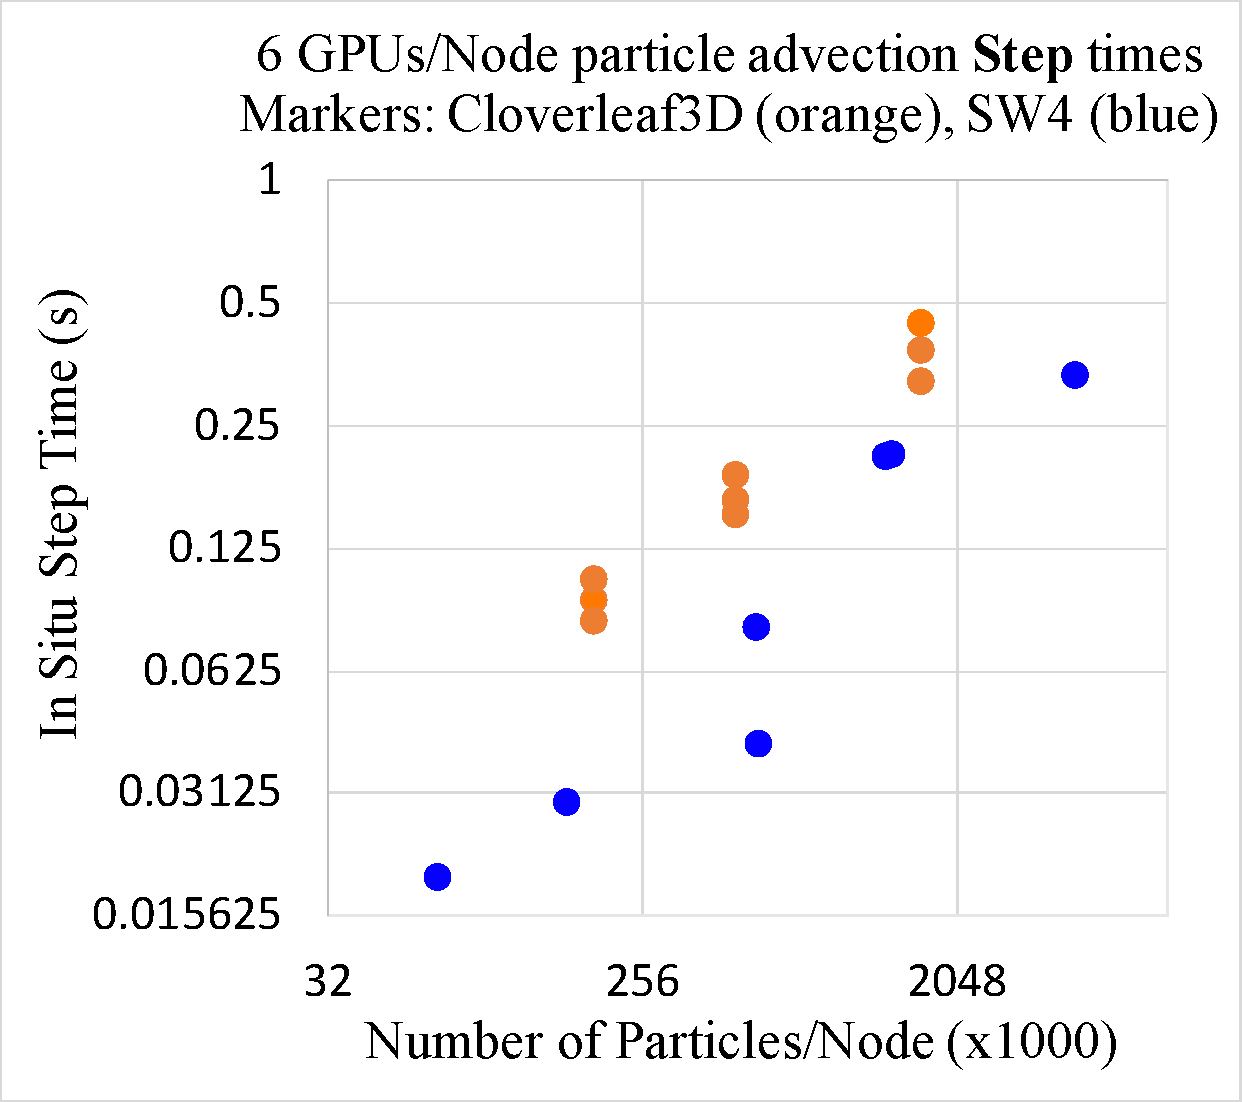
\includegraphics[width=0.93\linewidth]{images/GPU_Step.pdf}}\\
\cline{1-9}
\multirow{9}{*}{16} & \multirow{9}{*}{96} & \multirow{9}{*}{$586\times586\times586$} & 20 & 4.73 & \multirow{3}{*}{1.5M} & \multirow{3}{*}{40.2 } & 0.4475 & 9.408 & \\
\cline{4-4}
& & & 40 & 4.08 & & & 0.3221 & 7.894 & \\
\cline{4-4}
& & & 60 & 4.39 & & & 0.3838 & 8.742 & \\
\cline{4-6}%\cline{6-6}
& & & 20 & 4.50 & \multirow{3}{*}{474k} & \multirow{3}{*}{12 } & 0.1882 & 4.182 & \\
\cline{4-4}
& & & 40 & 4.14 & & & 0.1628 & 3.932 & \\
\cline{4-4}
& & & 60 & 4.33 & & & 0.1498 & 3.459 & \\
\cline{4-6}%\cline{6-6}
& & & 20 & 4.19 & \multirow{3}{*}{186k} & \multirow{3}{*}{4.2 } & 0.0925 & 2.207 & \\
\cline{4-4}
& & & 40 & 4.11 & & & 0.1043 & 2.537 & \\
\cline{4-4}
& & & 60 & 3.87 & & & 0.0830 & 2.144 & \\
\cline{1-9}
%\multicolumn{9}{l}{} & \\
\multicolumn{9}{l}{\textbf{          SW4 Seismic Modeling Simulation }} & \\
\cline{1-9}
\multirow{3}{*}{1} & \multirow{3}{*}{6} & $251\times251\times70$ & \multirow{7}{*}{200} & 0.35 & 555k & 13.89 & 0.0412 & 11.67 & \\
\cline{3-3}\cline{5-6}
& & $335\times335\times93$ & & 2.02 & 1.3M & 33.16 & 0.2125 & 10.48 & \\
\cline{3-3}\cline{5-6}  
& & $501\times501\times139$ & & 7.58 & 4.4M & 111.13 & 0.3309 & 4.365 & \multirow{13}{*}{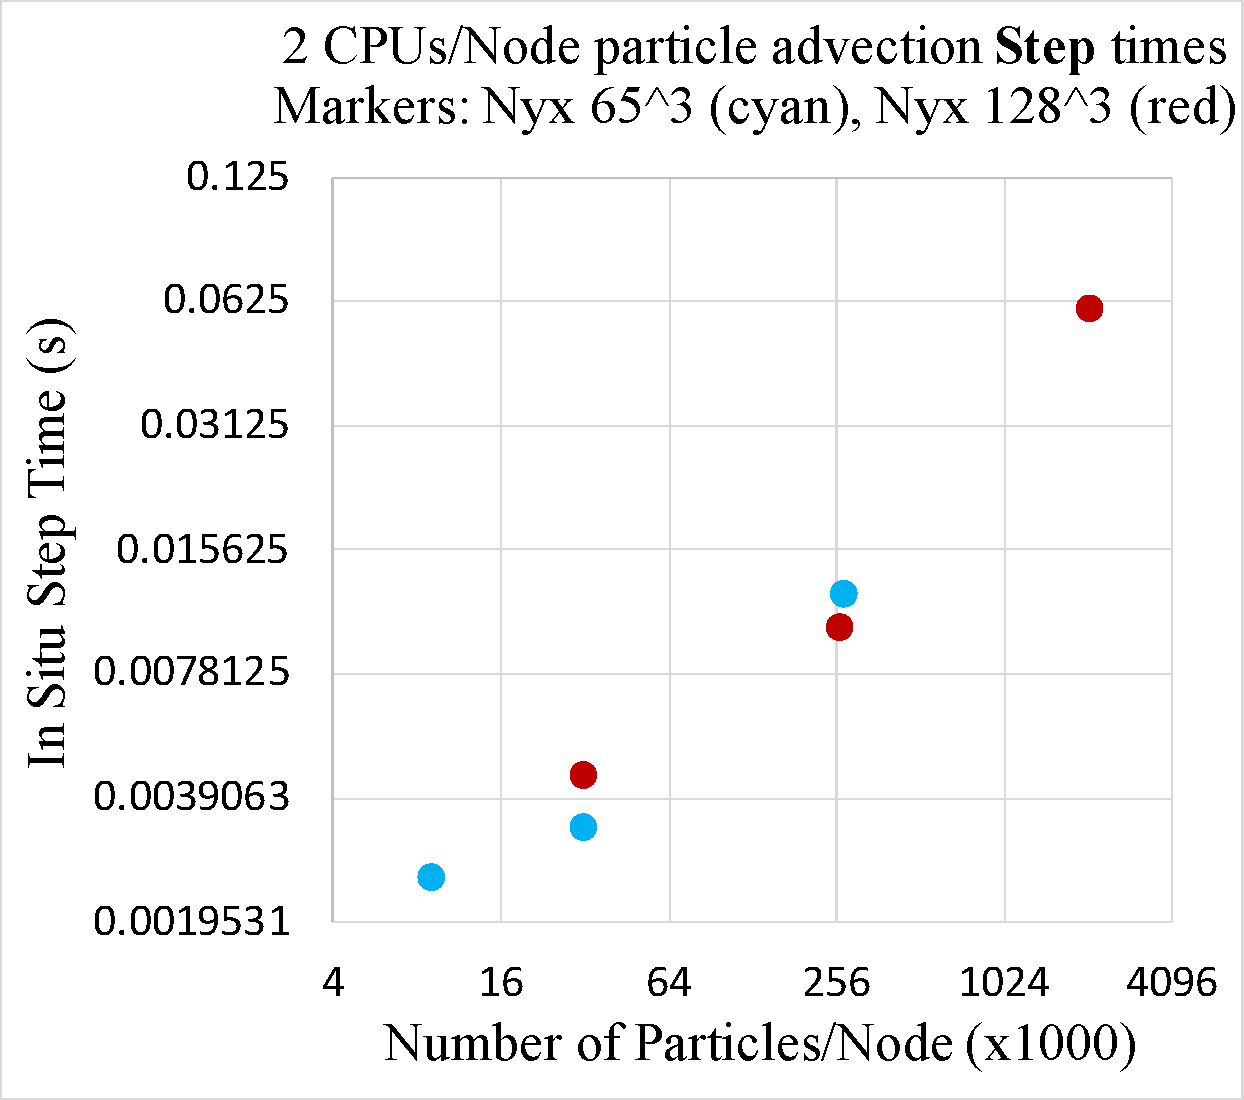
\includegraphics[width=0.93\linewidth]{images/CPU_Step.pdf}}\\
\cline{1-3}\cline{5-6}
\multirow{4}{*}{64} & \multirow{4}{*}{384} & \multirow{3}{*}{$1001\times1001\times276$} & & 1.6 & 66k & 1.6 & 0.0194 & 1.201 &  \\
\cline{6-6}
& & & & 1.5 & 146k & 3.6 & 0.0295 & 1.944 & \\
\cline{6-6}
& & & & 1.3 & 540k & 13.5 & 0.0798 & 6.175 & \\
\cline{3-3}\cline{5-6}
& & $1335\times1335\times368$ & & 2.9 & 1.2M & 31.9 & 0.2095 & 7.074 & \\
\cline{1-9}
%\multicolumn{9}{l}{} & \\
\multicolumn{9}{l}{\textbf{          Nyx Cosmology Simulation }} & \\
\cline{1-9}
\multirow{6}{*}{1} & \multirow{6}{*}{1} & \multirow{3}{*}{$65\times65\times65$} & \multirow{6}{*}{100} & \multirow{3}{*}{10.9} & 274k & 6.8 & 0.0122 & 0.112 & \\
\cline{6-6}
& & & & & 32k & 0.8 & 0.0033 & 0.030 & \\
\cline{6-6}
& & & & & 9k & 0.2 & 0.0025 & 0.023 & \\
\cline{3-3}\cline{5-6}
& & \multirow{3}{*}{$129\times129\times129$} & & \multirow{3}{*}{88.3} & 2.1M & 53.6 & 0.0596 & 0.067 & \\
\cline{6-6}
& & & & & 262k & 6.5 & 0.0101 & 0.011 & \\
\cline{6-6}
& & & & & 32k & 0.8 & 0.0044 & 0.005 & \\
\hline
\end{tabular}
\vspace{-3mm}
\caption{\textit{In situ} encumbrance evaluation and experiment configurations for our three simulation codes.}
\label{table:encumbrance}
\vspace{-5mm}
\end{table*}
\endgroup


\subsection{In Situ Encumbrance}
\label{sec:results_insitu}
%\begin{figure*}
\begin{subfigure}{0.195\textwidth}
\centering
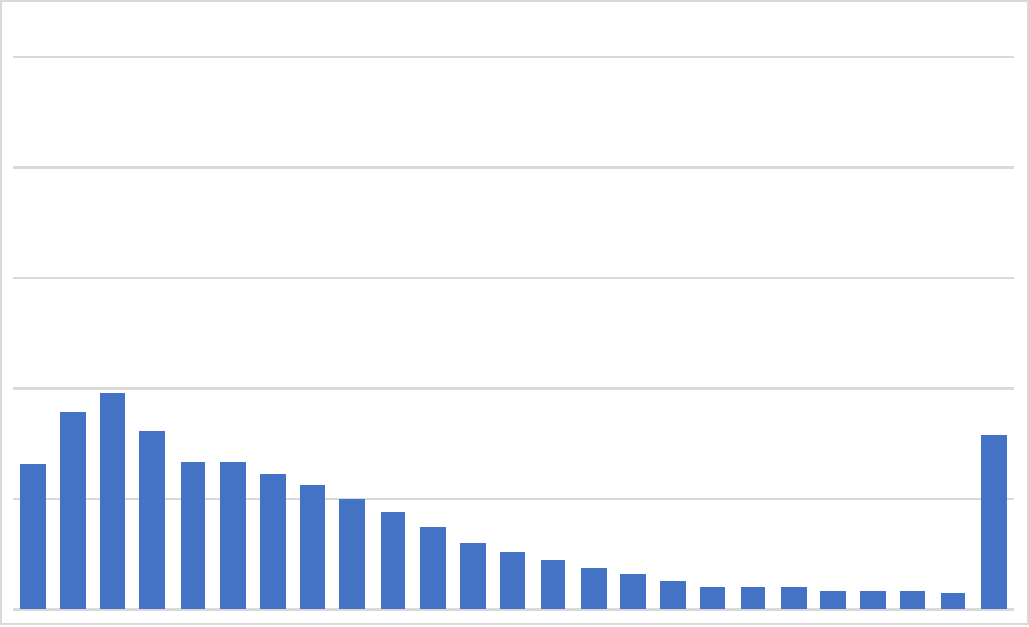
\includegraphics[width=0.9\linewidth]{results/cloverleaf3d/eul_1/Eul1_AvgL2.pdf}
\vspace{-2mm}
\caption{Eul 20 Avg$_{L2}$ L2 }
\end{subfigure}
\begin{subfigure}{0.195\textwidth}
\centering
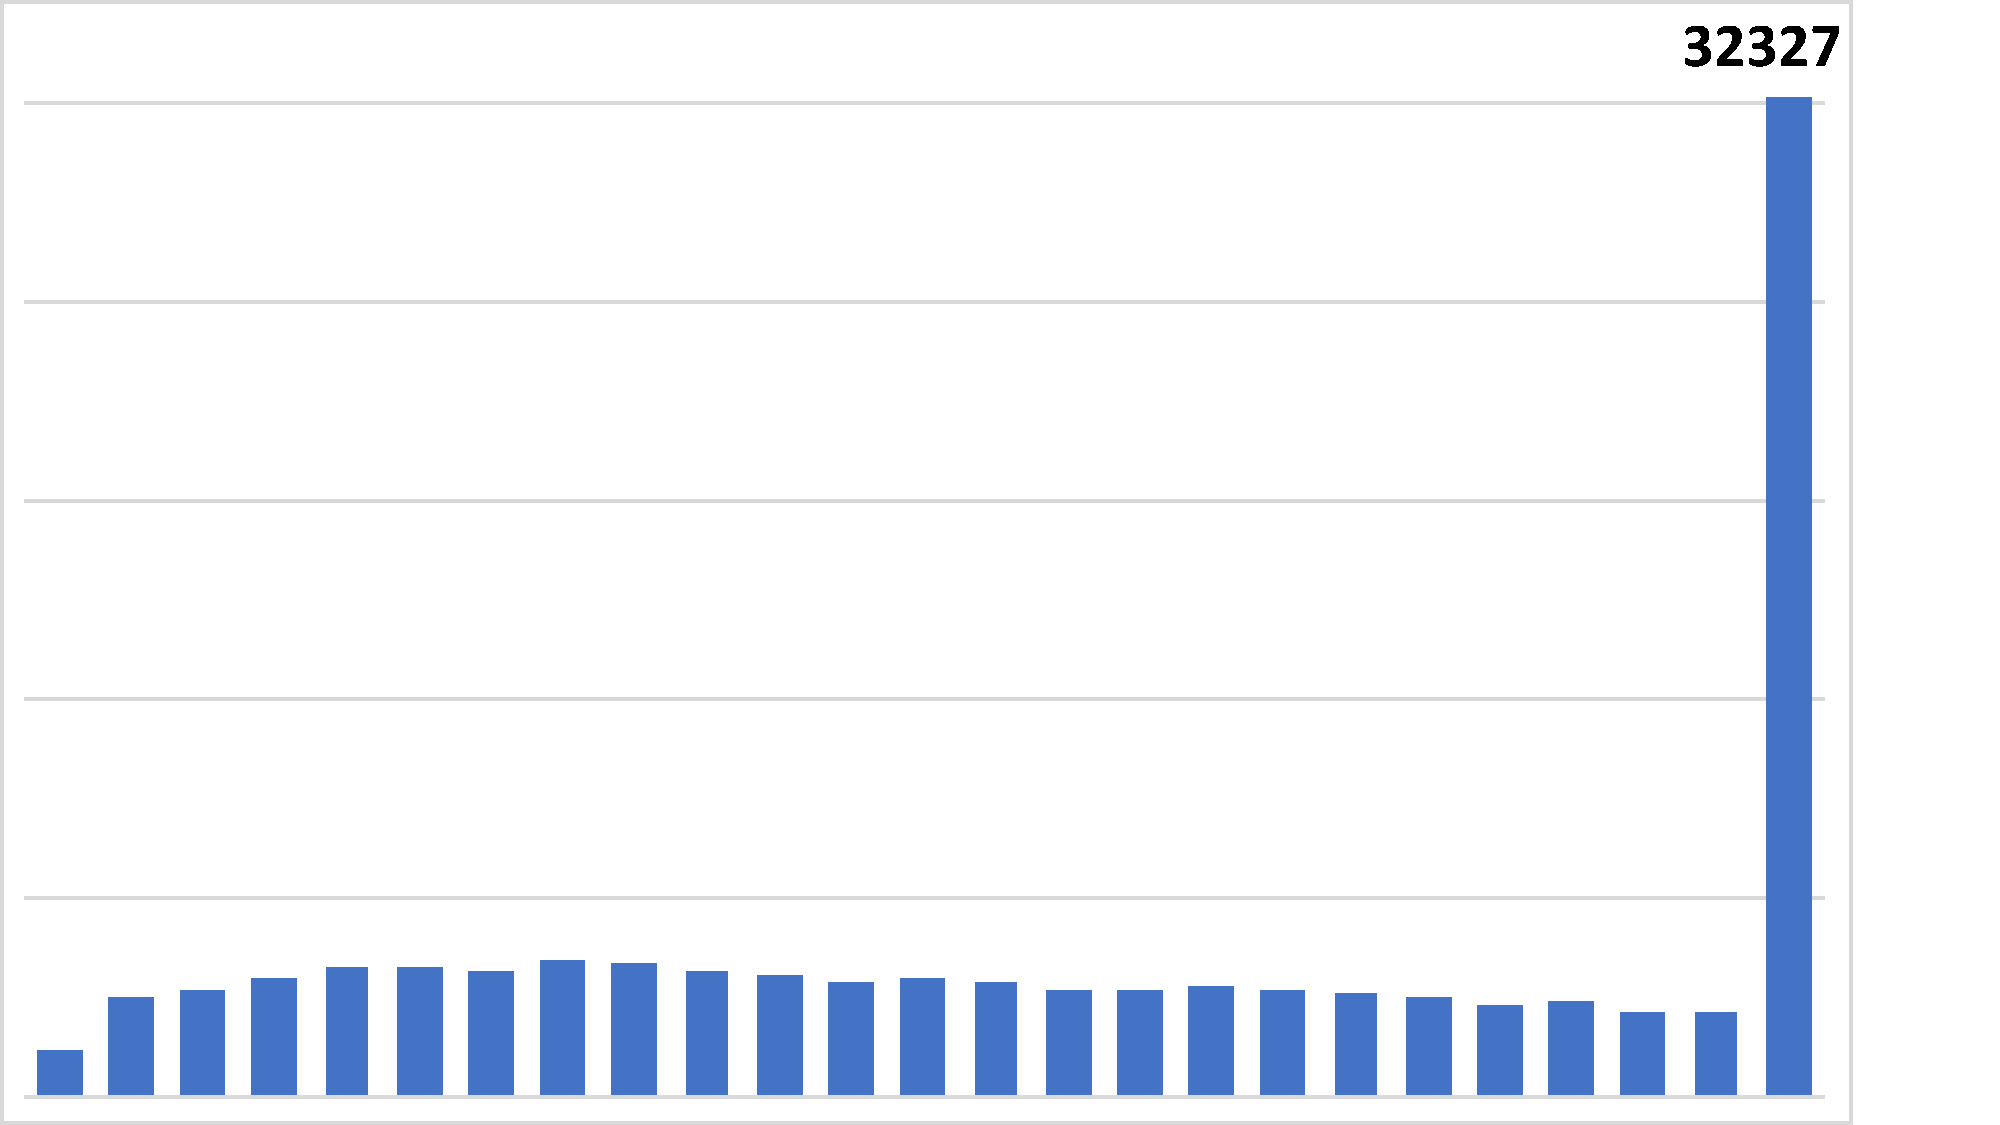
\includegraphics[width=0.95\linewidth]{results/cloverleaf3d/eul_2/Eul2_AvgL2.pdf}
\vspace{-2mm}
\caption{Eul 40 Avg$_{L2}$ L2 }
\end{subfigure}
\begin{subfigure}{0.195\textwidth}
\centering
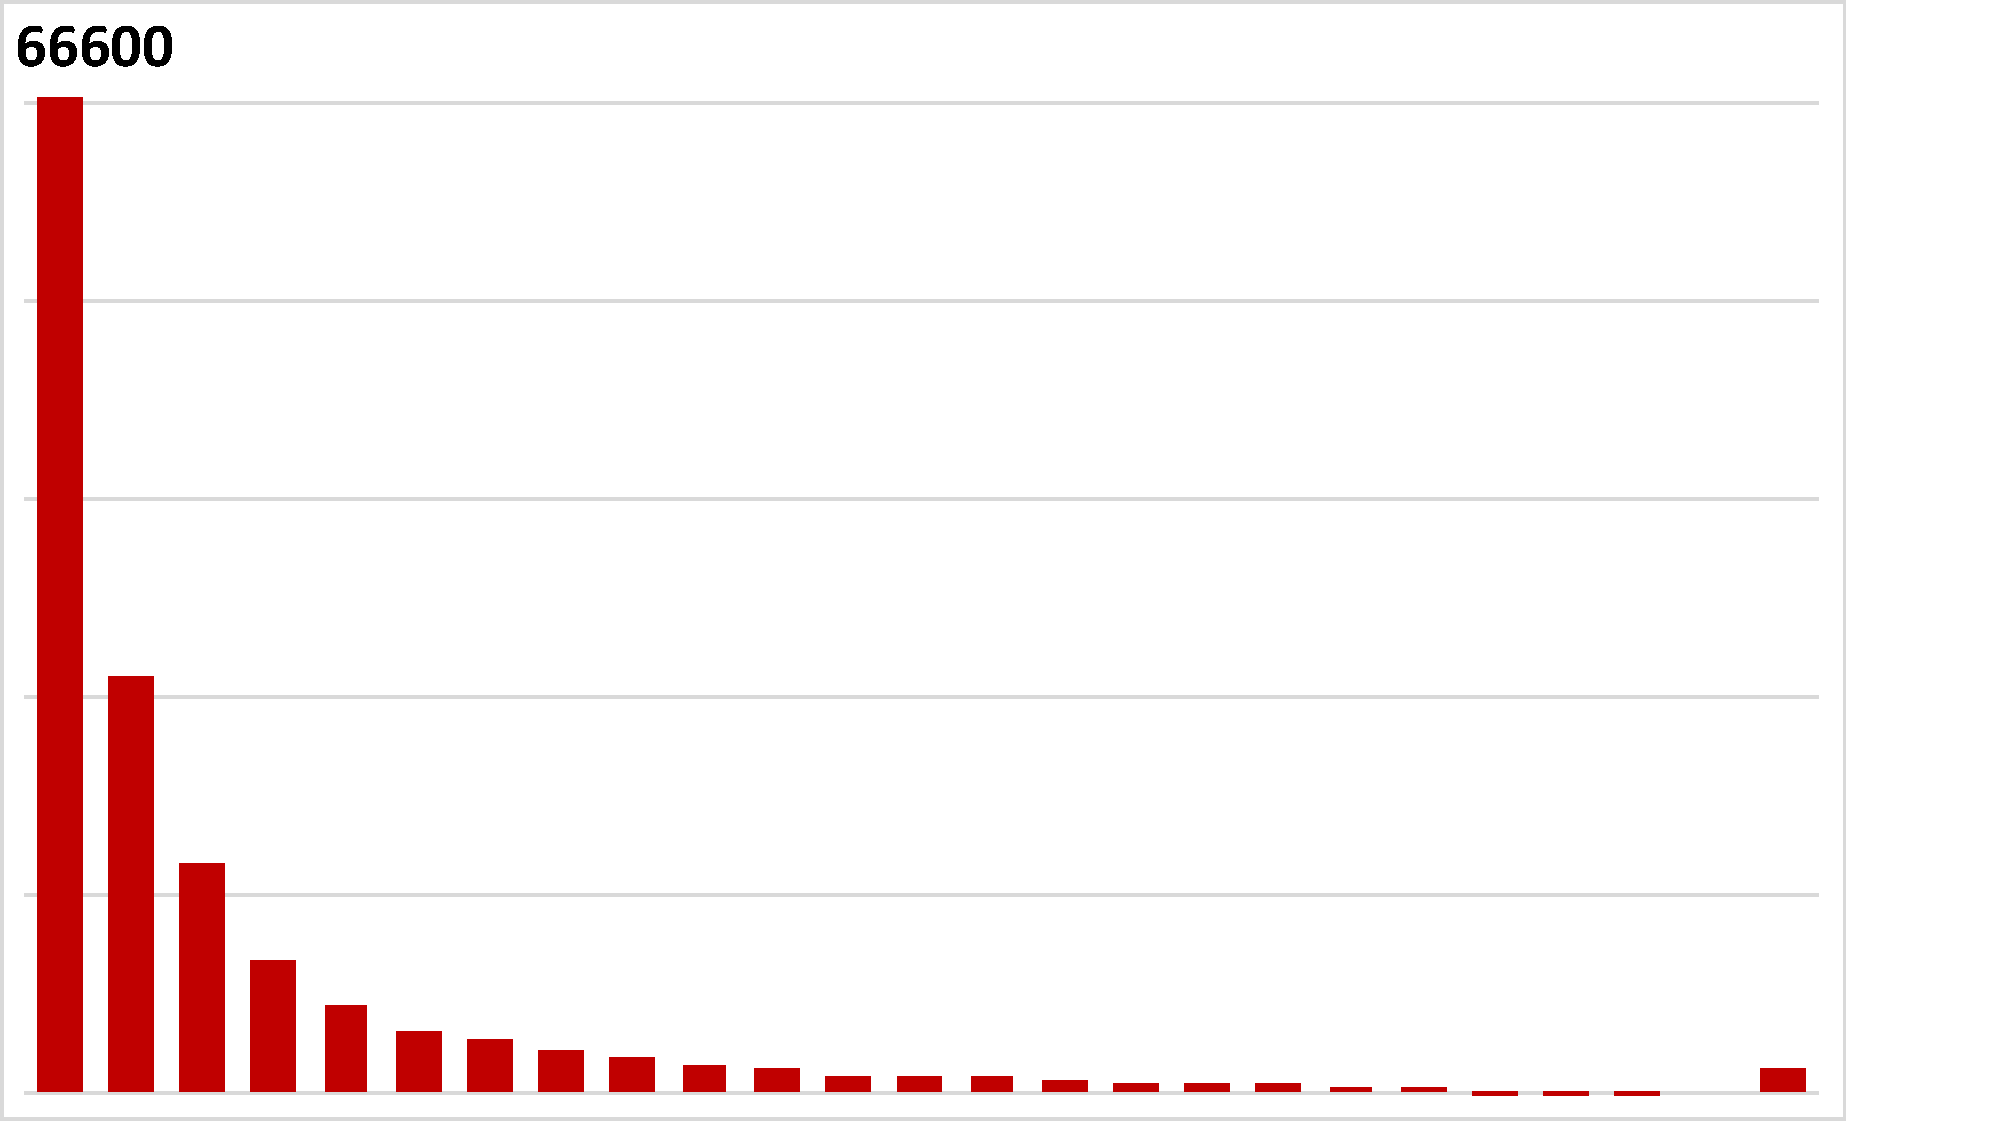
\includegraphics[width=0.9\linewidth, trim={0cm 0cm 2.5cm 0cm}, clip]{results/cloverleaf3d/lag_4/Lag4_AvgL2.pdf}
\vspace{-2mm}
\caption{Lag 40 1:8 Avg$_{L2}$ }
\end{subfigure}
\begin{subfigure}{0.195\textwidth}
\centering
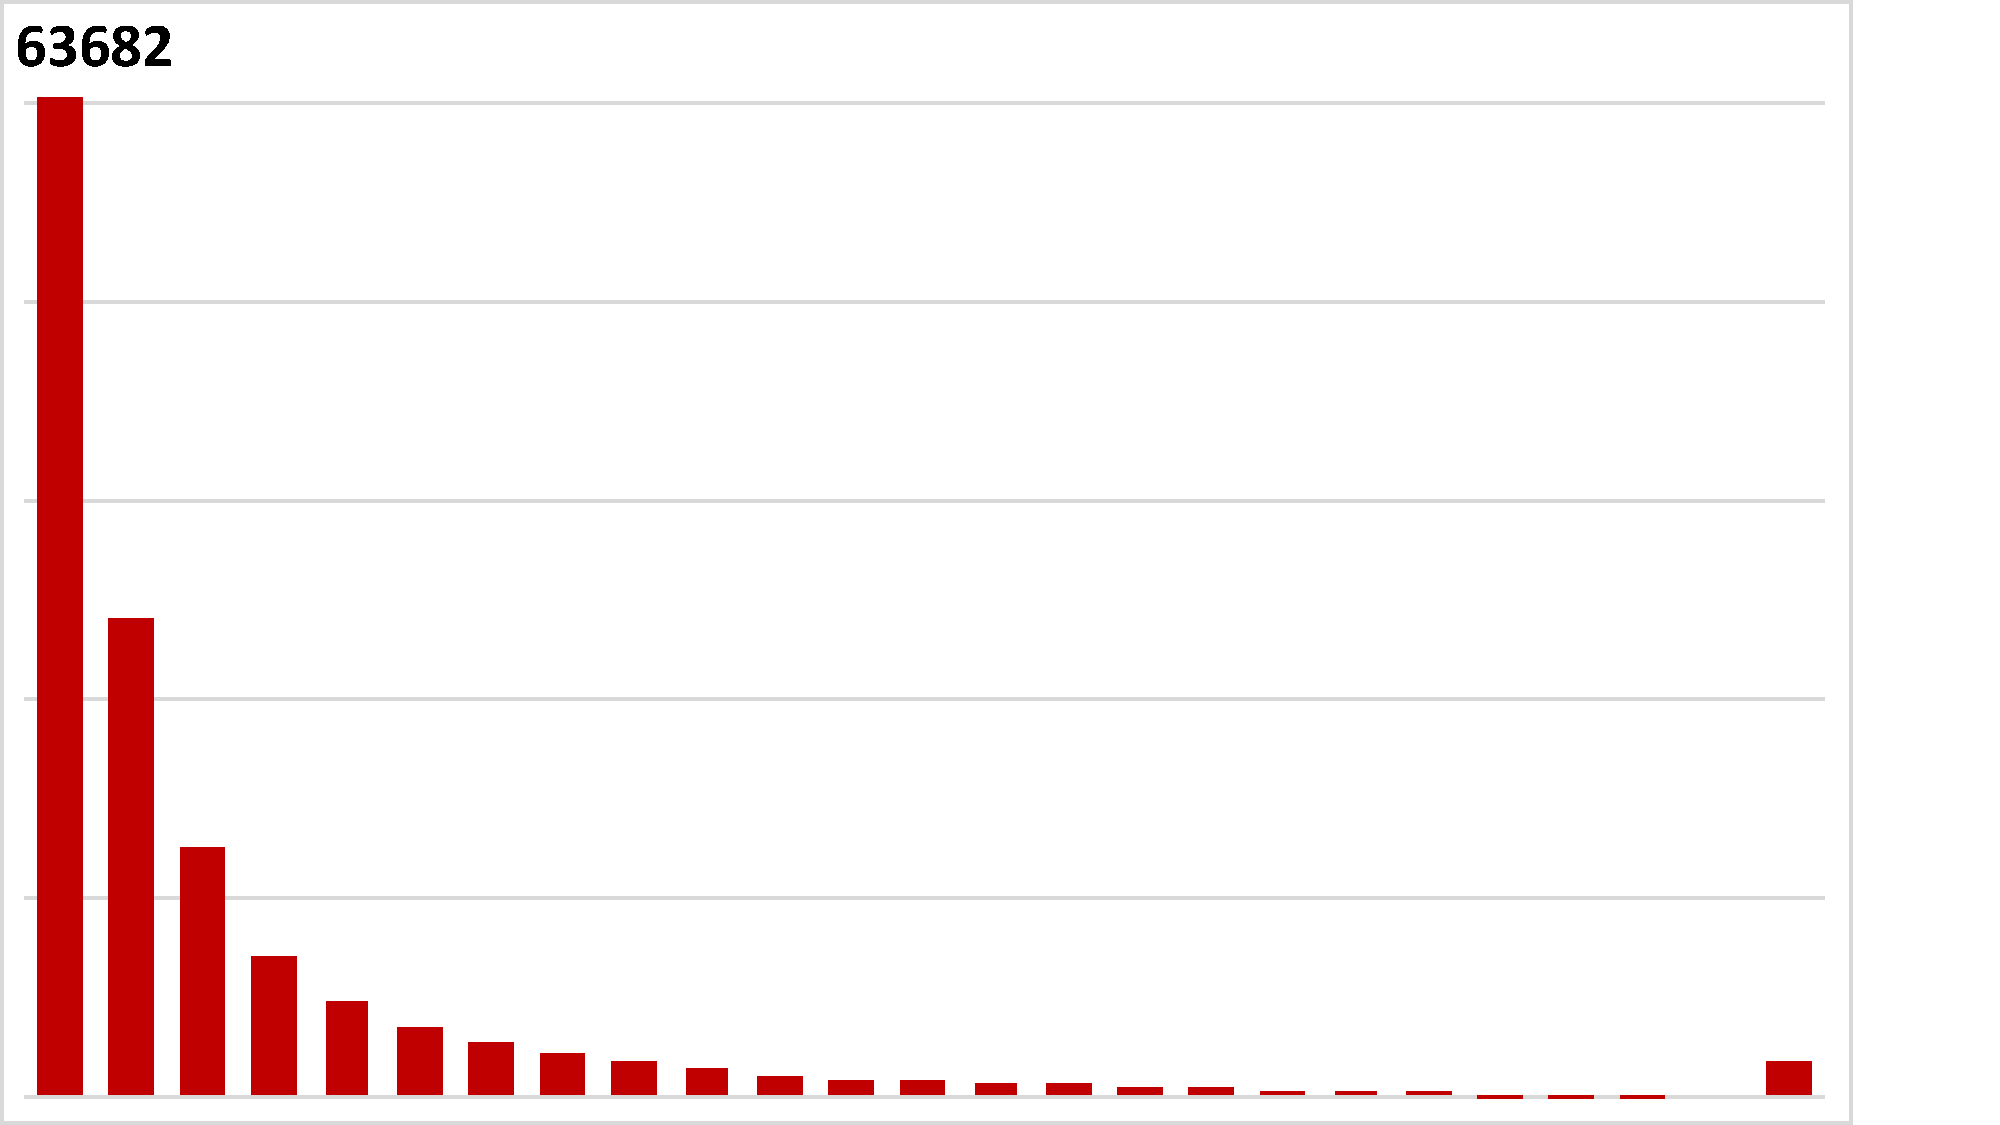
\includegraphics[width=0.9\linewidth, trim={0cm 0cm 2.5cm 0cm}, clip]{results/cloverleaf3d/lag_5/Lag5_AvgL2.pdf}
\vspace{-2mm}
\caption{Lag 40 1:27 Avg$_{L2}$ }
\end{subfigure}
\begin{subfigure}{0.195\textwidth}
\centering
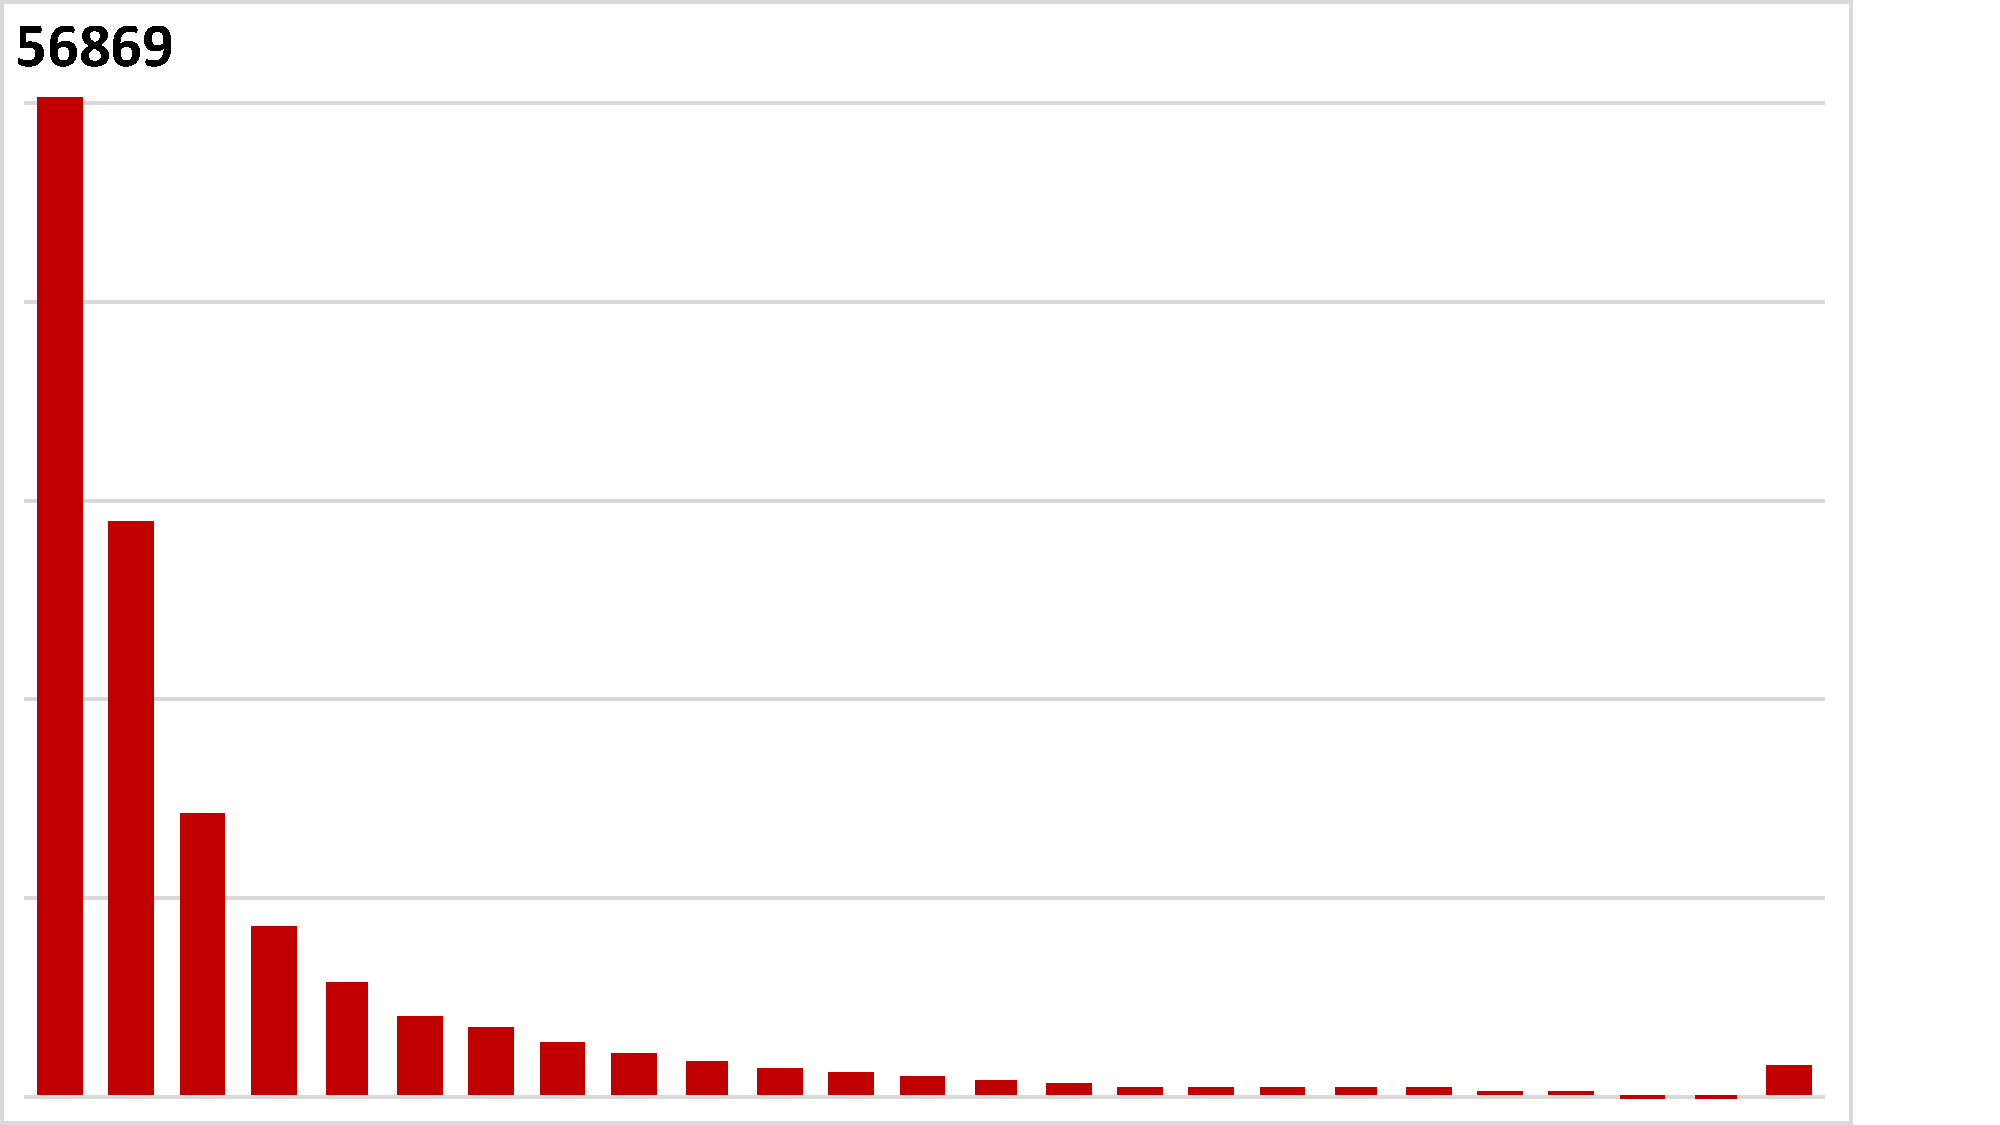
\includegraphics[width=0.9\linewidth, trim={0cm 0cm 2.5cm 0cm}, clip]{results/cloverleaf3d/lag_6/Lag6_AvgL2.pdf}
\vspace{-2mm}
\caption{Lag 40 1:64 Avg$_{L2}$ }
\end{subfigure}
\begin{subfigure}{0.195\textwidth}
\centering
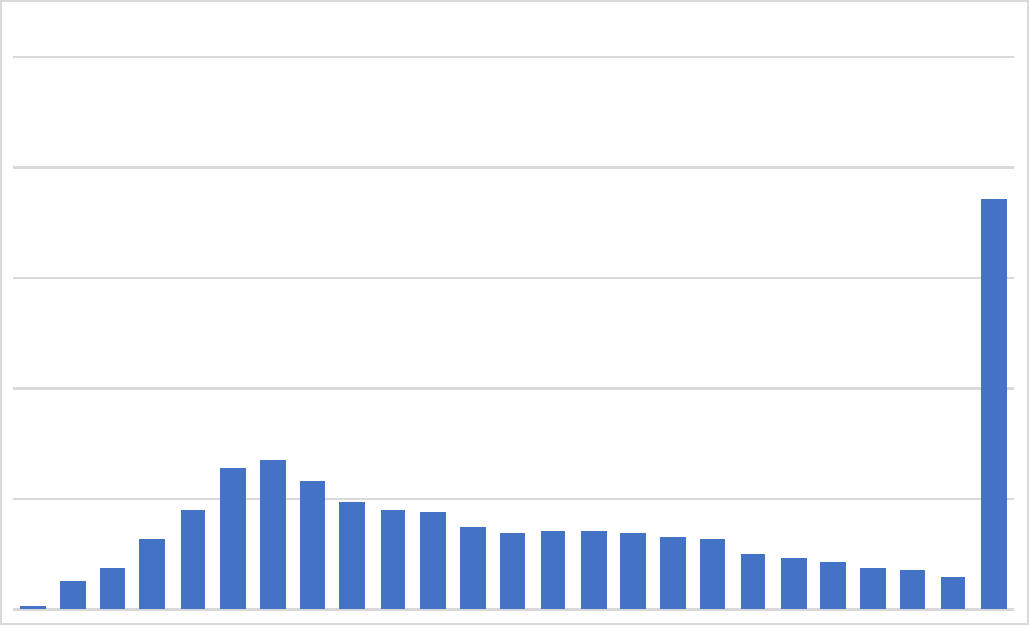
\includegraphics[width=0.9\linewidth]{results/cloverleaf3d/eul_1/Eul1_Max.pdf}
\vspace{-2mm}
\caption{Eul 20 Max$_{L2}$ }
\end{subfigure}
\begin{subfigure}{0.195\textwidth}
\centering
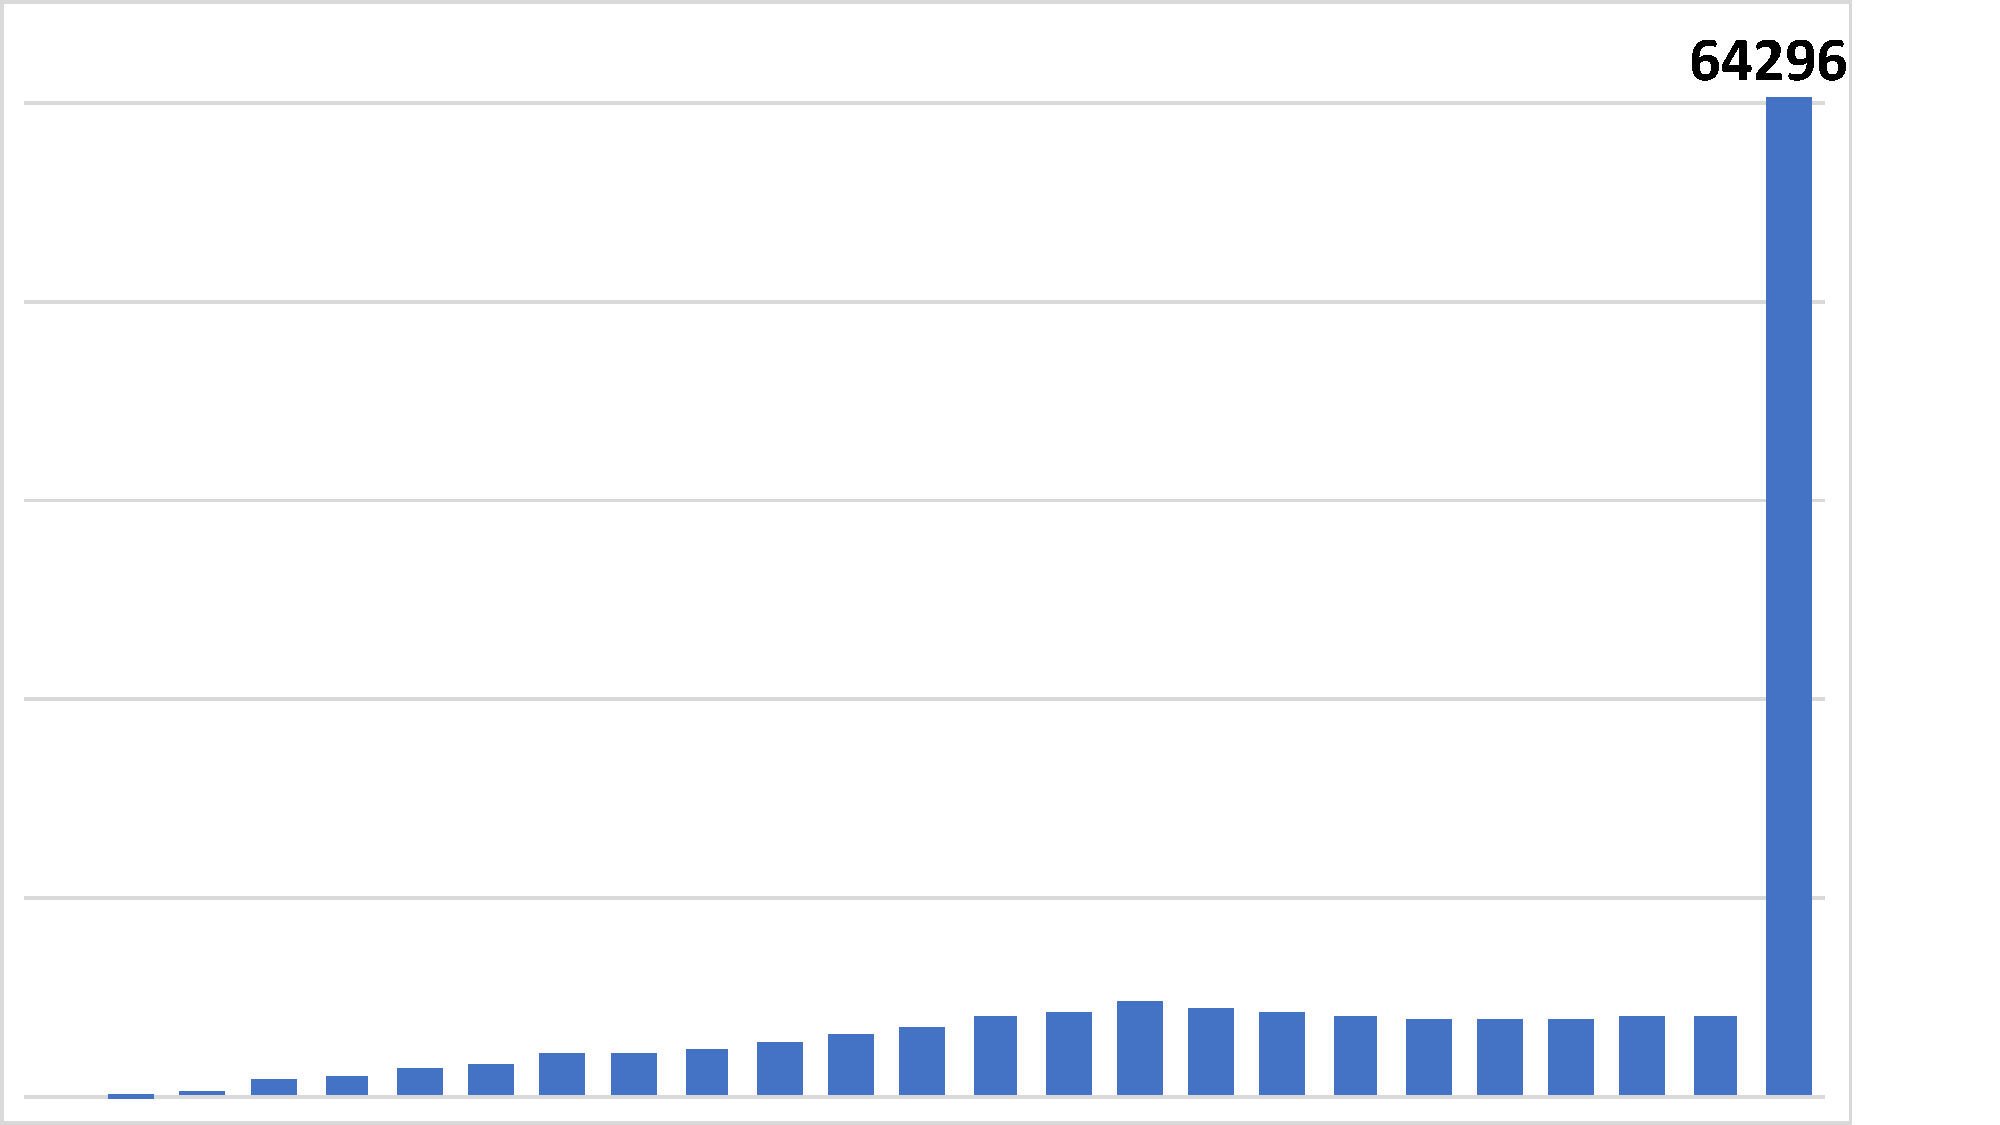
\includegraphics[width=0.95\linewidth]{results/cloverleaf3d/eul_2/Eul2_Max.pdf}
\vspace{-2mm}
\caption{Eul 40 Max$_{L2}$ }
\end{subfigure}
\hspace{0.2mm}
\begin{subfigure}{0.195\textwidth}
\centering
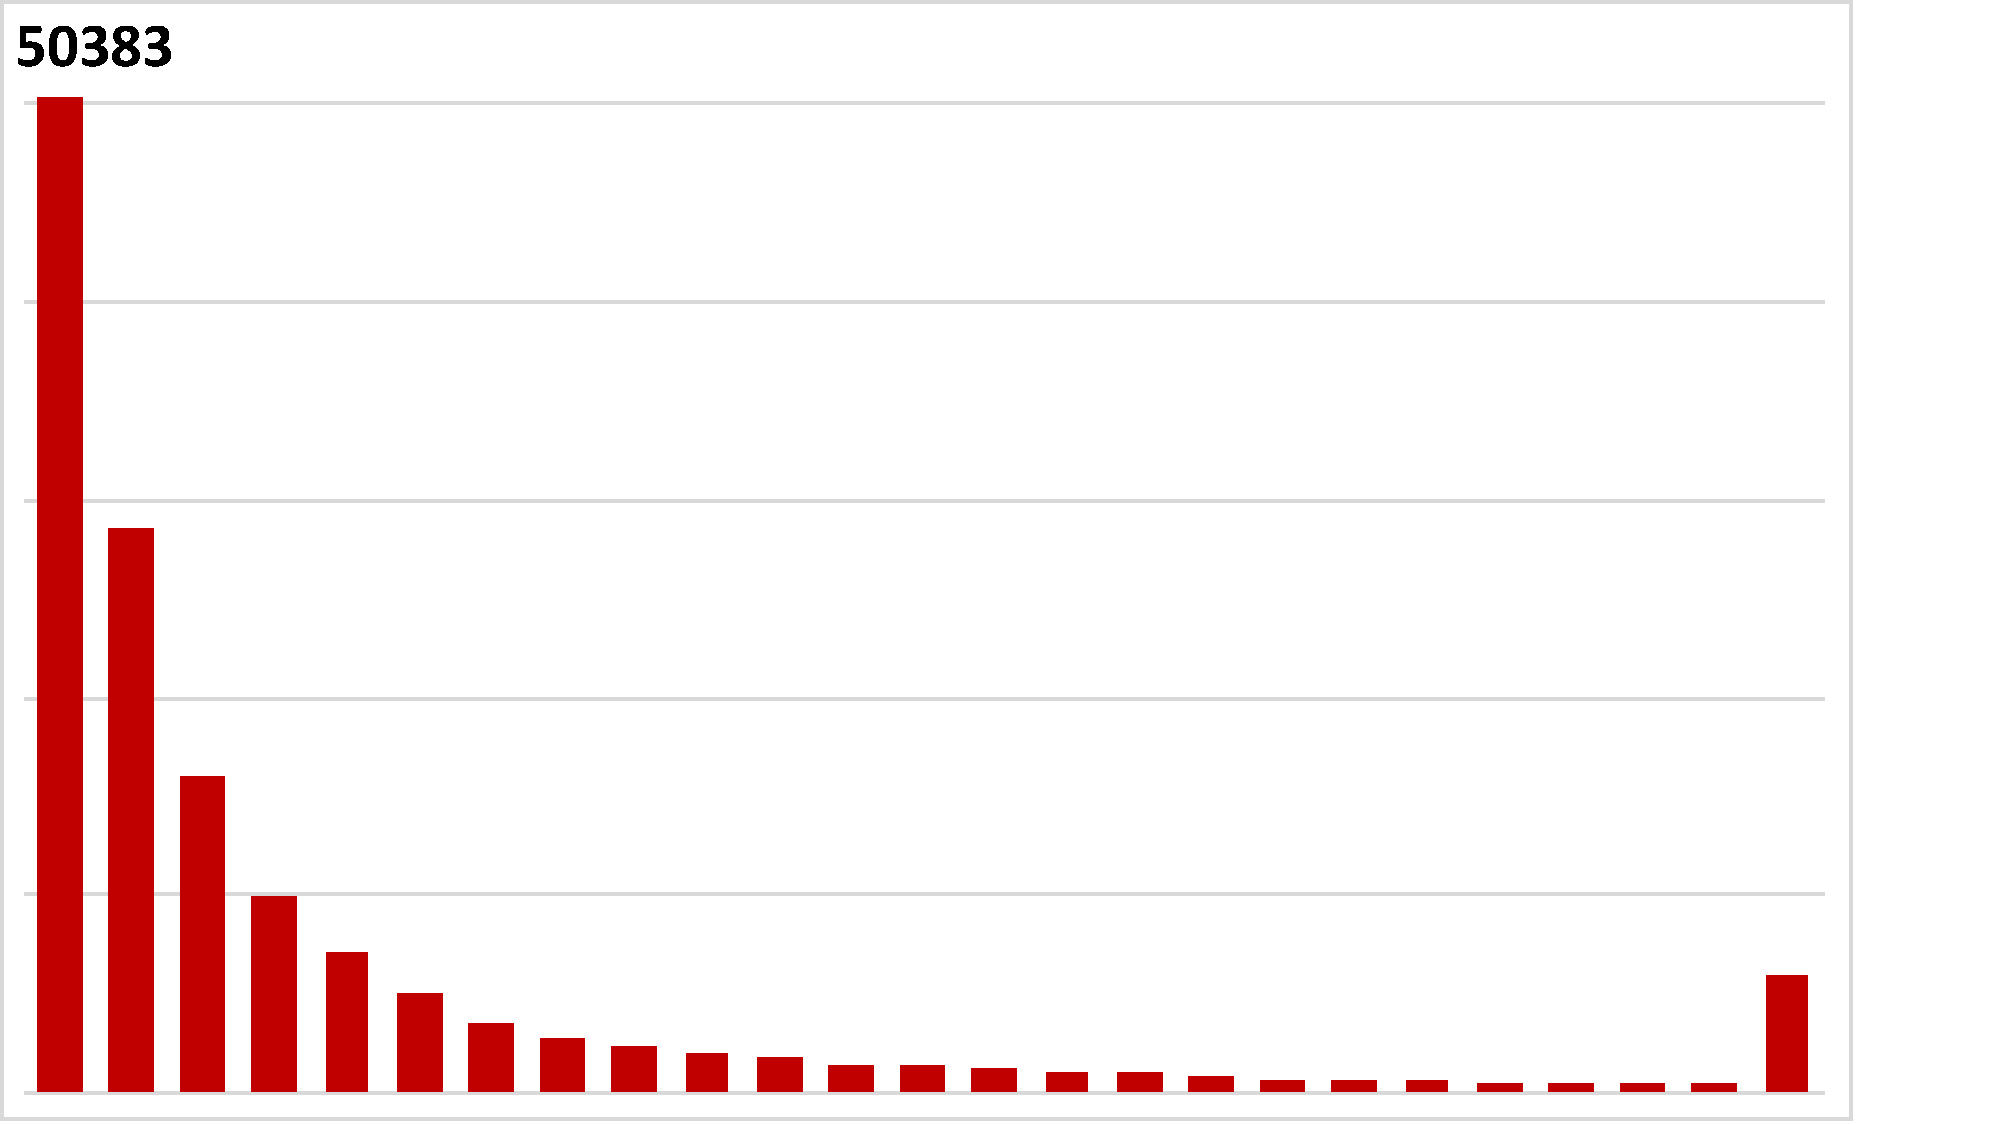
\includegraphics[width=0.9\linewidth, trim={0cm 0cm 2.5cm 0cm}, clip]{results/cloverleaf3d/lag_4/Lag4_Max.pdf}
\vspace{-2mm}
\caption{Lag 40 1:8 Max$_{L2}$ }
\end{subfigure}
\begin{subfigure}{0.195\textwidth}
\centering
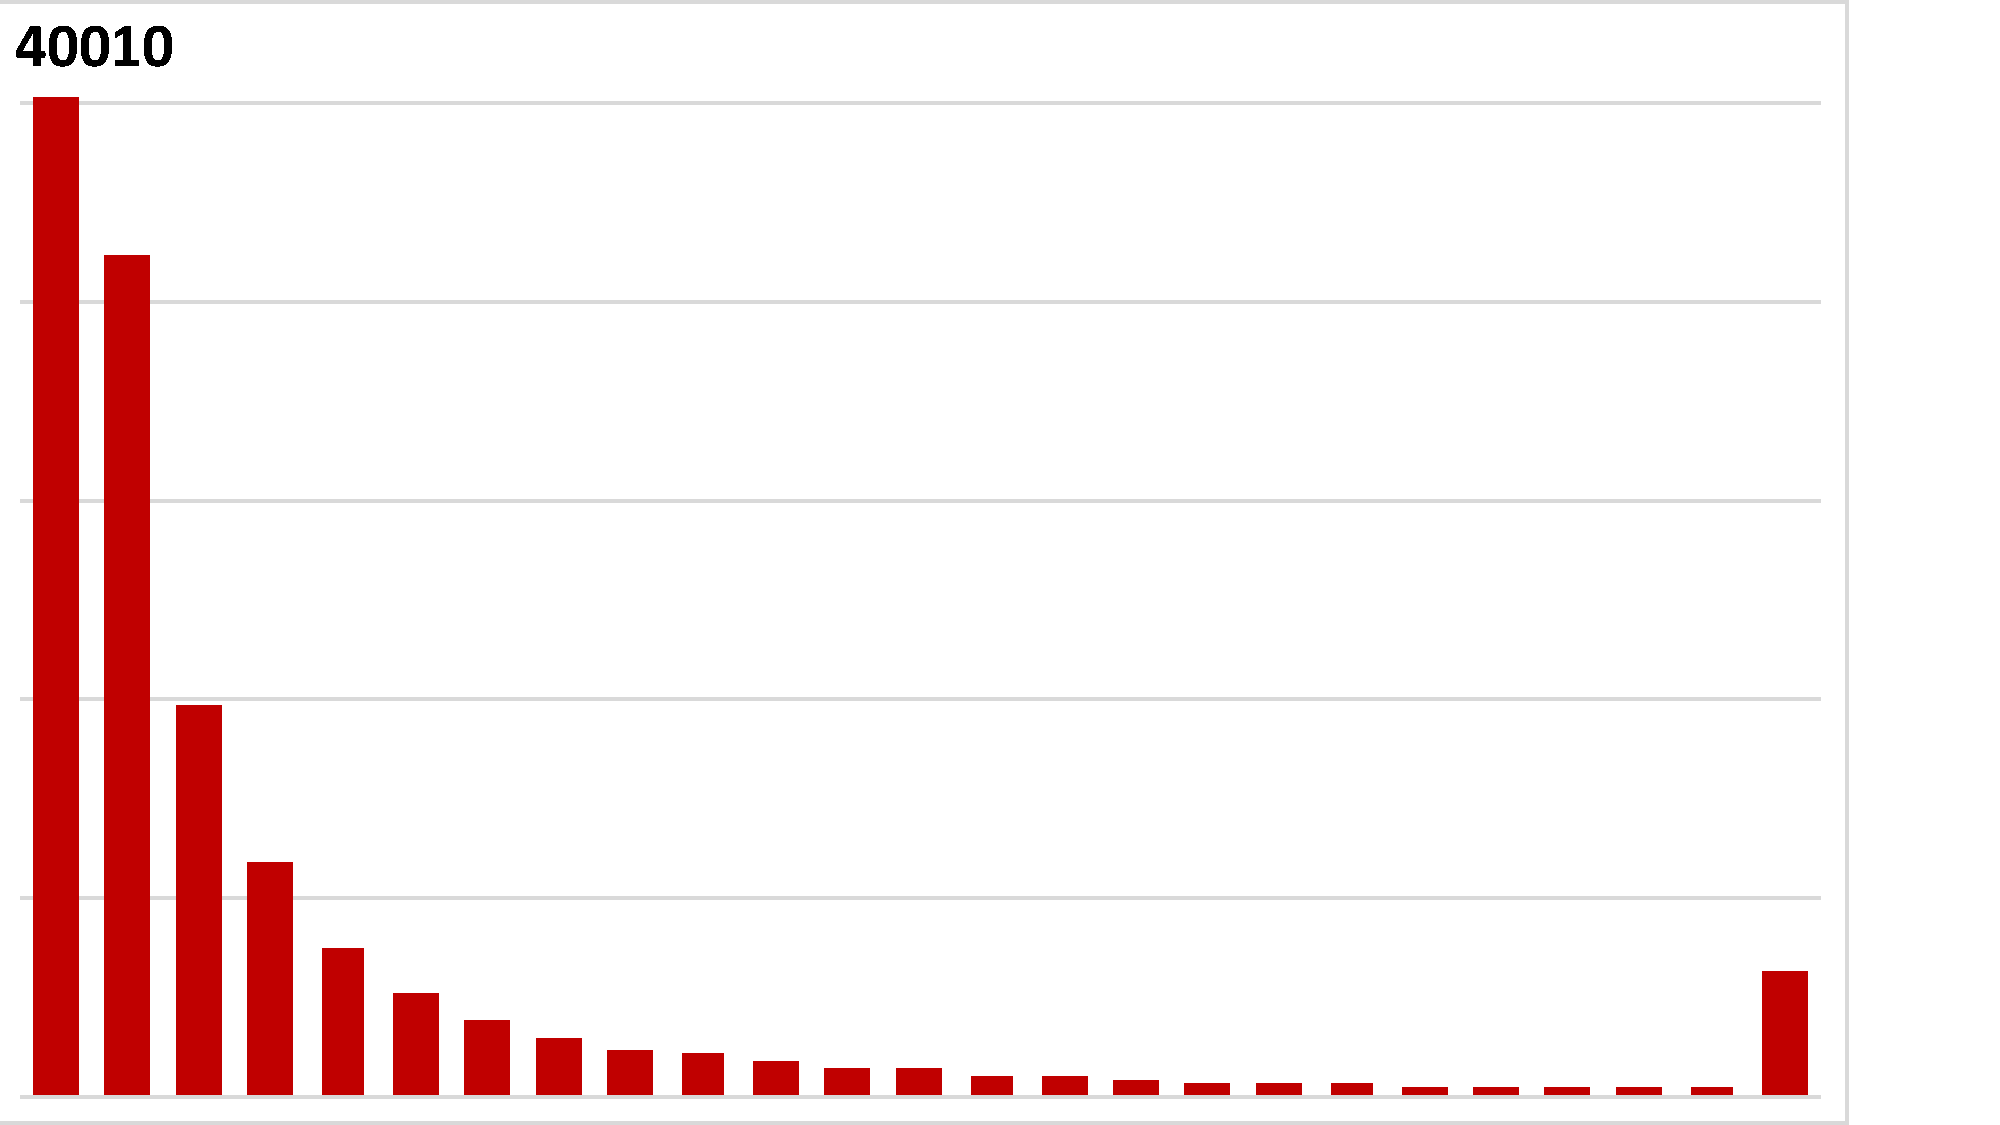
\includegraphics[width=0.9\linewidth, trim={0cm 0cm 2.5cm 0cm}, clip]{results/cloverleaf3d/lag_5/Lag5_Max.pdf}
\vspace{-2mm}
\caption{Lag 40 1:27 Max$_{L2}$}
\end{subfigure}
\begin{subfigure}{0.195\textwidth}
\centering
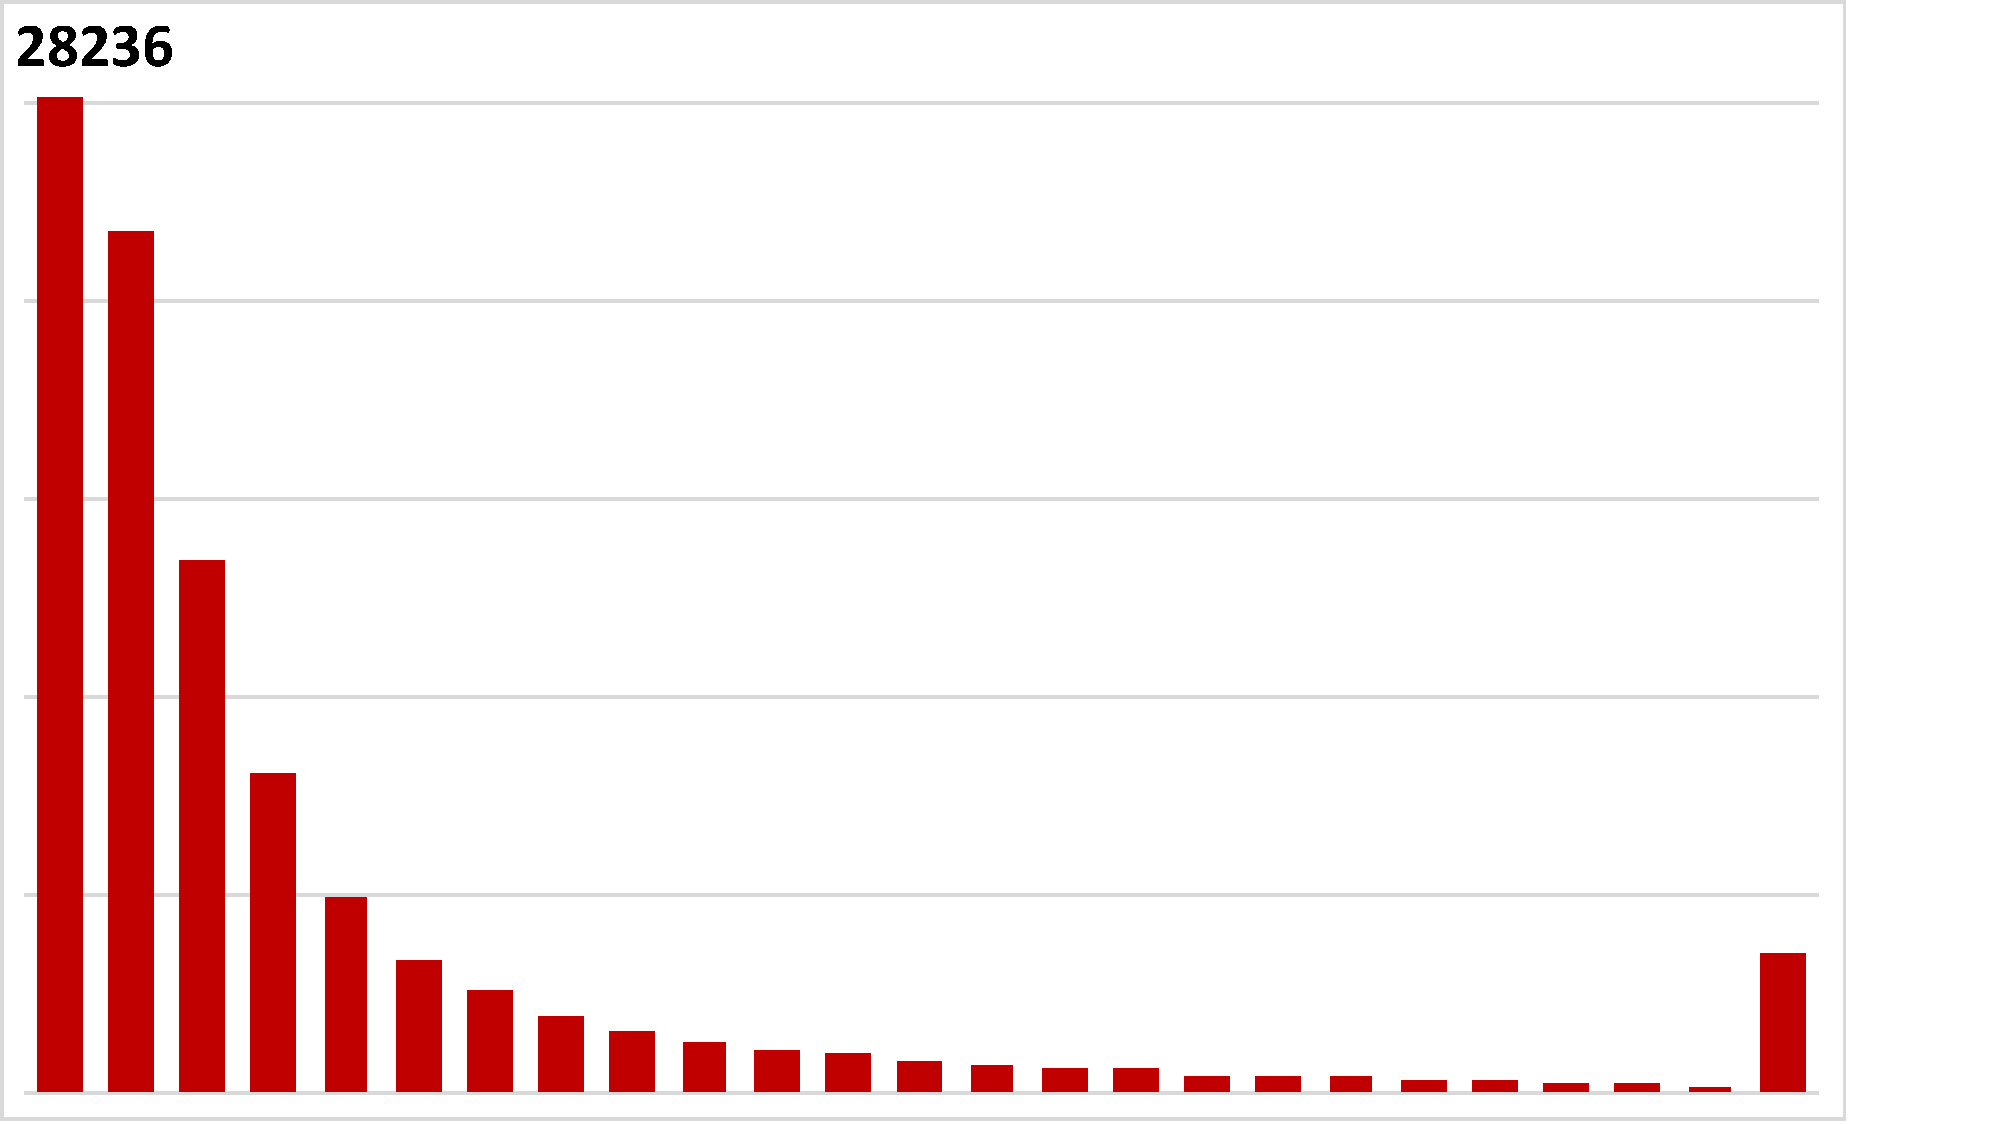
\includegraphics[width=0.9\linewidth, trim={0cm 0cm 2.5cm 0cm}, clip]{results/cloverleaf3d/lag_6/Lag6_Max.pdf}
\vspace{-2mm}
\caption{Lag 40 1:64 Max$_{L2}$}
\end{subfigure}
%\begin{subfigure}{0.24\textwidth}
%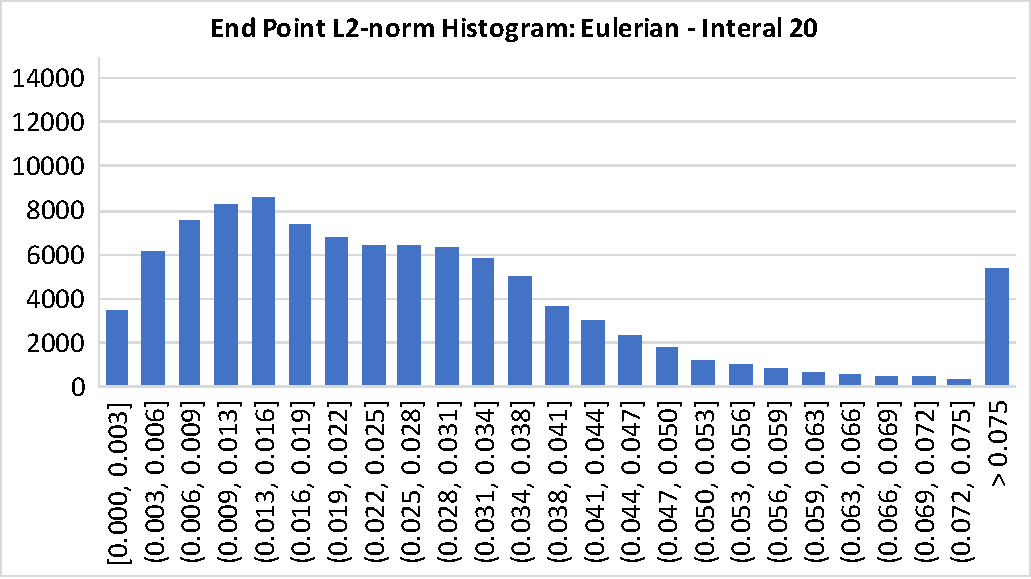
\includegraphics[width=0.9\linewidth]{results/cloverleaf3d/eul_1/Eul1_EndPt.pdf}
%\caption{Eulerian 20 End Point}
%\end{subfigure}
%\hspace{1mm}
%\begin{subfigure}{0.21\textwidth}
%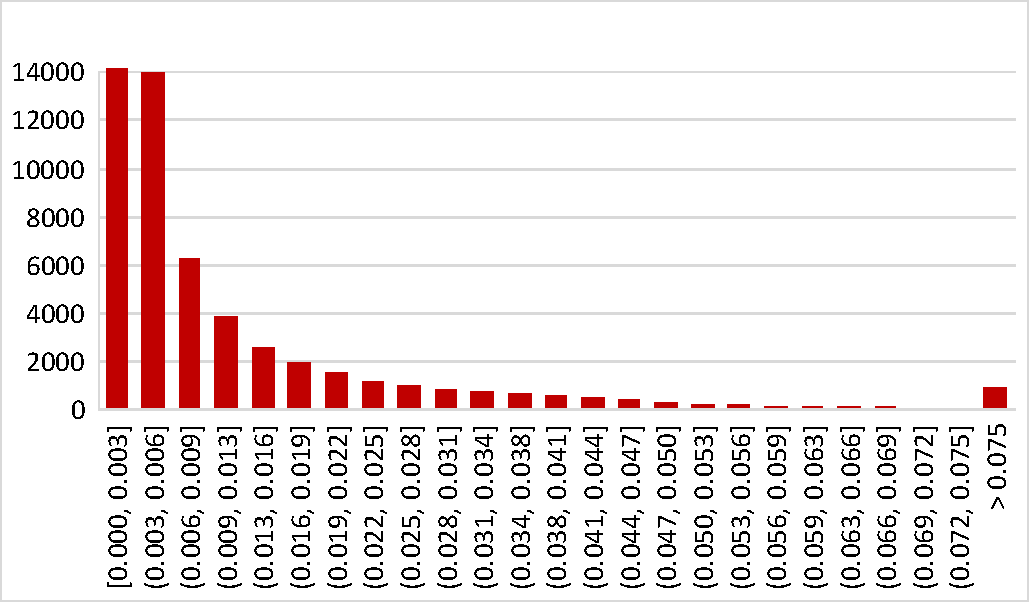
\includegraphics[width=1\linewidth]{results/cloverleaf3d/lag_4/Lag4_EndPt.pdf}
%\caption{Lagrangian 40 1:8 End Point}
%\end{subfigure}
%\hspace{1mm}
%\begin{subfigure}{0.21\textwidth}
%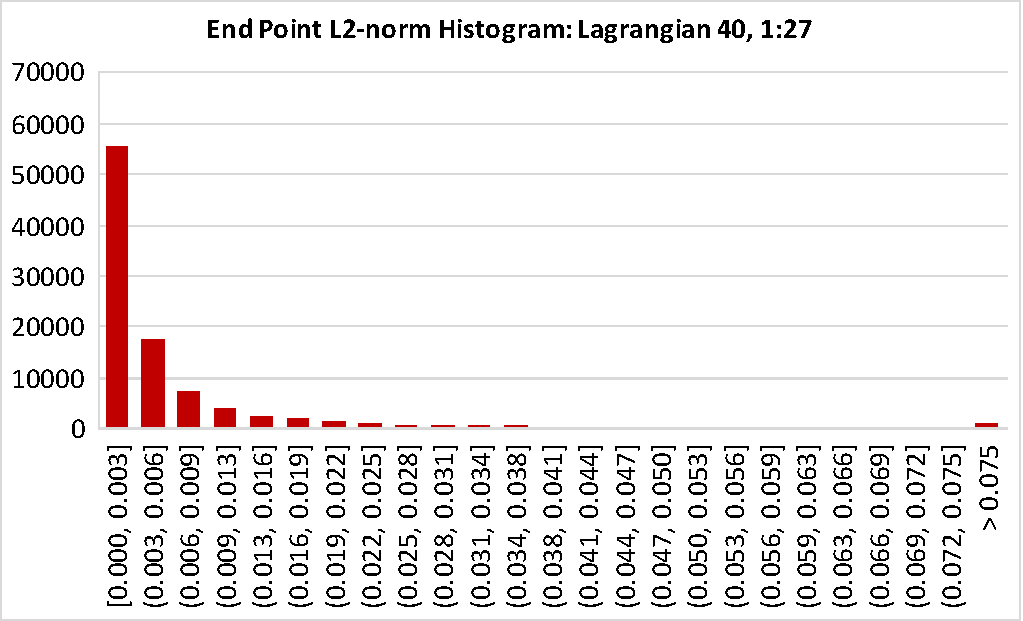
\includegraphics[width=1\linewidth]{results/cloverleaf3d/lag_5/Lag5_EndPt.pdf}
%\caption{Lagrangian 40 1:27 End Point}
%\end{subfigure}
%\hspace{1mm}
%\begin{subfigure}{0.21\textwidth}
%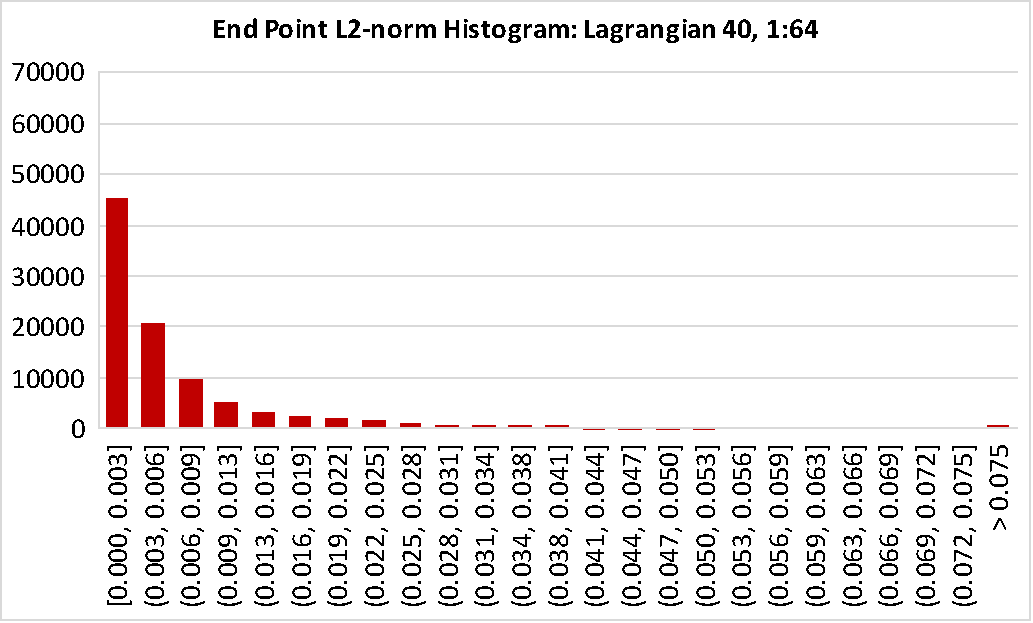
\includegraphics[width=1\linewidth]{results/cloverleaf3d/lag_6/Lag6_EndPt.pdf}
%\caption{Lagrangian 40 1:64 End Point}
%\end{subfigure}
\vspace{-3mm}
\caption{\textbf{Cloverleaf3D} experiment histograms for 100,000 test particle interpolation errors. Each plot has 25 bins, ranging from 0 to $>$0.05, with bar height encoding number of particles. Horizontal grid lines mark increments of 5,000.} 
\label{fig:clover_histograms}
\vspace{-6mm}
\end{figure*}


%\begingroup
\setlength{\tabcolsep}{-2pt}
%\renewcommand{\arraystretch}{1} % Default value: 1
\begin{table*}[!h]
%\centering
\begin{tabular}{|P{1.1cm}|P{1.1cm}|P{2.7cm}|P{1.3cm}|P{1.3cm}|P{1.5cm}|P{2cm}  N  R|P{6cm}|}
\hline
Nodes & MPI & Dimensions & Interval & Sim$_{cycle}$ & Particles & Memory & Step & DAV\% & Scatter Plots\\ 
 & Ranks & & & & /Node & /Node (MB) & & & \\ 
\hline
%\multicolumn{9}{l}{} & \\
\multicolumn{9}{l}{\textbf{          Cloverleaf3D Proxy Hydrodynamics Application }} & \multirow{13}{*}{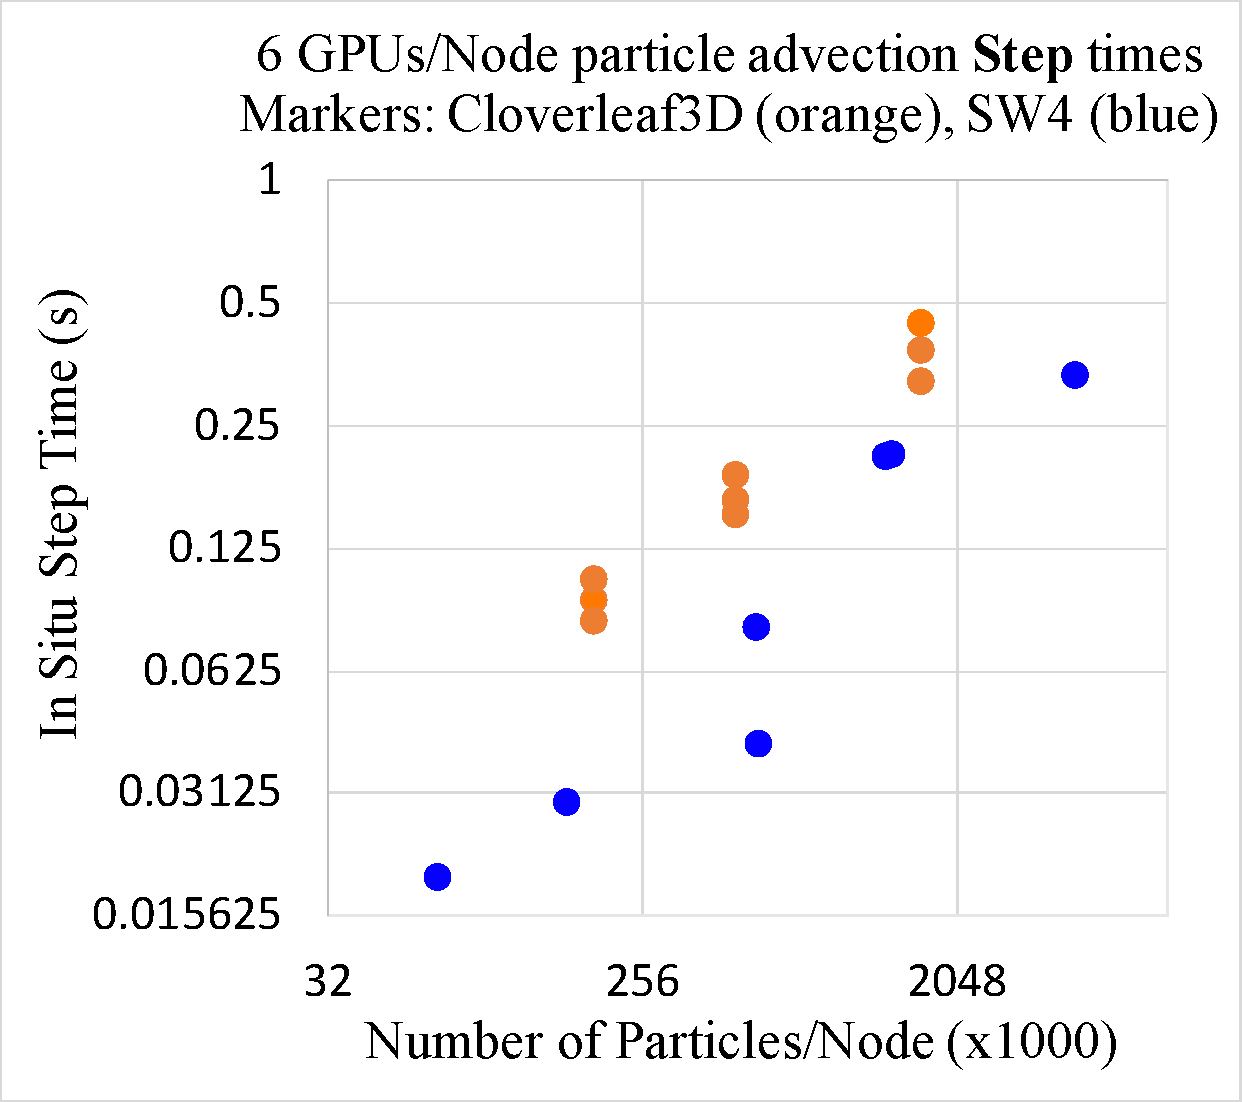
\includegraphics[width=0.93\linewidth]{images/GPU_Step.pdf}}\\
\cline{1-9}
\multirow{9}{*}{16} & \multirow{9}{*}{96} & \multirow{9}{*}{$586\times586\times586$} & 20 & 4.73 & \multirow{3}{*}{1.5M} & \multirow{3}{*}{40.2 } & 0.4475 & 9.408 & \\
\cline{4-4}
& & & 40 & 4.08 & & & 0.3221 & 7.894 & \\
\cline{4-4}
& & & 60 & 4.39 & & & 0.3838 & 8.742 & \\
\cline{4-6}%\cline{6-6}
& & & 20 & 4.50 & \multirow{3}{*}{474k} & \multirow{3}{*}{12 } & 0.1882 & 4.182 & \\
\cline{4-4}
& & & 40 & 4.14 & & & 0.1628 & 3.932 & \\
\cline{4-4}
& & & 60 & 4.33 & & & 0.1498 & 3.459 & \\
\cline{4-6}%\cline{6-6}
& & & 20 & 4.19 & \multirow{3}{*}{186k} & \multirow{3}{*}{4.2 } & 0.0925 & 2.207 & \\
\cline{4-4}
& & & 40 & 4.11 & & & 0.1043 & 2.537 & \\
\cline{4-4}
& & & 60 & 3.87 & & & 0.0830 & 2.144 & \\
\cline{1-9}
%\multicolumn{9}{l}{} & \\
\multicolumn{9}{l}{\textbf{          SW4 Seismic Modeling Simulation }} & \\
\cline{1-9}
\multirow{3}{*}{1} & \multirow{3}{*}{6} & $251\times251\times70$ & \multirow{7}{*}{200} & 0.35 & 555k & 13.89 & 0.0412 & 11.67 & \\
\cline{3-3}\cline{5-6}
& & $335\times335\times93$ & & 2.02 & 1.3M & 33.16 & 0.2125 & 10.48 & \\
\cline{3-3}\cline{5-6}  
& & $501\times501\times139$ & & 7.58 & 4.4M & 111.13 & 0.3309 & 4.365 & \multirow{13}{*}{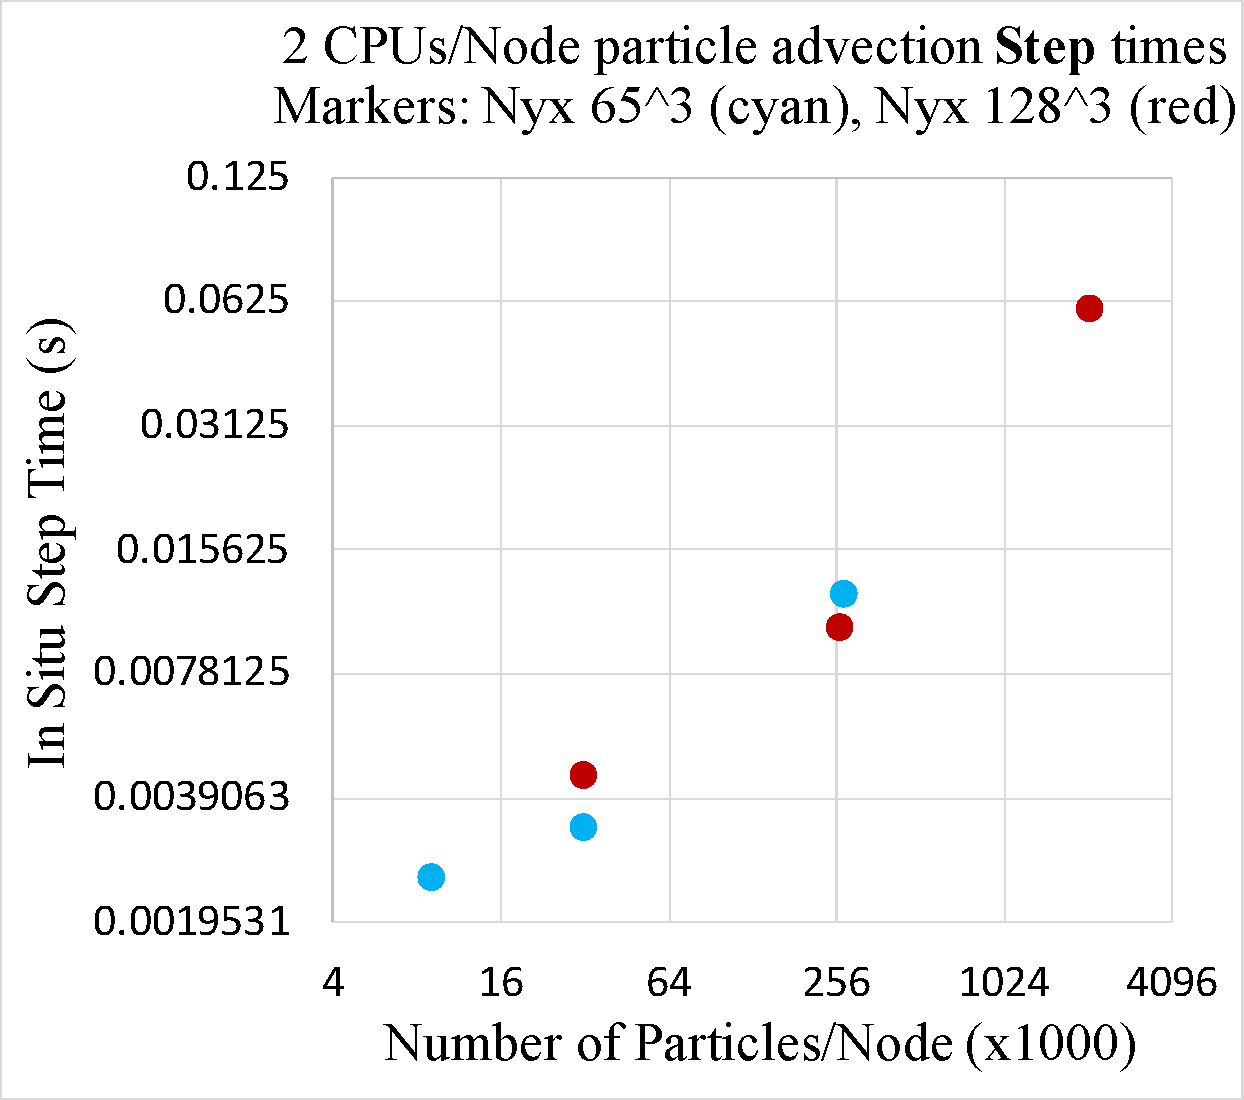
\includegraphics[width=0.93\linewidth]{images/CPU_Step.pdf}}\\
\cline{1-3}\cline{5-6}
\multirow{4}{*}{64} & \multirow{4}{*}{384} & \multirow{3}{*}{$1001\times1001\times276$} & & 1.6 & 66k & 1.6 & 0.0194 & 1.201 &  \\
\cline{6-6}
& & & & 1.5 & 146k & 3.6 & 0.0295 & 1.944 & \\
\cline{6-6}
& & & & 1.3 & 540k & 13.5 & 0.0798 & 6.175 & \\
\cline{3-3}\cline{5-6}
& & $1335\times1335\times368$ & & 2.9 & 1.2M & 31.9 & 0.2095 & 7.074 & \\
\cline{1-9}
%\multicolumn{9}{l}{} & \\
\multicolumn{9}{l}{\textbf{          Nyx Cosmology Simulation }} & \\
\cline{1-9}
\multirow{6}{*}{1} & \multirow{6}{*}{1} & \multirow{3}{*}{$65\times65\times65$} & \multirow{6}{*}{100} & \multirow{3}{*}{10.9} & 274k & 6.8 & 0.0122 & 0.112 & \\
\cline{6-6}
& & & & & 32k & 0.8 & 0.0033 & 0.030 & \\
\cline{6-6}
& & & & & 9k & 0.2 & 0.0025 & 0.023 & \\
\cline{3-3}\cline{5-6}
& & \multirow{3}{*}{$129\times129\times129$} & & \multirow{3}{*}{88.3} & 2.1M & 53.6 & 0.0596 & 0.067 & \\
\cline{6-6}
& & & & & 262k & 6.5 & 0.0101 & 0.011 & \\
\cline{6-6}
& & & & & 32k & 0.8 & 0.0044 & 0.005 & \\
\hline
\end{tabular}
\vspace{-3mm}
\caption{\textit{In situ} encumbrance evaluation and experiment configurations for our three simulation codes.}
\label{table:encumbrance}
\vspace{-5mm}
\end{table*}
\endgroup

Table~\ref{table:encumbrance} contains the results of our experiments for this campaign using all three simulation codes.
%
In this discussion, we assume a simulation can afford to spend 10\% to 20\% on \textit{in situ} processing routines and refer to this as the \textbf{budget}. 
%
Although this might not hold true for every simulation, this estimate is based on interactions with computational scientists and thus, we believe this is a reasonable working estimate.
%
The \textbf{Step} and \textbf{DAV\%} columns in Table~\ref{table:encumbrance} redundantly encode the value in each cell using cell background color (white to pure red hue for the ranges [0,0.75]~(\textbf{Step} in seconds) and [0,20]~(\textbf{DAV\%}), respectively).
%

For \textbf{ISR-2}, i.e., memory costs, we observe that across all experiments, the largest usage of runtime memory was approximately 112 MB.
%
Each Summit node has multiple GBs of memory on CPU~(512) and GPU~(16), and we believe extracting a Lagrangian representation increases the cost of memory on the simulation by approximately one simulation ``field''.
%
We note that simulations can have tens to hundreds of fields defined on the simulation grid and thus, this cost would likely be considered acceptable for most simulations.
%
Our reporting of memory usage is contained in Table~\ref{table:encumbrance}.

\subsubsection{Cloverleaf3D Hydrodynamics Proxy Simulation}
For the Cloverleaf3D simulation, we considered 3 options for number of particles and interval, and 1 option for grid size and concurrency.
%
In particular, we are interested in the \textit{in situ} encumbrance (\textbf{ISR-1}) of varying particle advection workloads, i.e., the number of particles. 
%
We note that each node used 6 GPUs for particle advection and that they all access the same shared memory.
%
For our specific grid size and domain decomposition, each MPI rank operated on over 2M grid points and the Sim$_{cycle}$ was usually between 4-5 seconds. 
%
Overall, we observe an increase in \textbf{Step} costs as the number of particles advected per node increases.
%
Given, the Sim$_{cycle}$ remained relatively stable, the increase in \textbf{Step} is clearly matched by the \textbf{DAV\%} trend.
%

For this integration, we observed that as the number of particles increases from 186k to 474k (2.5X increase) that the cost of performing particle advection only increases by approximately 1.6X. 
%
For the next workload increase, i.e., sampling 1.5M particles ($\sim$3X increase), the cost of performing particle advection increases by approximately 2X.
%
By running the same workload multiple times, we capture variation in the costs within a workload.
%
The variation in the \textbf{Step} cost is greater when the workload is larger and we attribute this to the increased memory allocation and memory transfer costs each step.
%
This is relevant particularly on GPUs where the initial setup cost can be high.
%
%An approximately 0.4\% range in DAV\% across multiple runs using the smallest workload (186k), and up to 1\% variation in DAV\% for the largest workload (1.5M). 
%

Overall, for \textbf{ISR-1}, we found that for our set of experiments increasing the number of particles by 8X results in the \textit{in situ} encumbrance increasing by 3X-4X with the Sim$_{cycle}$ relatively stable.
%
The cost of a single \textbf{Step} to calculate the Lagrangian representation for Cloverleaf3D was as low as 0.08 seconds and in all cases, below half a second, thus, remaining within our identified \textbf{budget}.

\subsubsection{SW4 Seismic Wave Propagation Simulation}
For the SW4 simulation, we considered 2 concurrencies: 1 compute node (6 MPI ranks, GPUs) and 64 compute nodes (384 MPI ranks, GPUs).
%

In the first case, i.e., using 1 compute node and 6 MPI ranks, we considered three grid sizes, each using a proportional number of particles (1:8).
%
We increase the number of particles proportionately, rather than holding it constant, since we believe this would be a more representative of a workload.
%
These results in our empirical study highlight the impact of an increasing grid size on \textbf{ISR-1} and the relation to Sim$_{cycle}$.
%
For the smallest grid size, 555k particles per node are advected every cycle.
%
Although the cost of a particle advection \textbf{Step} is low (0.041s), the \textbf{DAV\%} is over 10\% because the Sim$_{cycle}$ is very small (0.035s) in this case.
%
In contrast, for the largest grid size (each rank operated on 5.8M grid points), we advected 4.4M particles per node and observed a proportional increase in \textbf{Step} cost, but half as much time was spent by the simulation on \textbf{DAV\%}.
%
This is due to the higher Sim$_{cycle}$ for the larger grid size.
%
We note this trend would be expected for computational simulations as they increase in resolution per compute node.
%
%Simulations can require anything between a few seconds to several minutes to complete a cycle.

In the second case, i.e., using 64 compute nodes and 384 MPI ranks, we ran SW4 four times. 
%
Three times with one grid size to observe \textit{in situ} encumbrance for varying particle advection workloads, and one time using a larger grid with 1:8 particles per node.
%
Similar to the Cloverleaf3D experiments, we observed a steady increase in \textbf{Step} and \textbf{DAV\%} as the number of particles per node increases.
%
For the fixed grid size, an 8X increase in the particle advection workload results in an approximately 4X increase, considering Sim$_{cycle}$ with small variability.
%
However, as we increased the grid size, and consequentially, the workload from 540k to 1.2M particles per node ($\sim$2X), although the \textbf{Step} cost increased by over 2.6X, \textbf{DAV\%} increased by less than 1\%.
%

Overall, we first observed that the \textbf{DAV\%} is closely related to the Sim$_{cycle}$. 
%
Although extracting a Lagrangian representation might place a higher encumbrance on a simulation with a small Sim$_{cycle}$ value, for all grid sizes considered the \textit{in situ} encumbrance, i.e., \textbf{DAV\%}, of the corresponding workload remained within our expected \textbf{budget} and the cost of \textbf{Step} was less than half a second in each case.

\subsubsection{Nyx Cosmology Simulation}
Unlike our previous experiments, the Nyx simulation and Lagrangian filter use OpenMP for parallelism, i.e., particle advection is performed using all the CPU cores on a compute node.
%
We considered 3 options for number of particles and 2 options for grid size.
%

First, focusing on the impact of an increase in the grid size on \textbf{ISR-1}, we found a small increase ($<$1.5X) in the absolute cost of a particle advection \textbf{Step} for the same workload, albeit interpolating a grid 8X in size.
%
Further, in the context of \textbf{DAV\%}, the Sim$_{cycle}$ cost increases proportionately to the increase in grid size (8X).
%
Thus, the \textbf{DAV\%} reduces as the simulation grid size increases.
%
Next, for \textbf{ISR-1} across workloads using a fixed grid size, for the smaller grid we observed less than a 5X increase when going from 9k particles to 274k particles per node (30X increase in workload).
%
For the larger grid, a 65X increase in workload resulted in a 13X increase in \textbf{Step} time.

The most interesting finding of these experiments was that using the CPUs, a single particle advection step for the number of particles we considered, costs less than 6 GPUs.
%
For example, the \textbf{Step} cost for 2.1M particles on 2 CPUs is less than half compared to the \textbf{Step} cost for 1.3M and 1.5M particles using 6 GPUs.
%
We do note there are differences, such as 6 GPUs (i.e., 6 MPI ranks) accessing the same memory versus 1 MPI rank on 2 CPUs accessing memory.
%
Although this outcome is likely not surprising (given our knowledge of memory allocation and transfer times for GPUs versus CPUs), this finding certainly encourages future research on how to utilize compute resources if the \textit{in situ} routine frequency is very high (every cycle in our study).
%

Overall, considering the larger Sim$_{cycle}$ times and low memory latency when parallelizing using CPUs, the highest \textit{in situ} encumbrance we observed to extract a Lagrangian representation was 0.1\% of the simulation time.

%\begin{figure*}
\begin{subfigure}{0.195\textwidth}
\centering
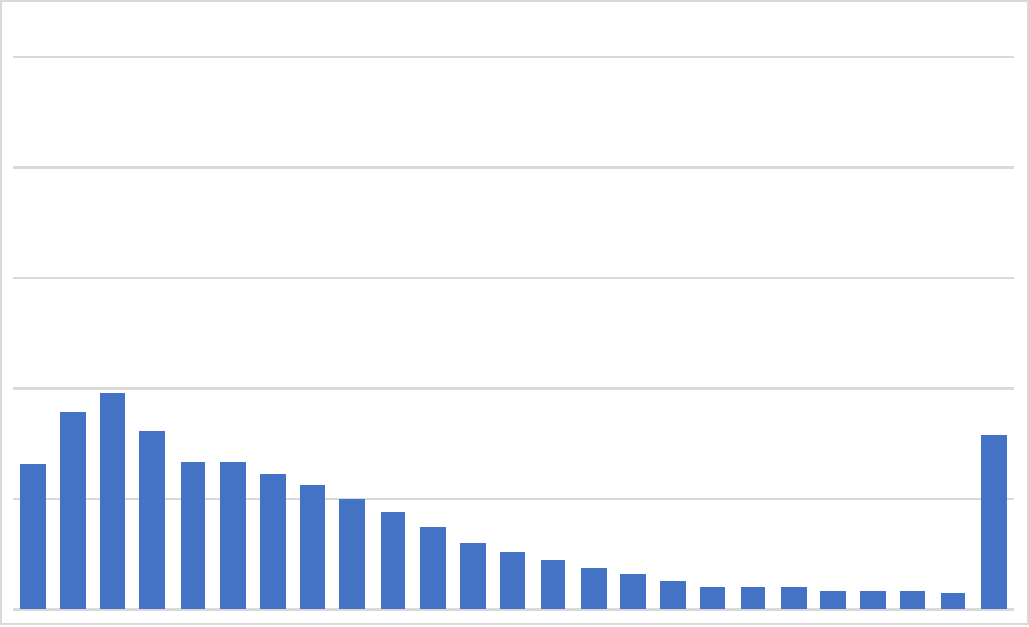
\includegraphics[width=0.9\linewidth]{results/cloverleaf3d/eul_1/Eul1_AvgL2.pdf}
\vspace{-2mm}
\caption{Eul 20 Avg$_{L2}$ L2 }
\end{subfigure}
\begin{subfigure}{0.195\textwidth}
\centering
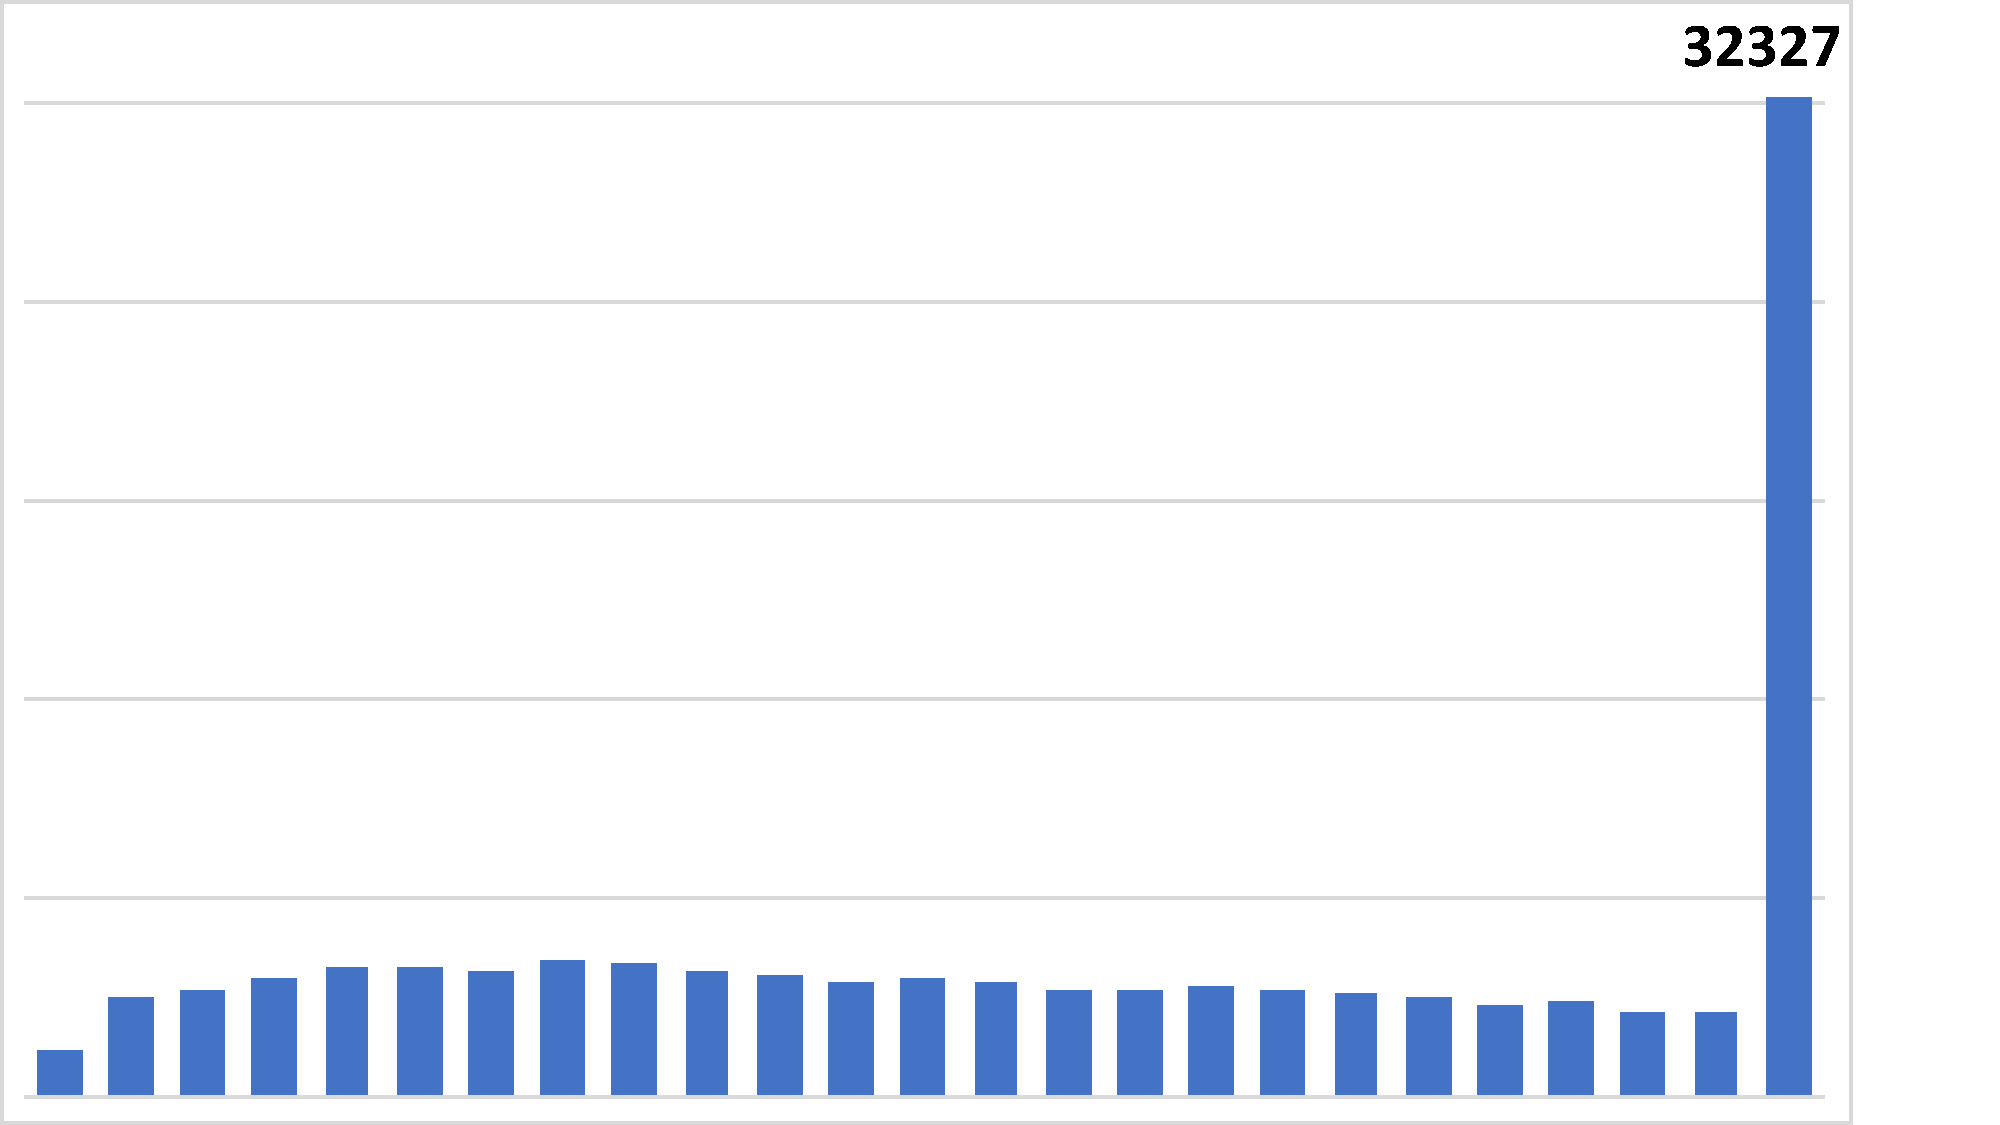
\includegraphics[width=0.95\linewidth]{results/cloverleaf3d/eul_2/Eul2_AvgL2.pdf}
\vspace{-2mm}
\caption{Eul 40 Avg$_{L2}$ L2 }
\end{subfigure}
\begin{subfigure}{0.195\textwidth}
\centering
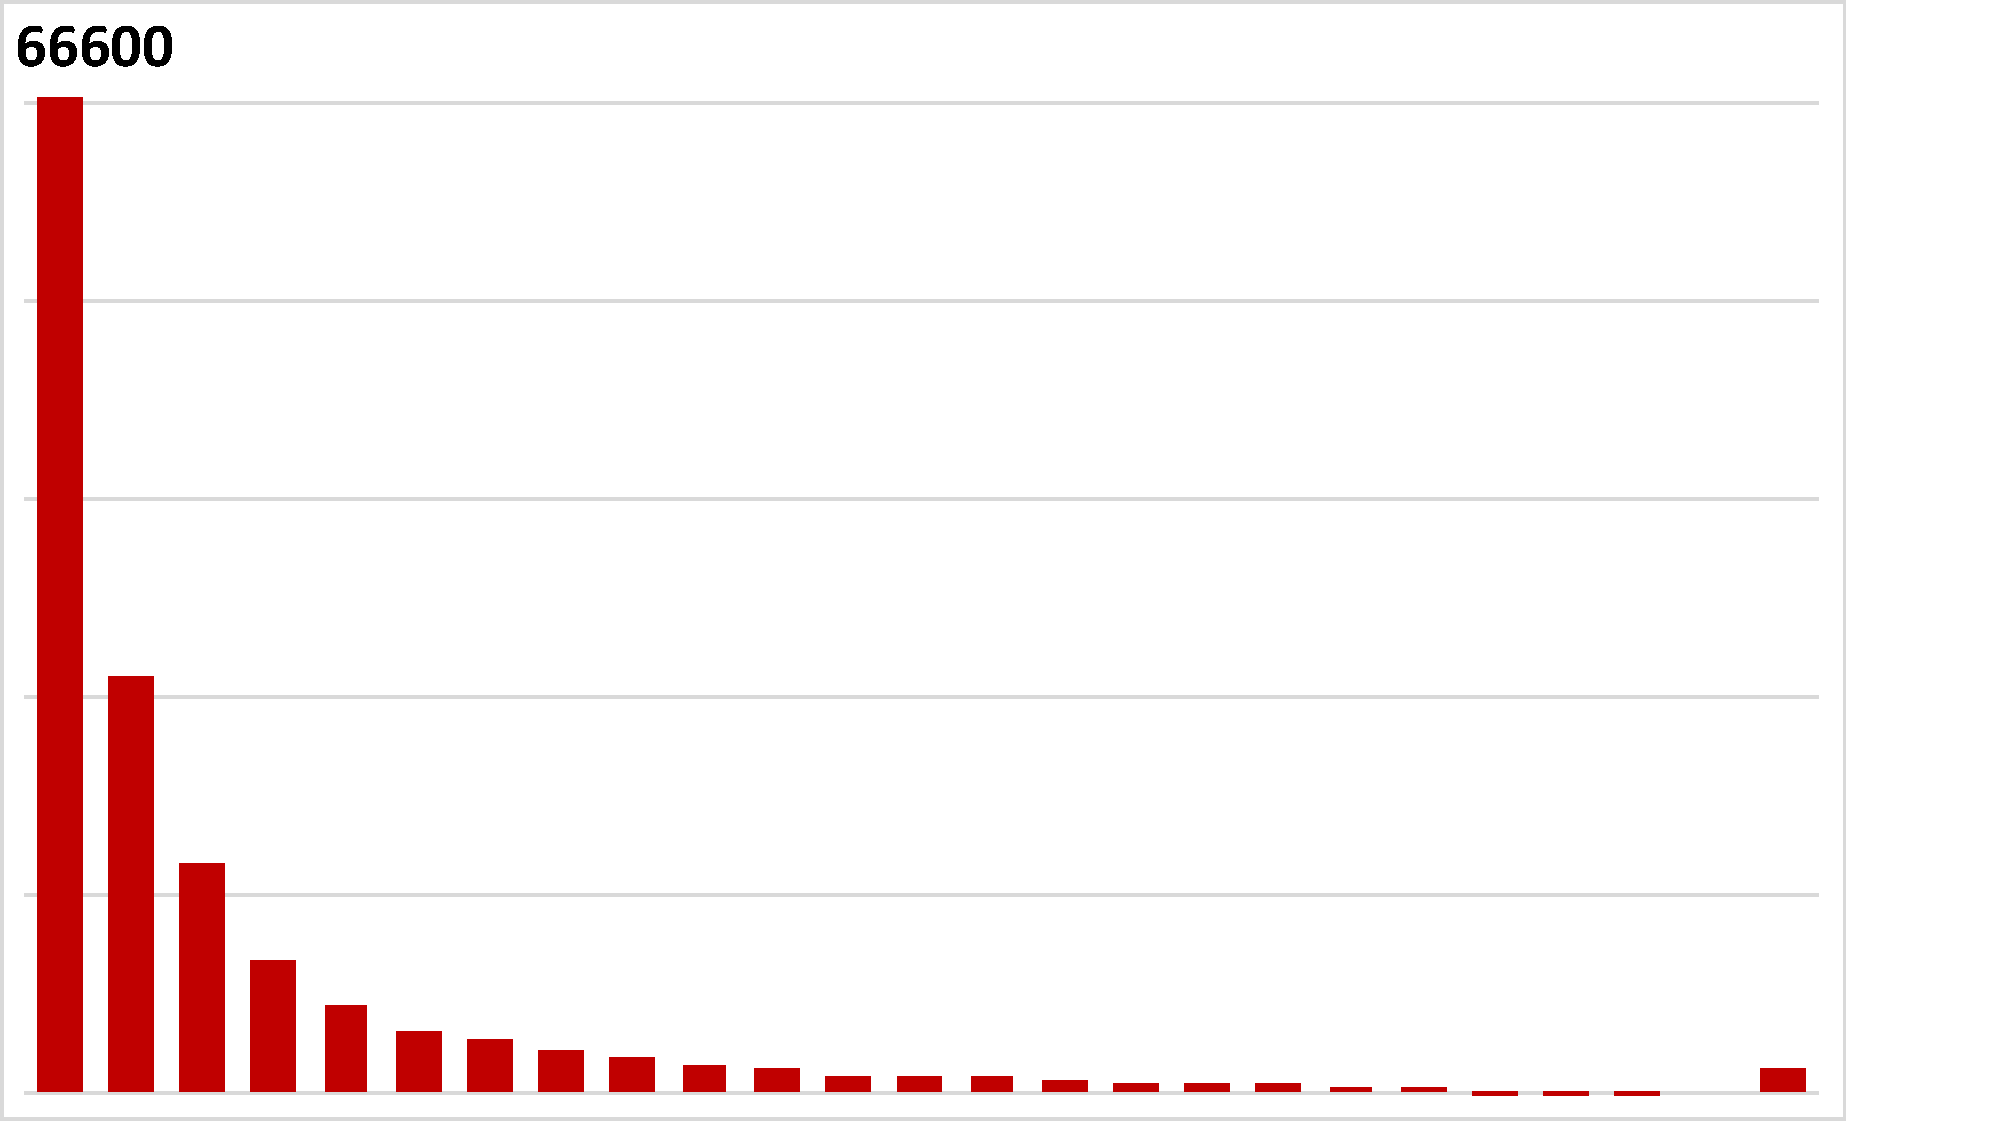
\includegraphics[width=0.9\linewidth, trim={0cm 0cm 2.5cm 0cm}, clip]{results/cloverleaf3d/lag_4/Lag4_AvgL2.pdf}
\vspace{-2mm}
\caption{Lag 40 1:8 Avg$_{L2}$ }
\end{subfigure}
\begin{subfigure}{0.195\textwidth}
\centering
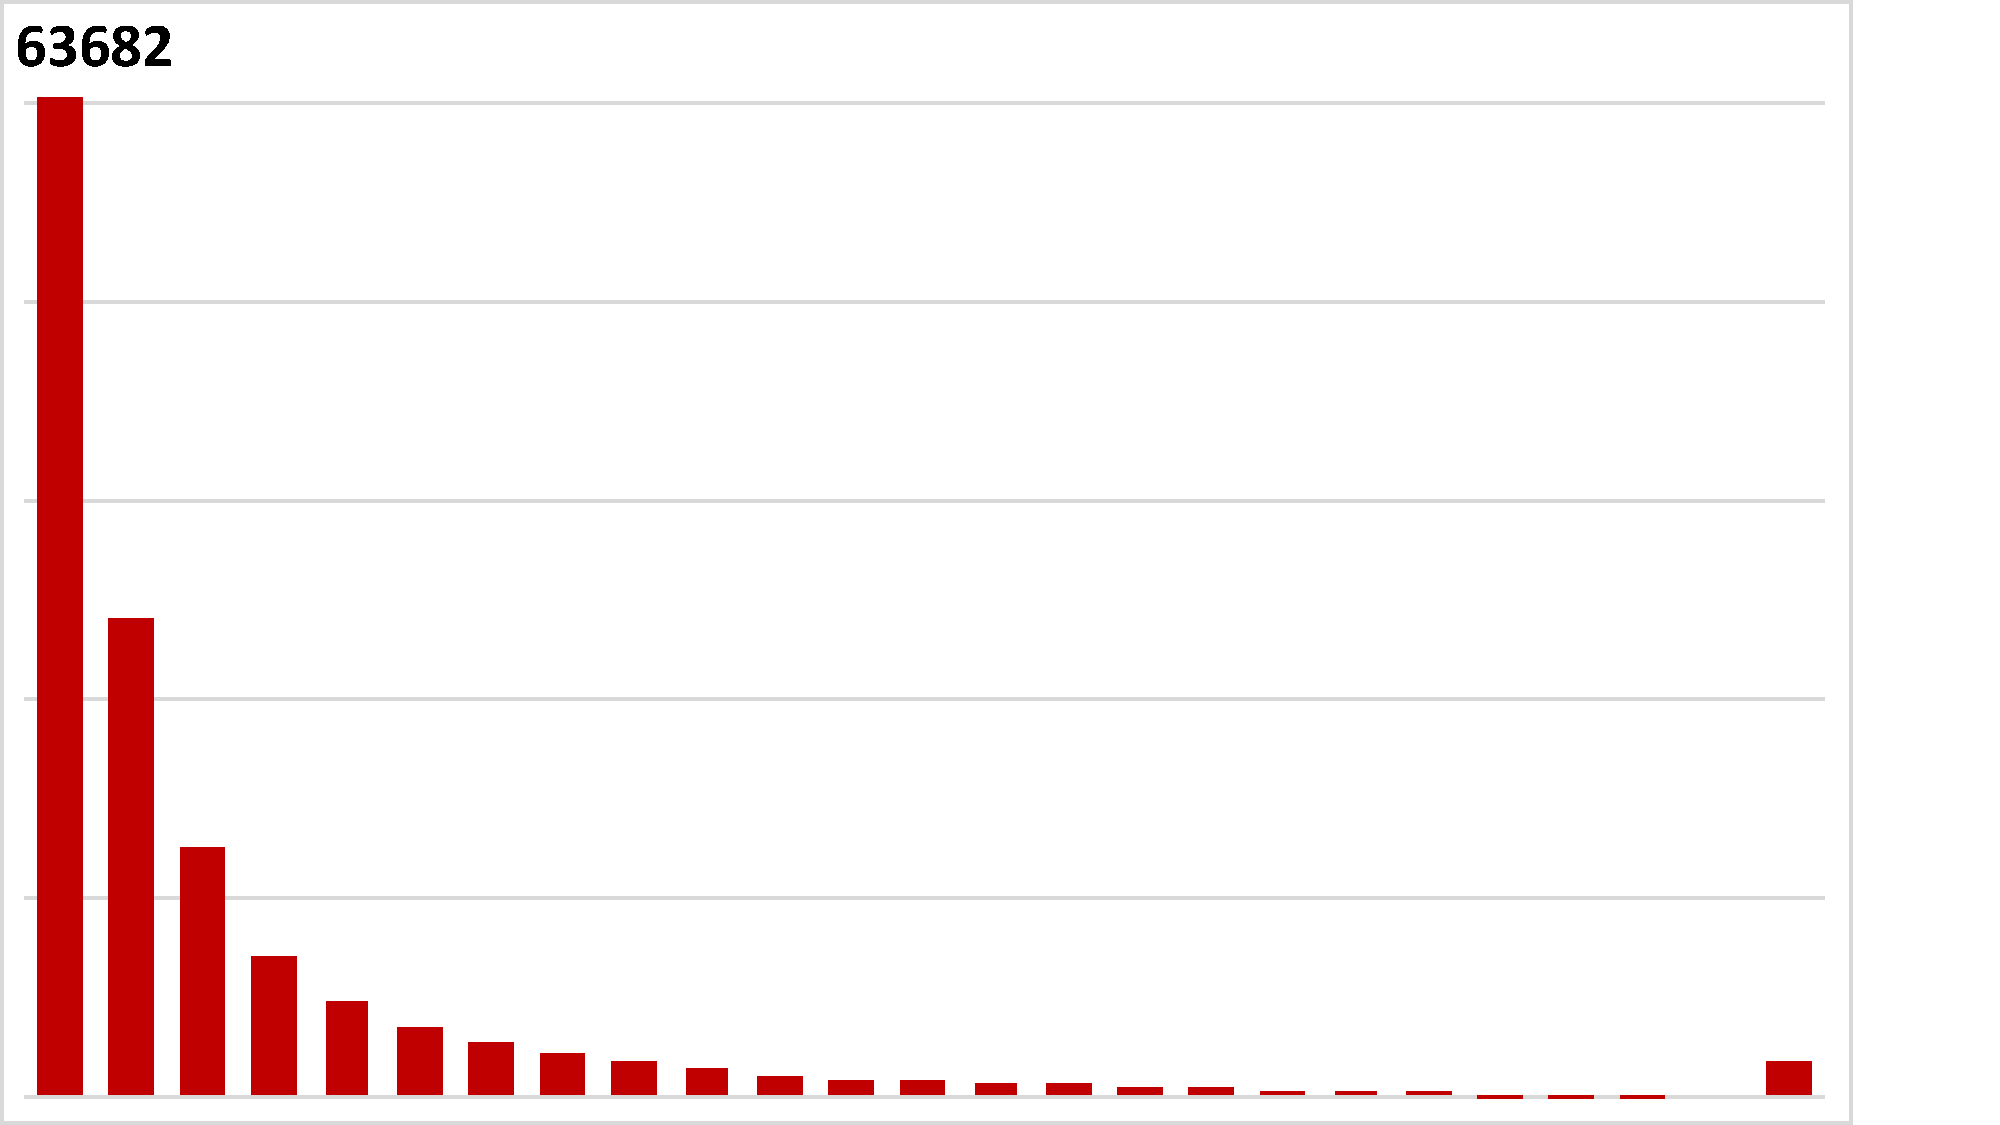
\includegraphics[width=0.9\linewidth, trim={0cm 0cm 2.5cm 0cm}, clip]{results/cloverleaf3d/lag_5/Lag5_AvgL2.pdf}
\vspace{-2mm}
\caption{Lag 40 1:27 Avg$_{L2}$ }
\end{subfigure}
\begin{subfigure}{0.195\textwidth}
\centering
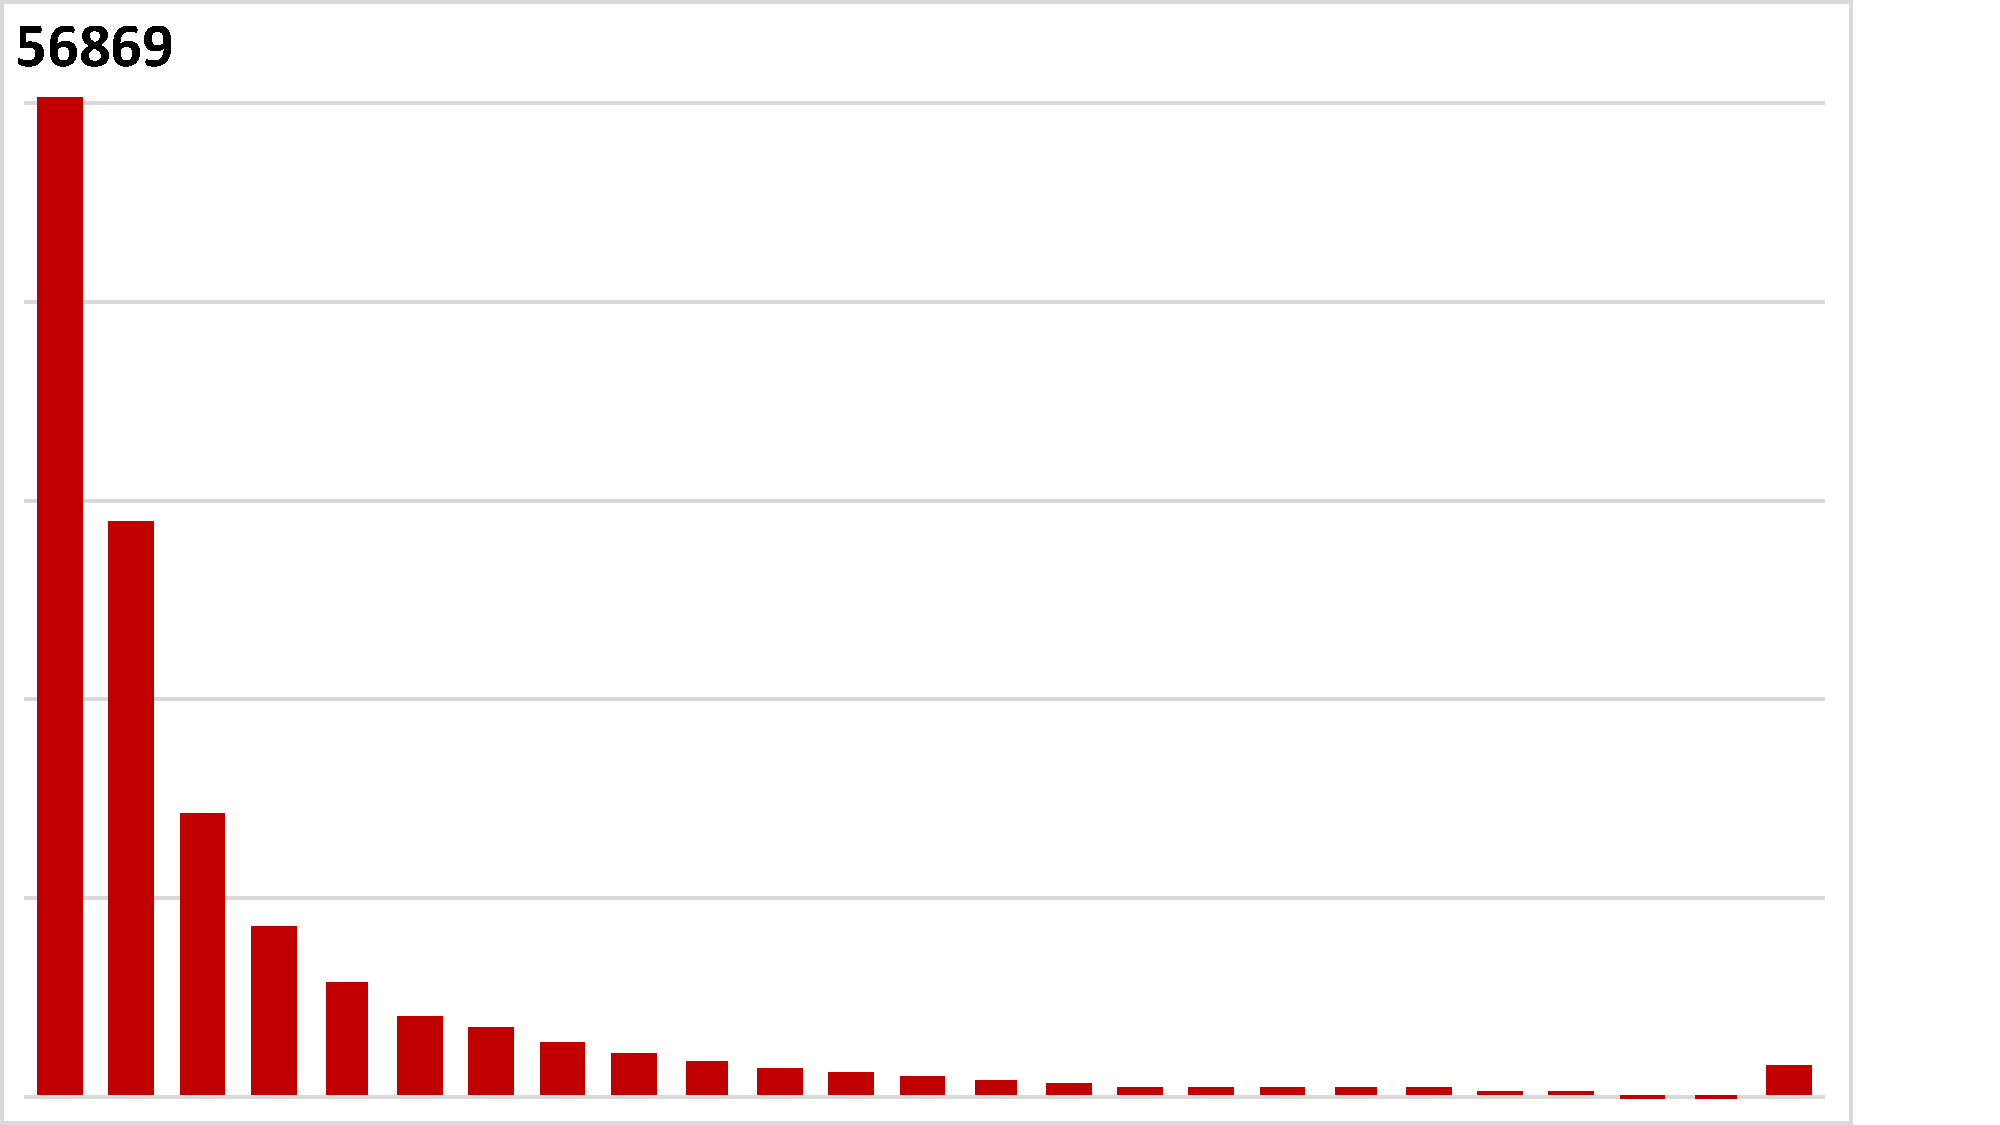
\includegraphics[width=0.9\linewidth, trim={0cm 0cm 2.5cm 0cm}, clip]{results/cloverleaf3d/lag_6/Lag6_AvgL2.pdf}
\vspace{-2mm}
\caption{Lag 40 1:64 Avg$_{L2}$ }
\end{subfigure}
\begin{subfigure}{0.195\textwidth}
\centering
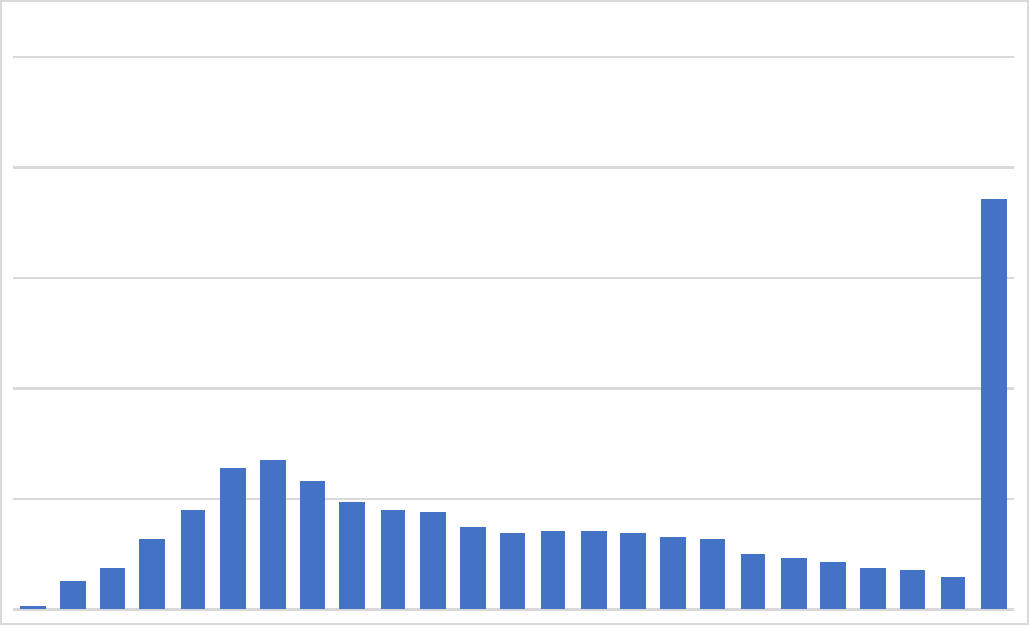
\includegraphics[width=0.9\linewidth]{results/cloverleaf3d/eul_1/Eul1_Max.pdf}
\vspace{-2mm}
\caption{Eul 20 Max$_{L2}$ }
\end{subfigure}
\begin{subfigure}{0.195\textwidth}
\centering
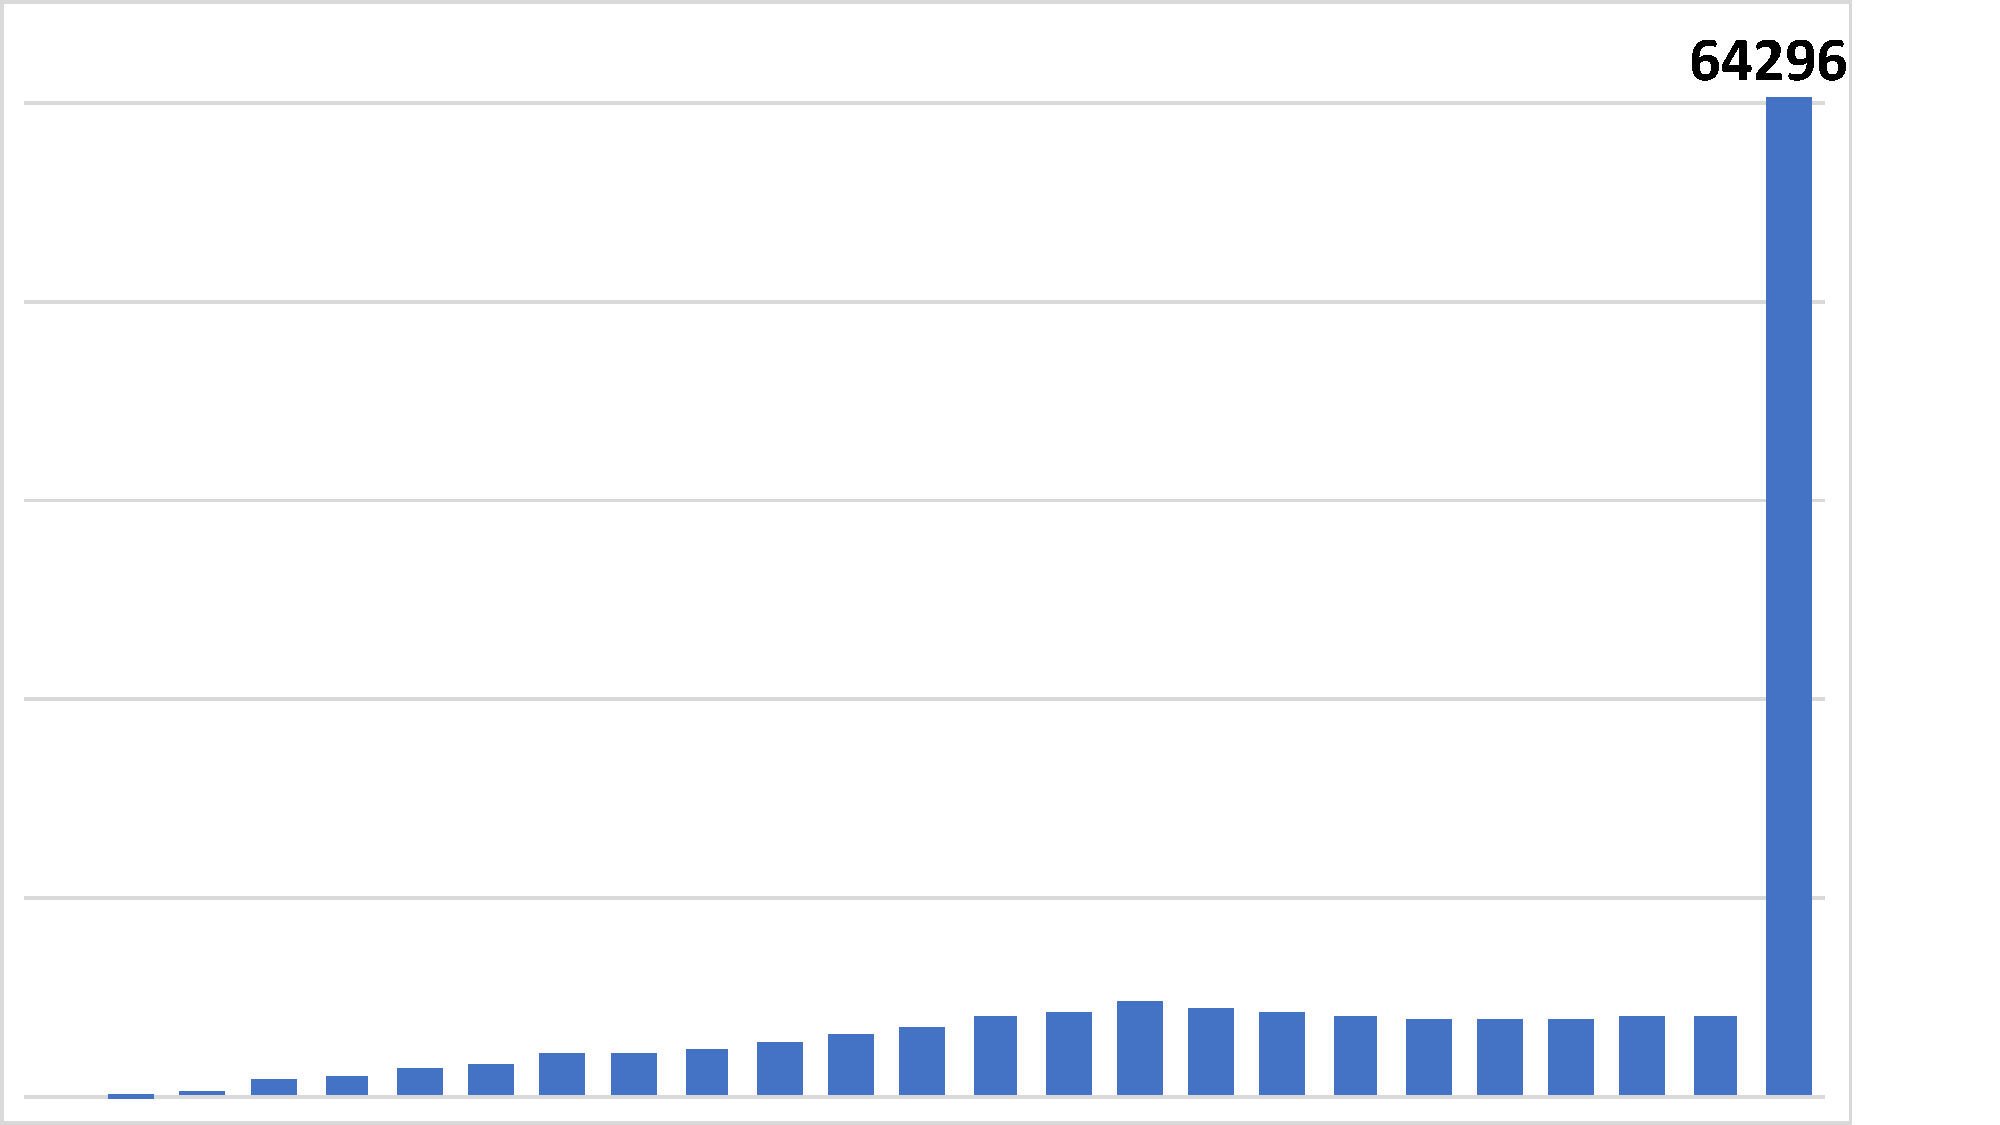
\includegraphics[width=0.95\linewidth]{results/cloverleaf3d/eul_2/Eul2_Max.pdf}
\vspace{-2mm}
\caption{Eul 40 Max$_{L2}$ }
\end{subfigure}
\hspace{0.2mm}
\begin{subfigure}{0.195\textwidth}
\centering
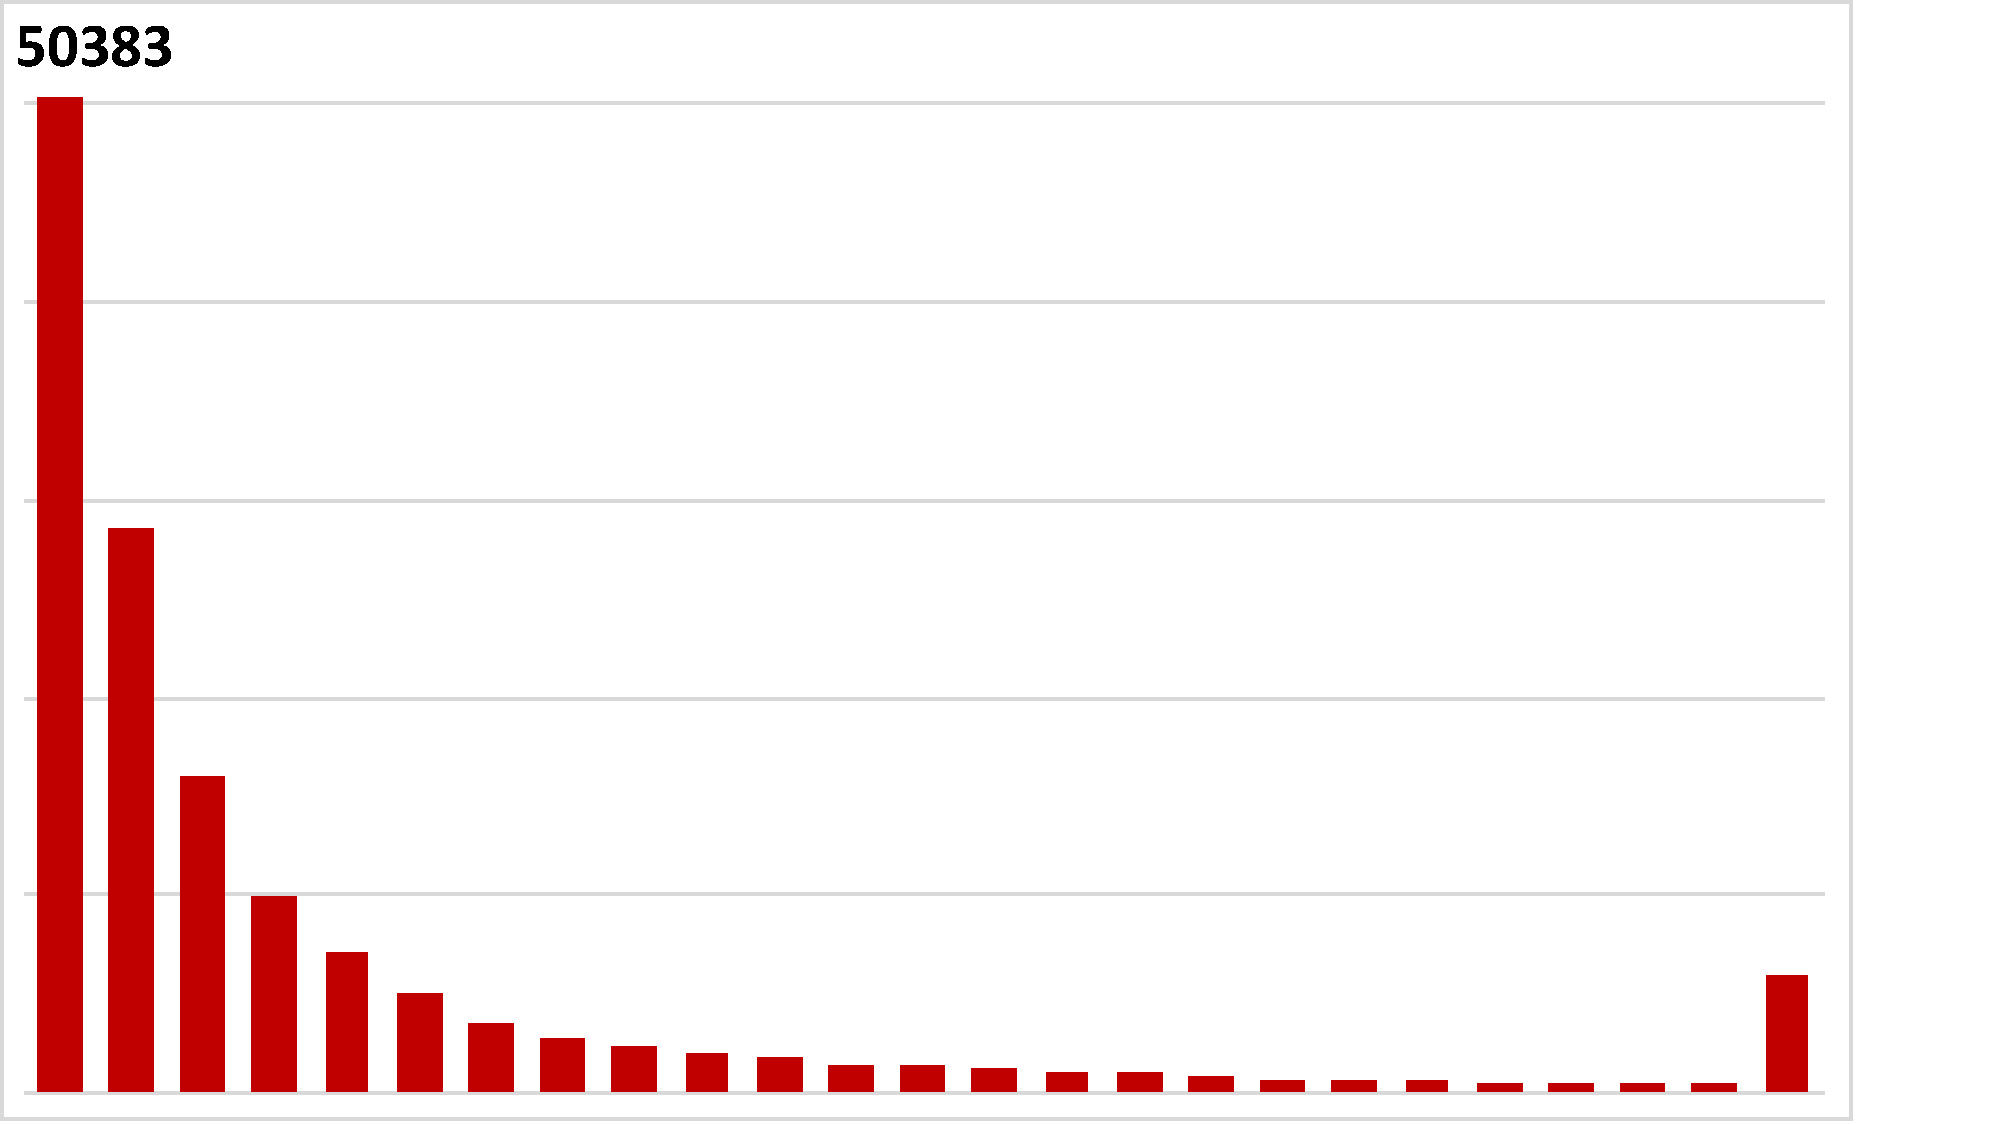
\includegraphics[width=0.9\linewidth, trim={0cm 0cm 2.5cm 0cm}, clip]{results/cloverleaf3d/lag_4/Lag4_Max.pdf}
\vspace{-2mm}
\caption{Lag 40 1:8 Max$_{L2}$ }
\end{subfigure}
\begin{subfigure}{0.195\textwidth}
\centering
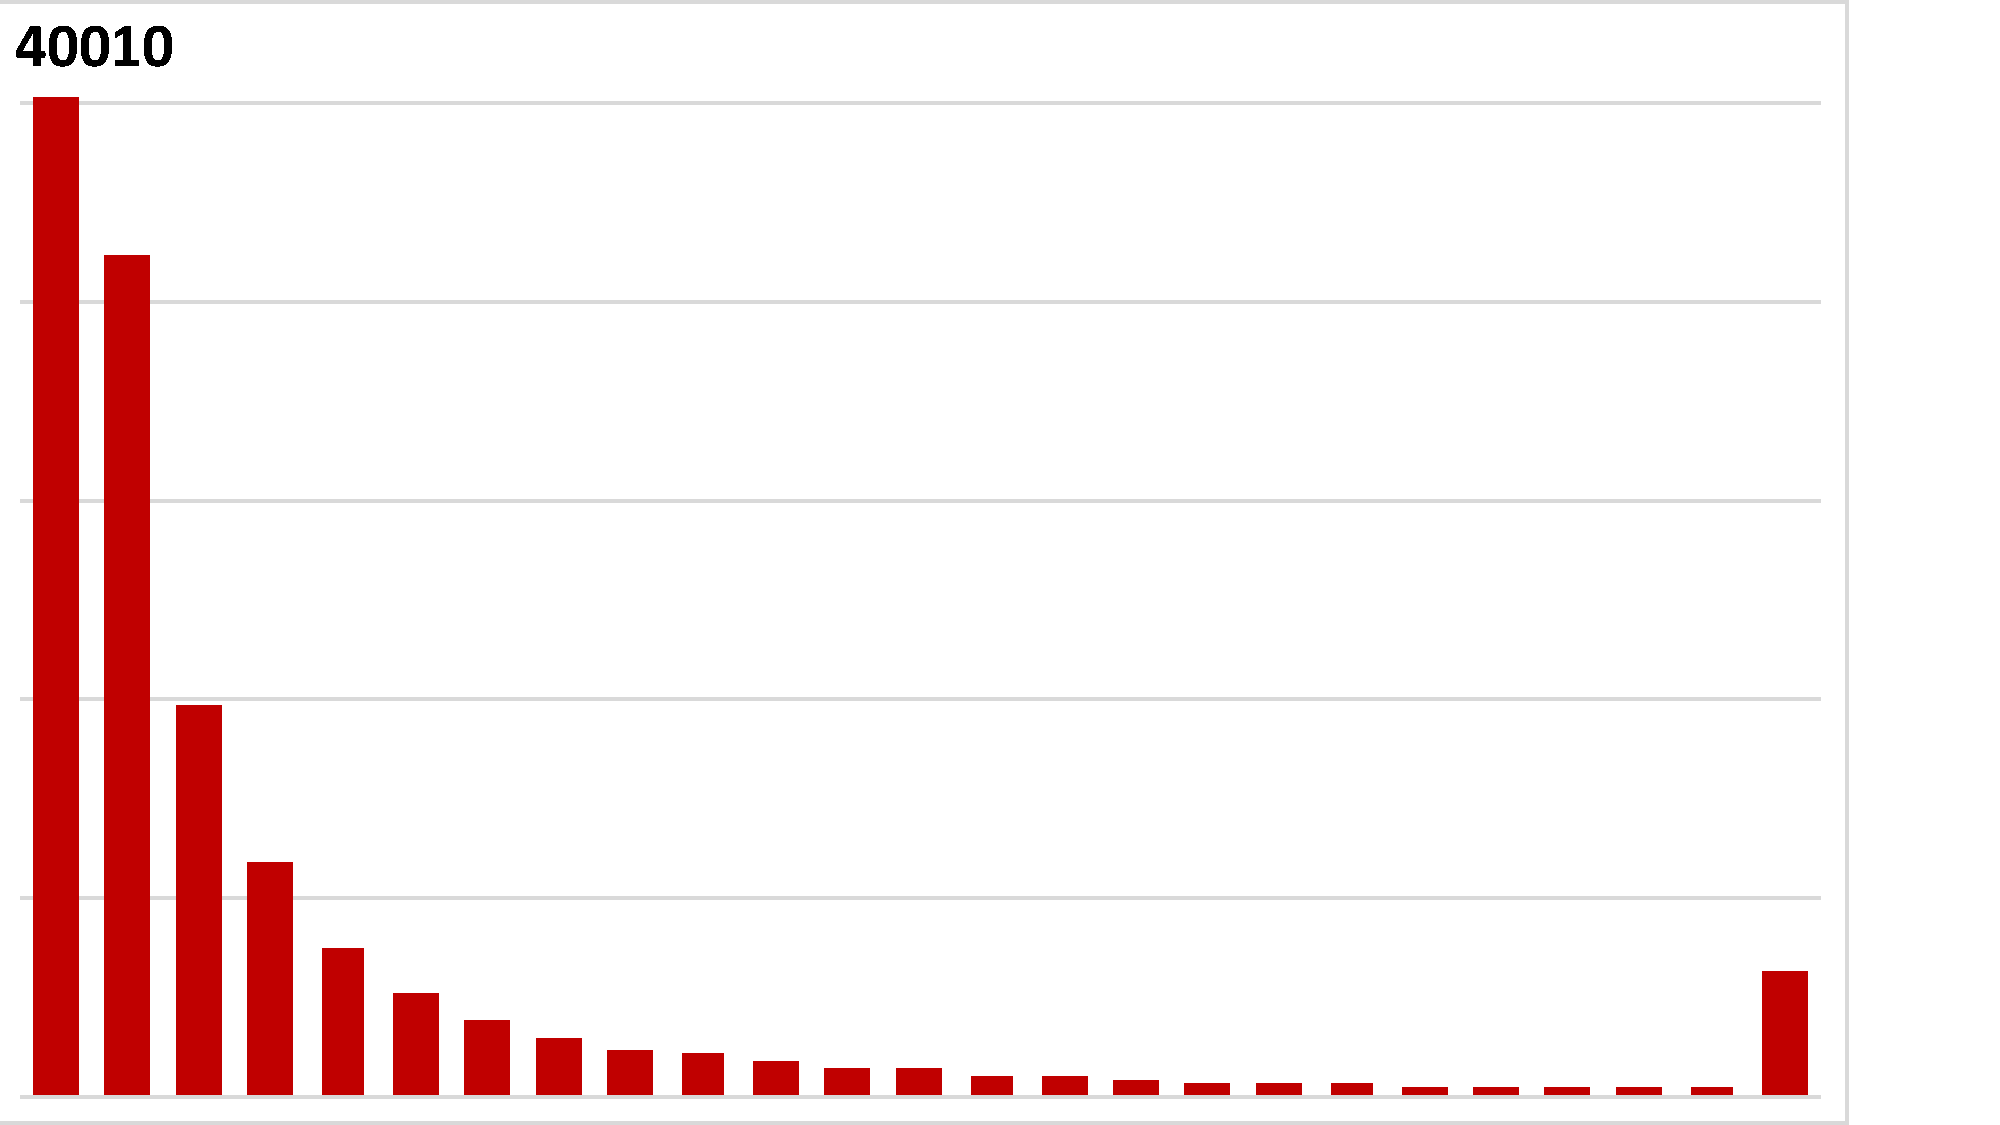
\includegraphics[width=0.9\linewidth, trim={0cm 0cm 2.5cm 0cm}, clip]{results/cloverleaf3d/lag_5/Lag5_Max.pdf}
\vspace{-2mm}
\caption{Lag 40 1:27 Max$_{L2}$}
\end{subfigure}
\begin{subfigure}{0.195\textwidth}
\centering
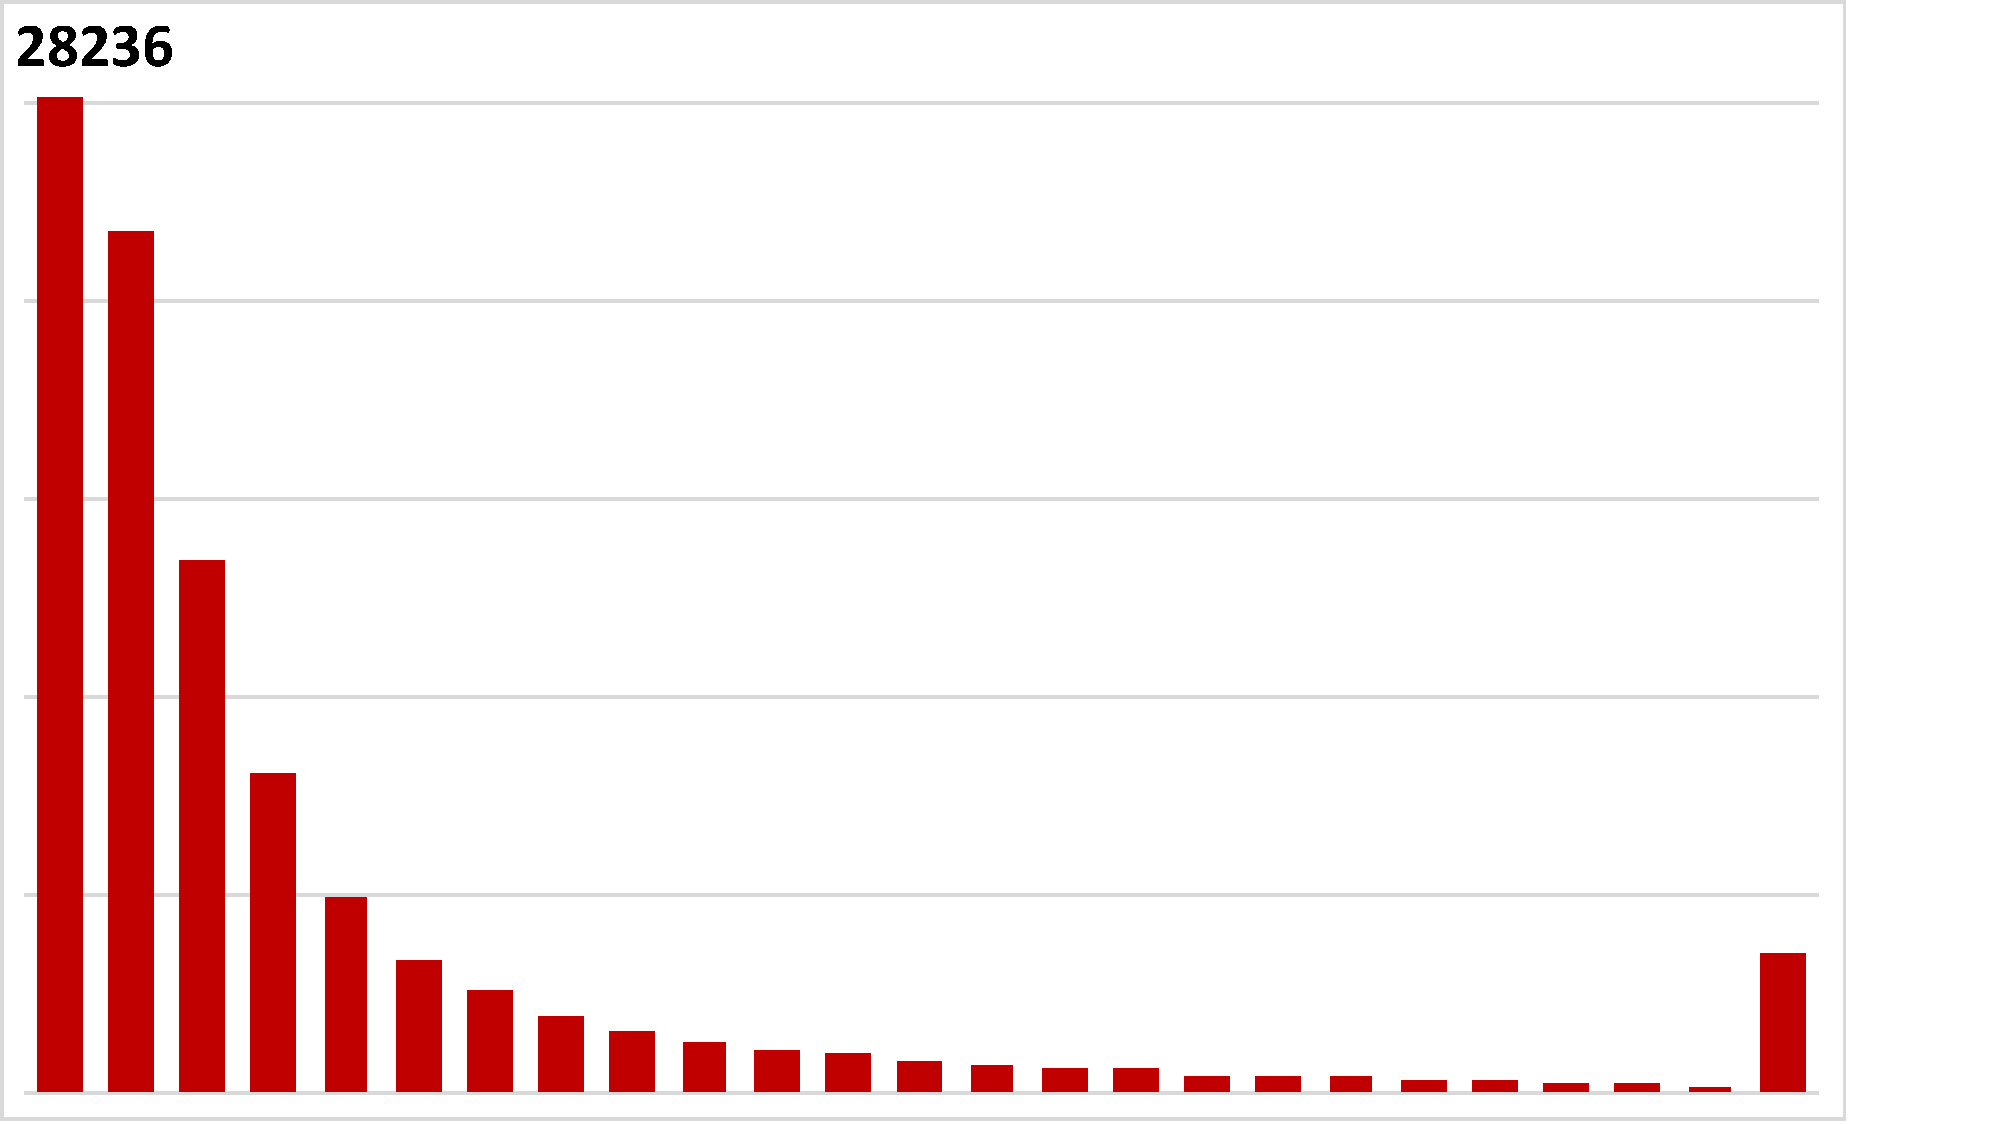
\includegraphics[width=0.9\linewidth, trim={0cm 0cm 2.5cm 0cm}, clip]{results/cloverleaf3d/lag_6/Lag6_Max.pdf}
\vspace{-2mm}
\caption{Lag 40 1:64 Max$_{L2}$}
\end{subfigure}
%\begin{subfigure}{0.24\textwidth}
%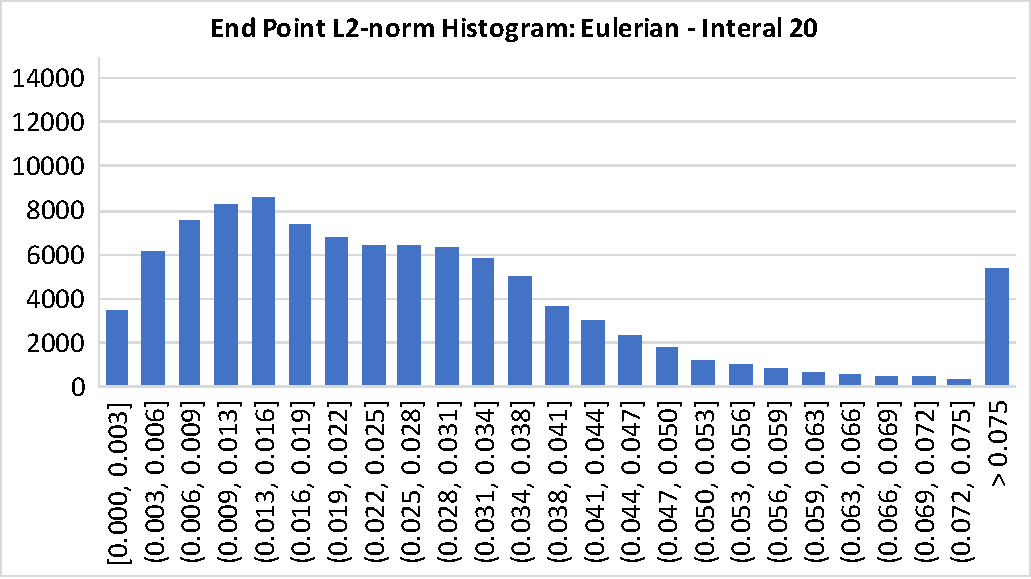
\includegraphics[width=0.9\linewidth]{results/cloverleaf3d/eul_1/Eul1_EndPt.pdf}
%\caption{Eulerian 20 End Point}
%\end{subfigure}
%\hspace{1mm}
%\begin{subfigure}{0.21\textwidth}
%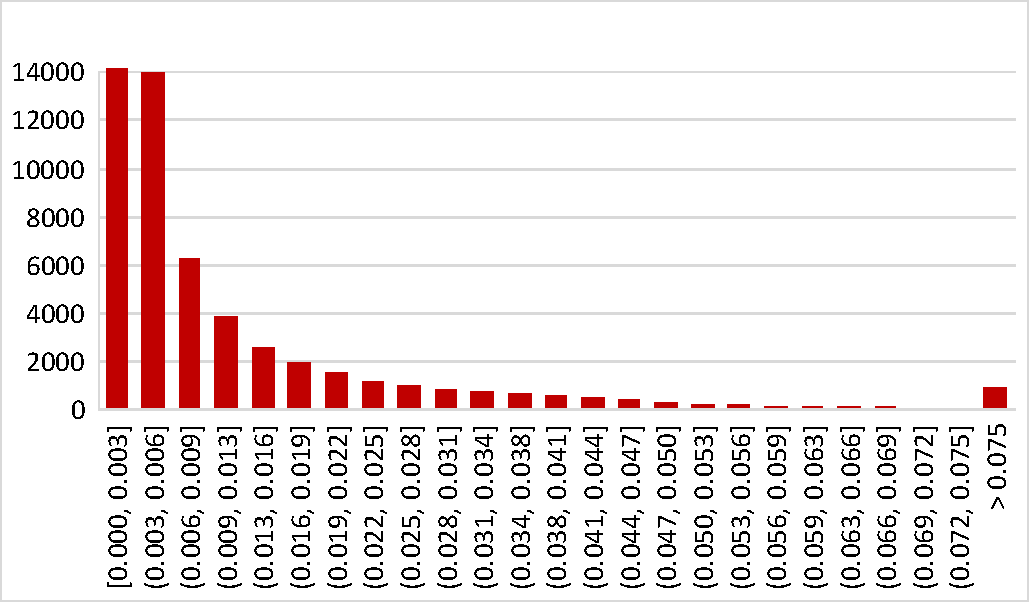
\includegraphics[width=1\linewidth]{results/cloverleaf3d/lag_4/Lag4_EndPt.pdf}
%\caption{Lagrangian 40 1:8 End Point}
%\end{subfigure}
%\hspace{1mm}
%\begin{subfigure}{0.21\textwidth}
%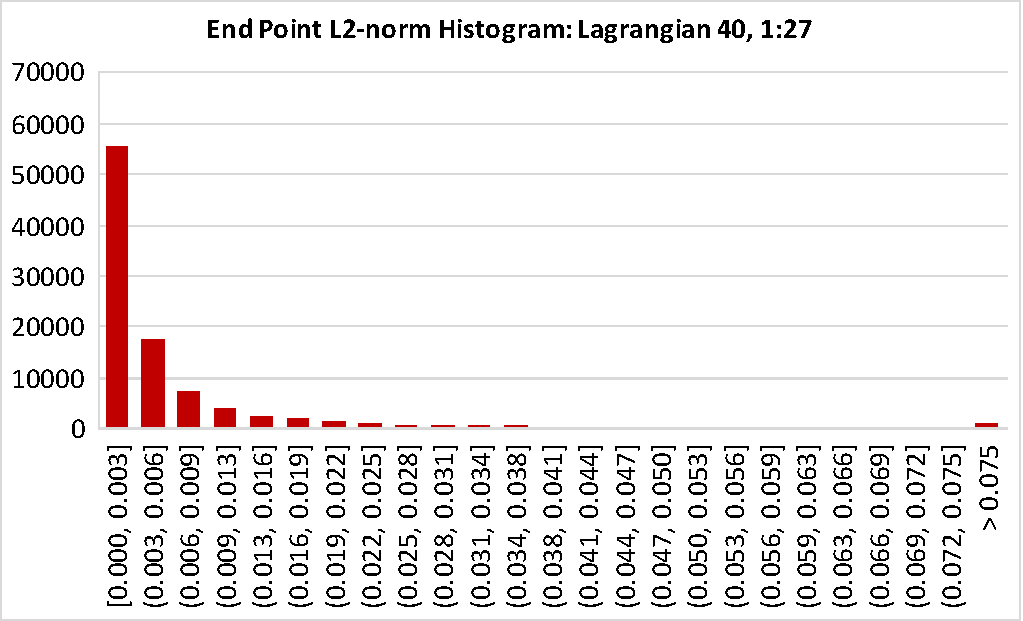
\includegraphics[width=1\linewidth]{results/cloverleaf3d/lag_5/Lag5_EndPt.pdf}
%\caption{Lagrangian 40 1:27 End Point}
%\end{subfigure}
%\hspace{1mm}
%\begin{subfigure}{0.21\textwidth}
%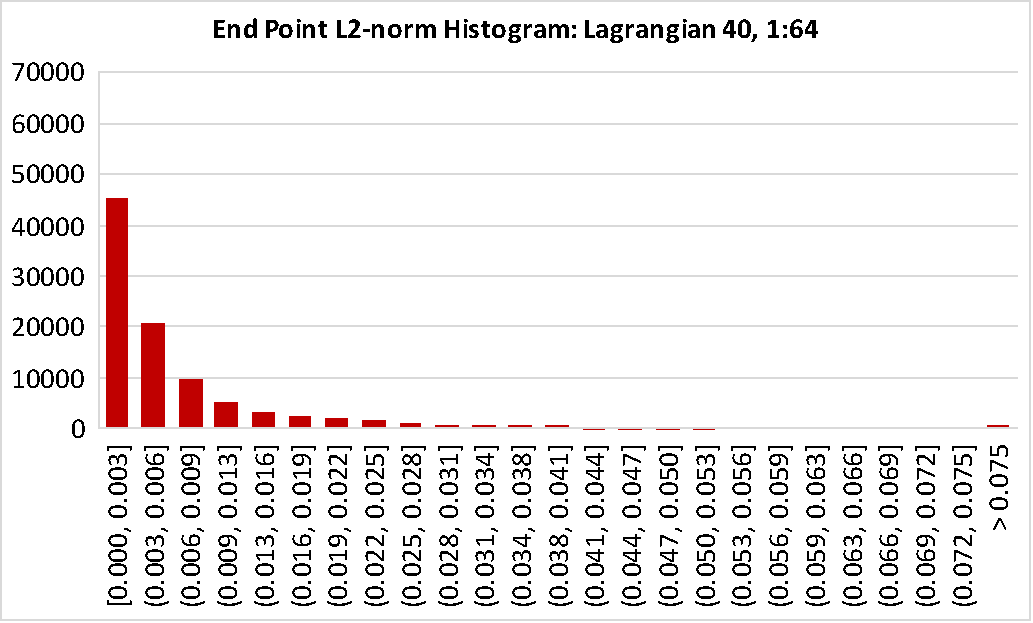
\includegraphics[width=1\linewidth]{results/cloverleaf3d/lag_6/Lag6_EndPt.pdf}
%\caption{Lagrangian 40 1:64 End Point}
%\end{subfigure}
\vspace{-3mm}
\caption{\textbf{Cloverleaf3D} experiment histograms for 100,000 test particle interpolation errors. Each plot has 25 bins, ranging from 0 to $>$0.05, with bar height encoding number of particles. Horizontal grid lines mark increments of 5,000.} 
\label{fig:clover_histograms}
\vspace{-6mm}
\end{figure*}


%\begin{figure*}
\begin{minipage}[t]{0.33\linewidth}%
\begin{framed}
\setcounter{subfigure}{0}
\begin{minipage}[t]{0.49\textwidth}%
\centering
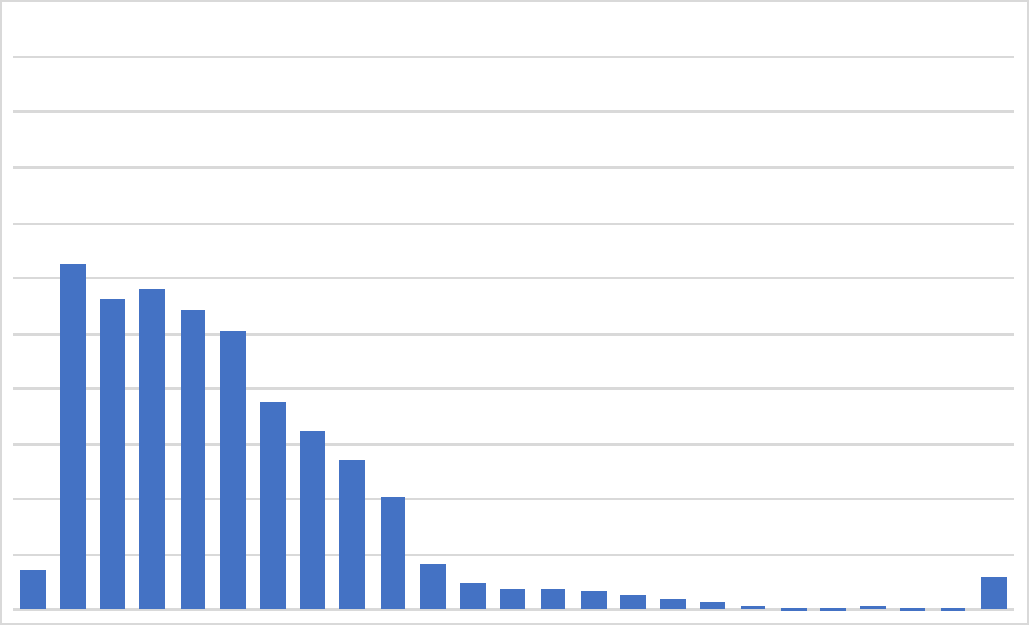
\includegraphics[width=0.95\textwidth]{results/sw4/Eul1_AvgL2.pdf}%
\vspace{-3mm}
\captionof{subfigure}{\footnotesize{Eul 250 Avg$_{L2}$}}
\end{minipage}%
\hfill
\begin{minipage}[t]{0.49\textwidth}%
\centering
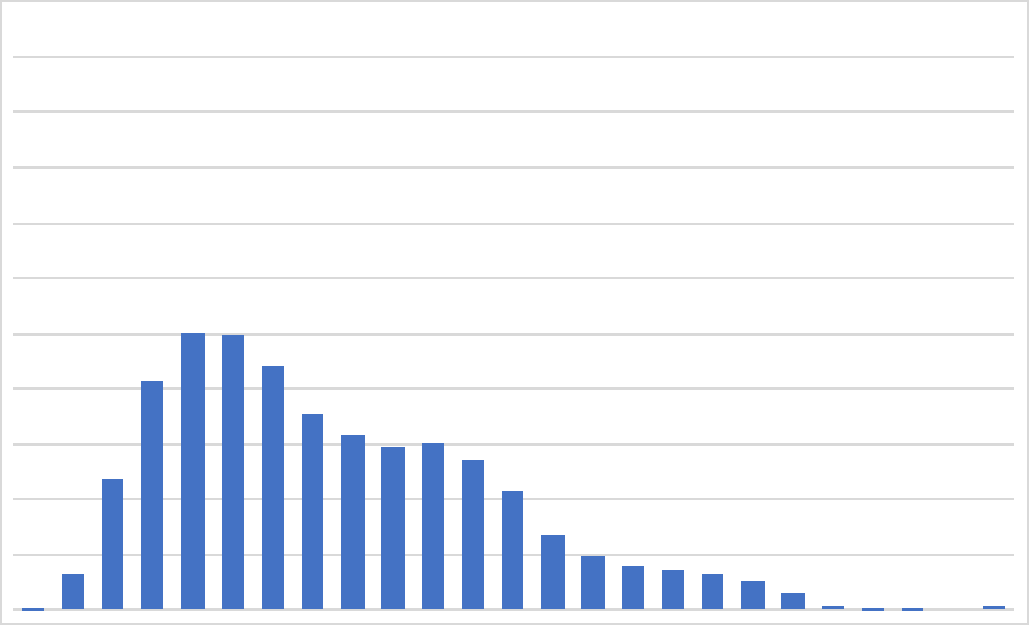
\includegraphics[width=0.95\linewidth]{results/sw4/Eul2_AvgL2.pdf}
\vspace{-3mm}
\captionof{subfigure}{\footnotesize{Eul 500 Avg$_{L2}$}} 
\end{minipage}
\begin{minipage}[t]{0.49\textwidth}%
\centering
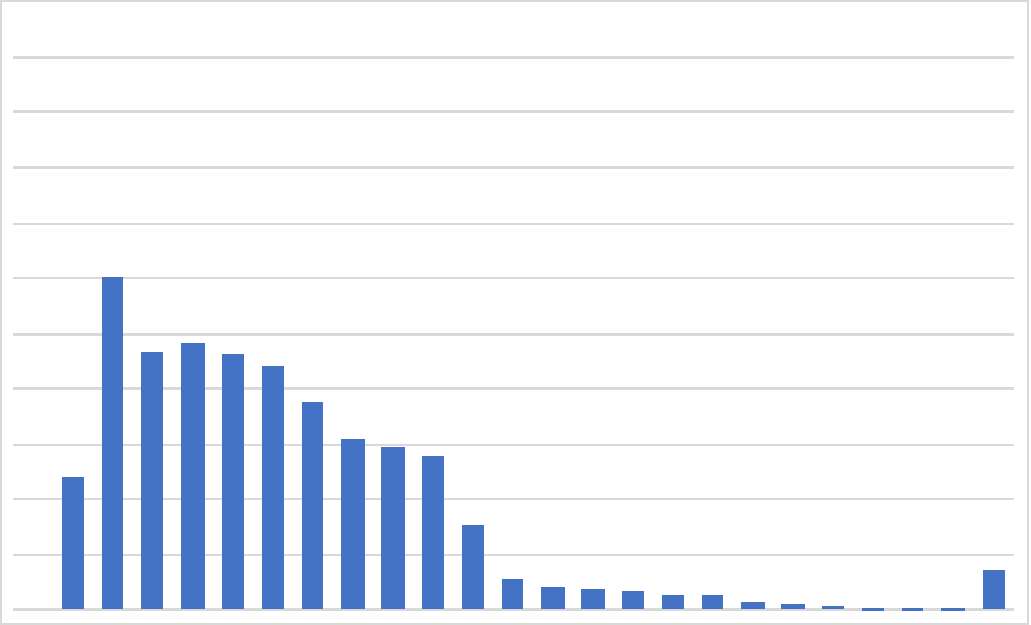
\includegraphics[width=0.95\textwidth]{results/sw4/Eul1_Max.pdf}%
\vspace{-3mm}
\captionof{subfigure}{\footnotesize{Eul 250 Max$_{L2}$}}
\end{minipage}%
\hfill
\begin{minipage}[t]{0.49\textwidth}%
\centering
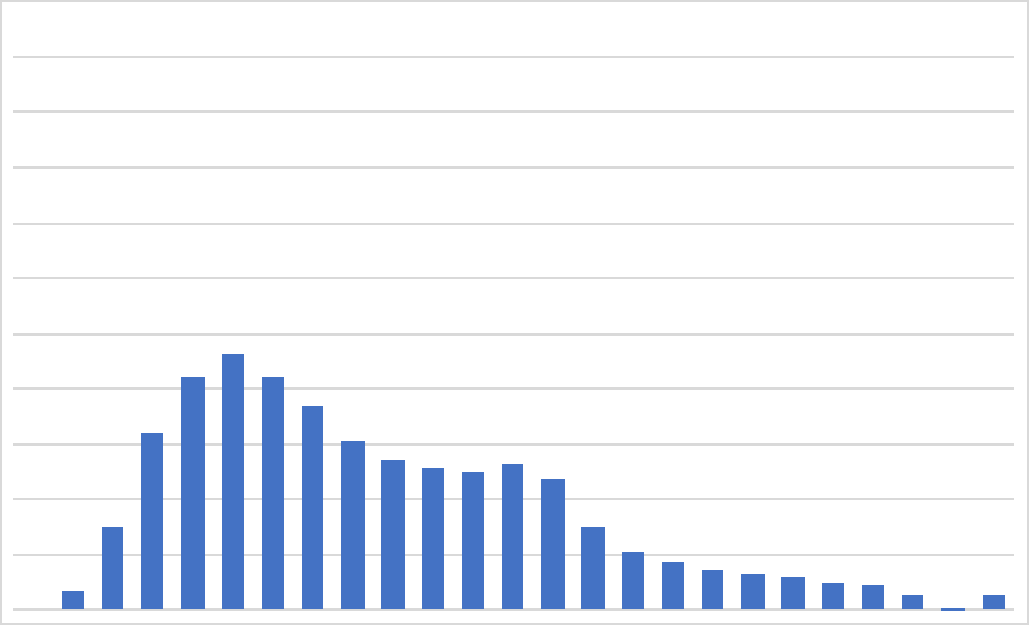
\includegraphics[width=0.95\linewidth]{results/sw4/Eul2_Max.pdf}
\vspace{-3mm}
\captionof{subfigure}{\footnotesize{Eul 500 Max$_{L2}$}} 
\end{minipage}
\begin{minipage}[t]{0.49\textwidth}%
\centering
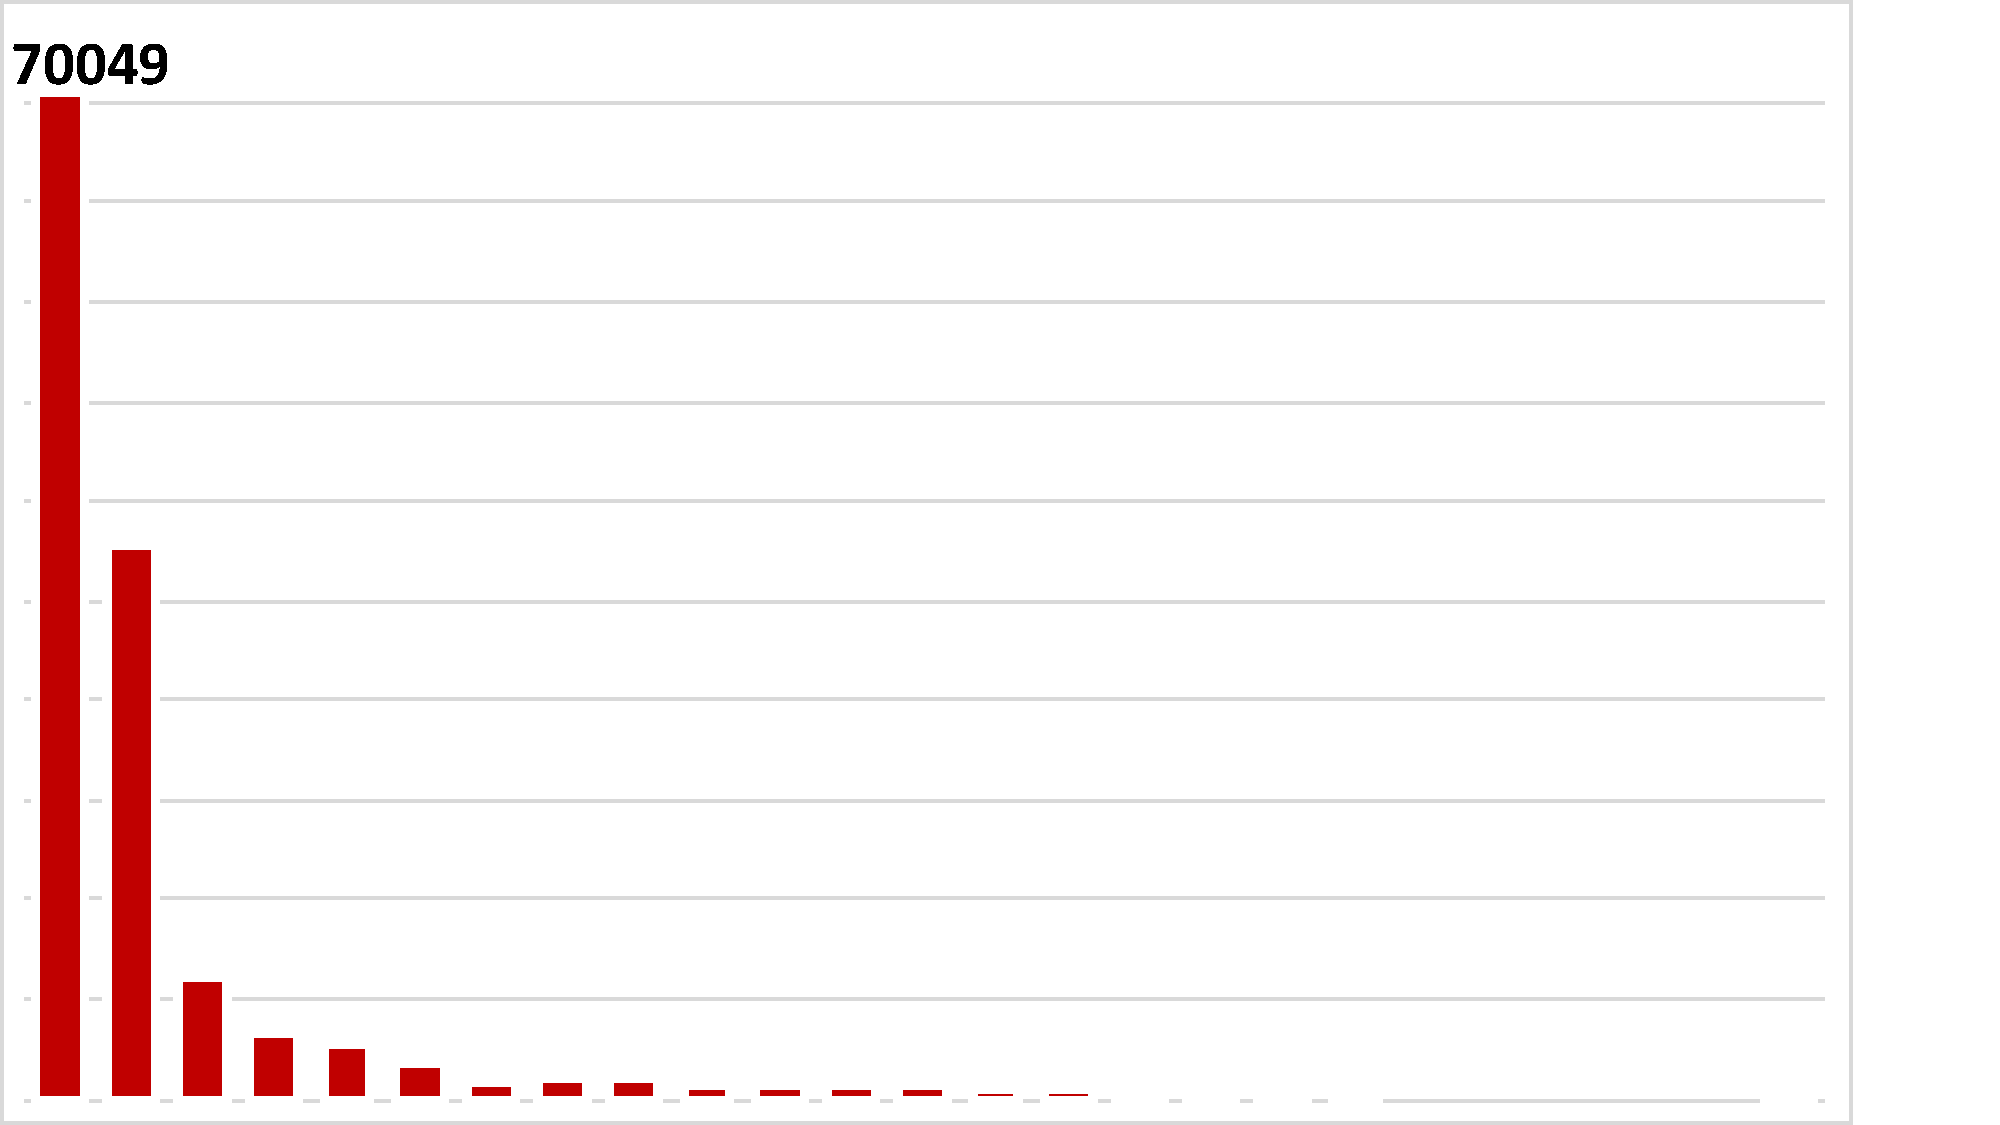
\includegraphics[width=0.95\linewidth, trim={0cm 0cm 2.5cm 0cm}, clip]{results/sw4/Lag3_AvgL2.pdf}
\vspace{-3mm}
\captionof{subfigure}{\footnotesize{Lag 250 1:27 Avg$_{L2}$}}
\end{minipage}%
\hfill
\begin{minipage}[t]{0.49\textwidth}%
\centering
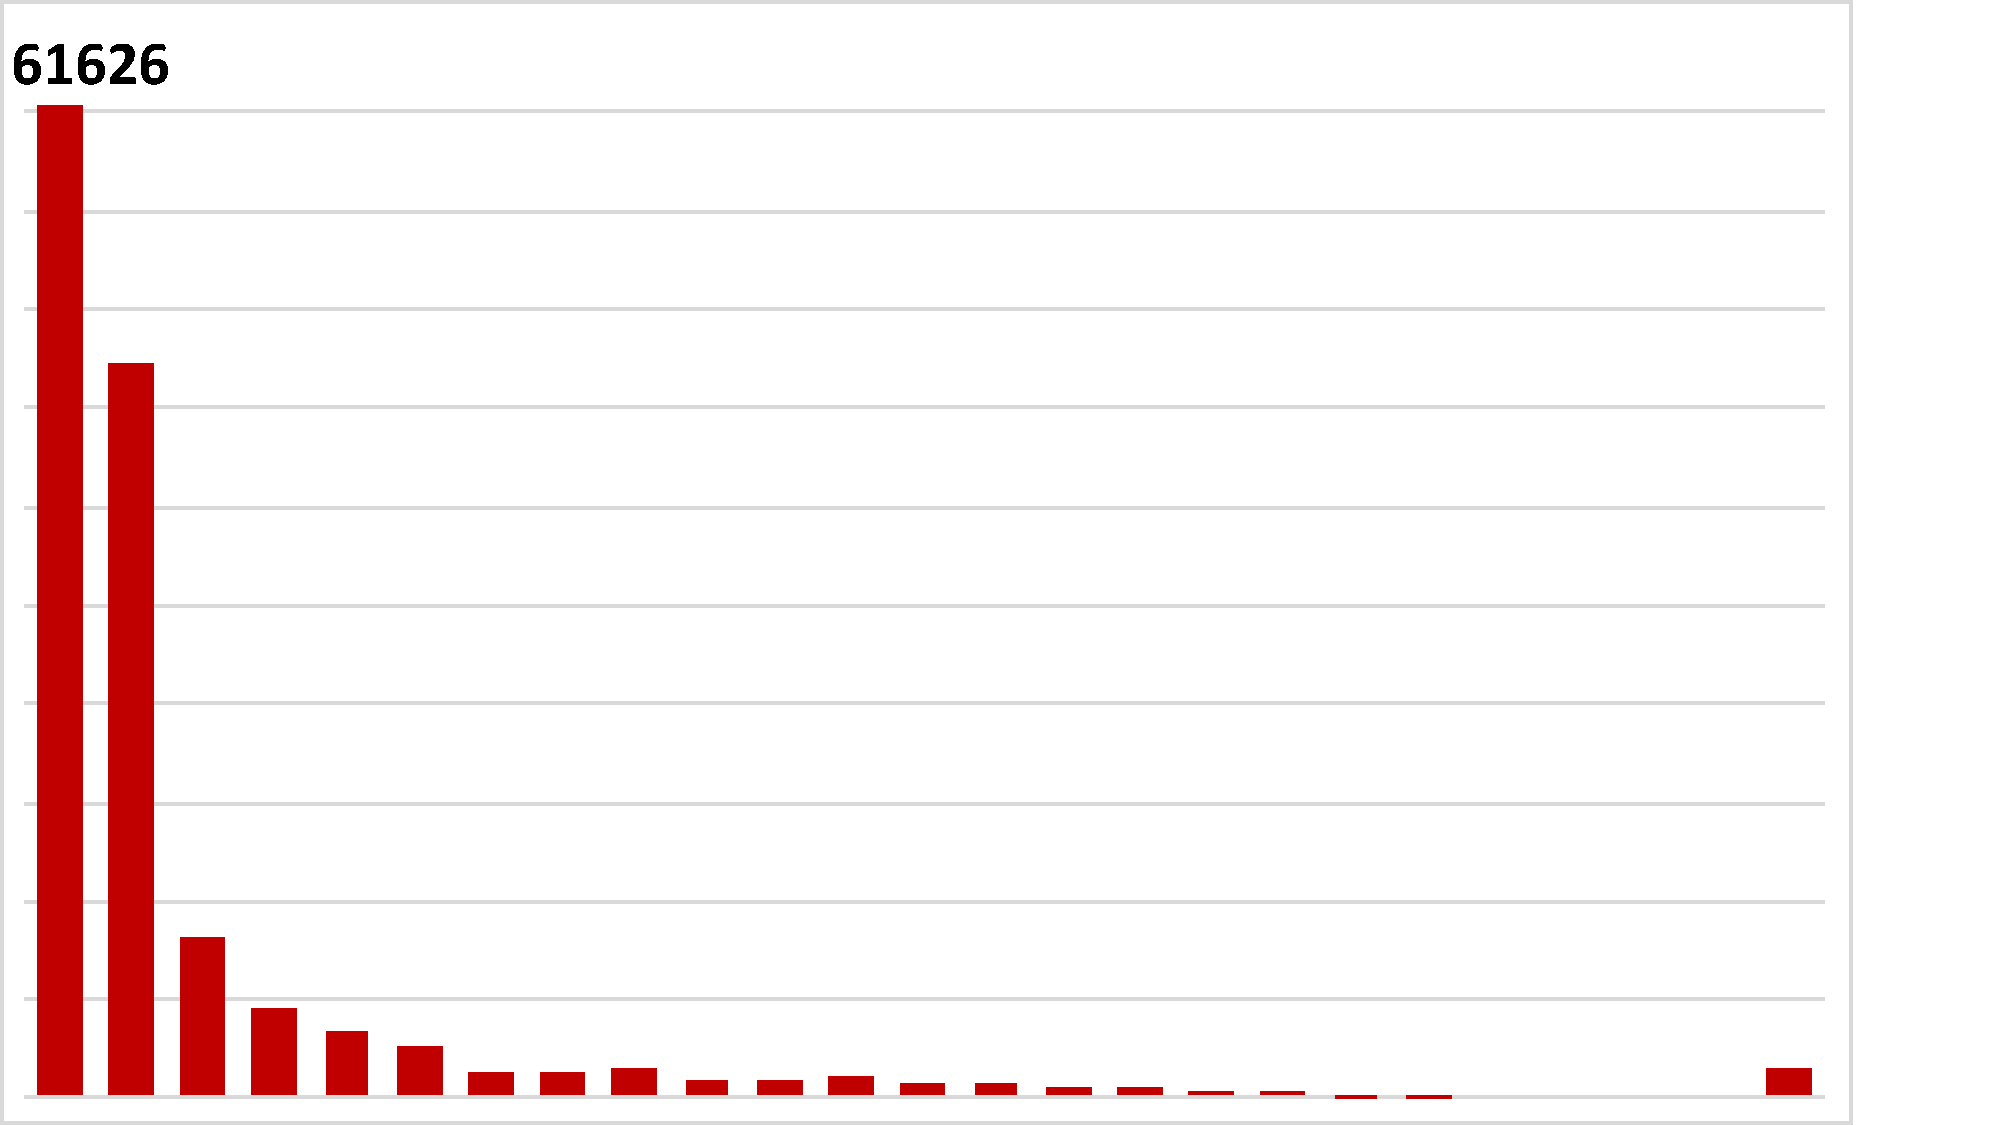
\includegraphics[width=0.95\linewidth, trim={0cm 0cm 2.5cm 0cm}, clip]{results/sw4/Lag4_AvgL2.pdf}
\vspace{-3mm}
\captionof{subfigure}{\footnotesize{Lag 250 1:64 Avg$_{L2}$}} 
\end{minipage}
\begin{minipage}[t]{0.49\textwidth}%
\centering
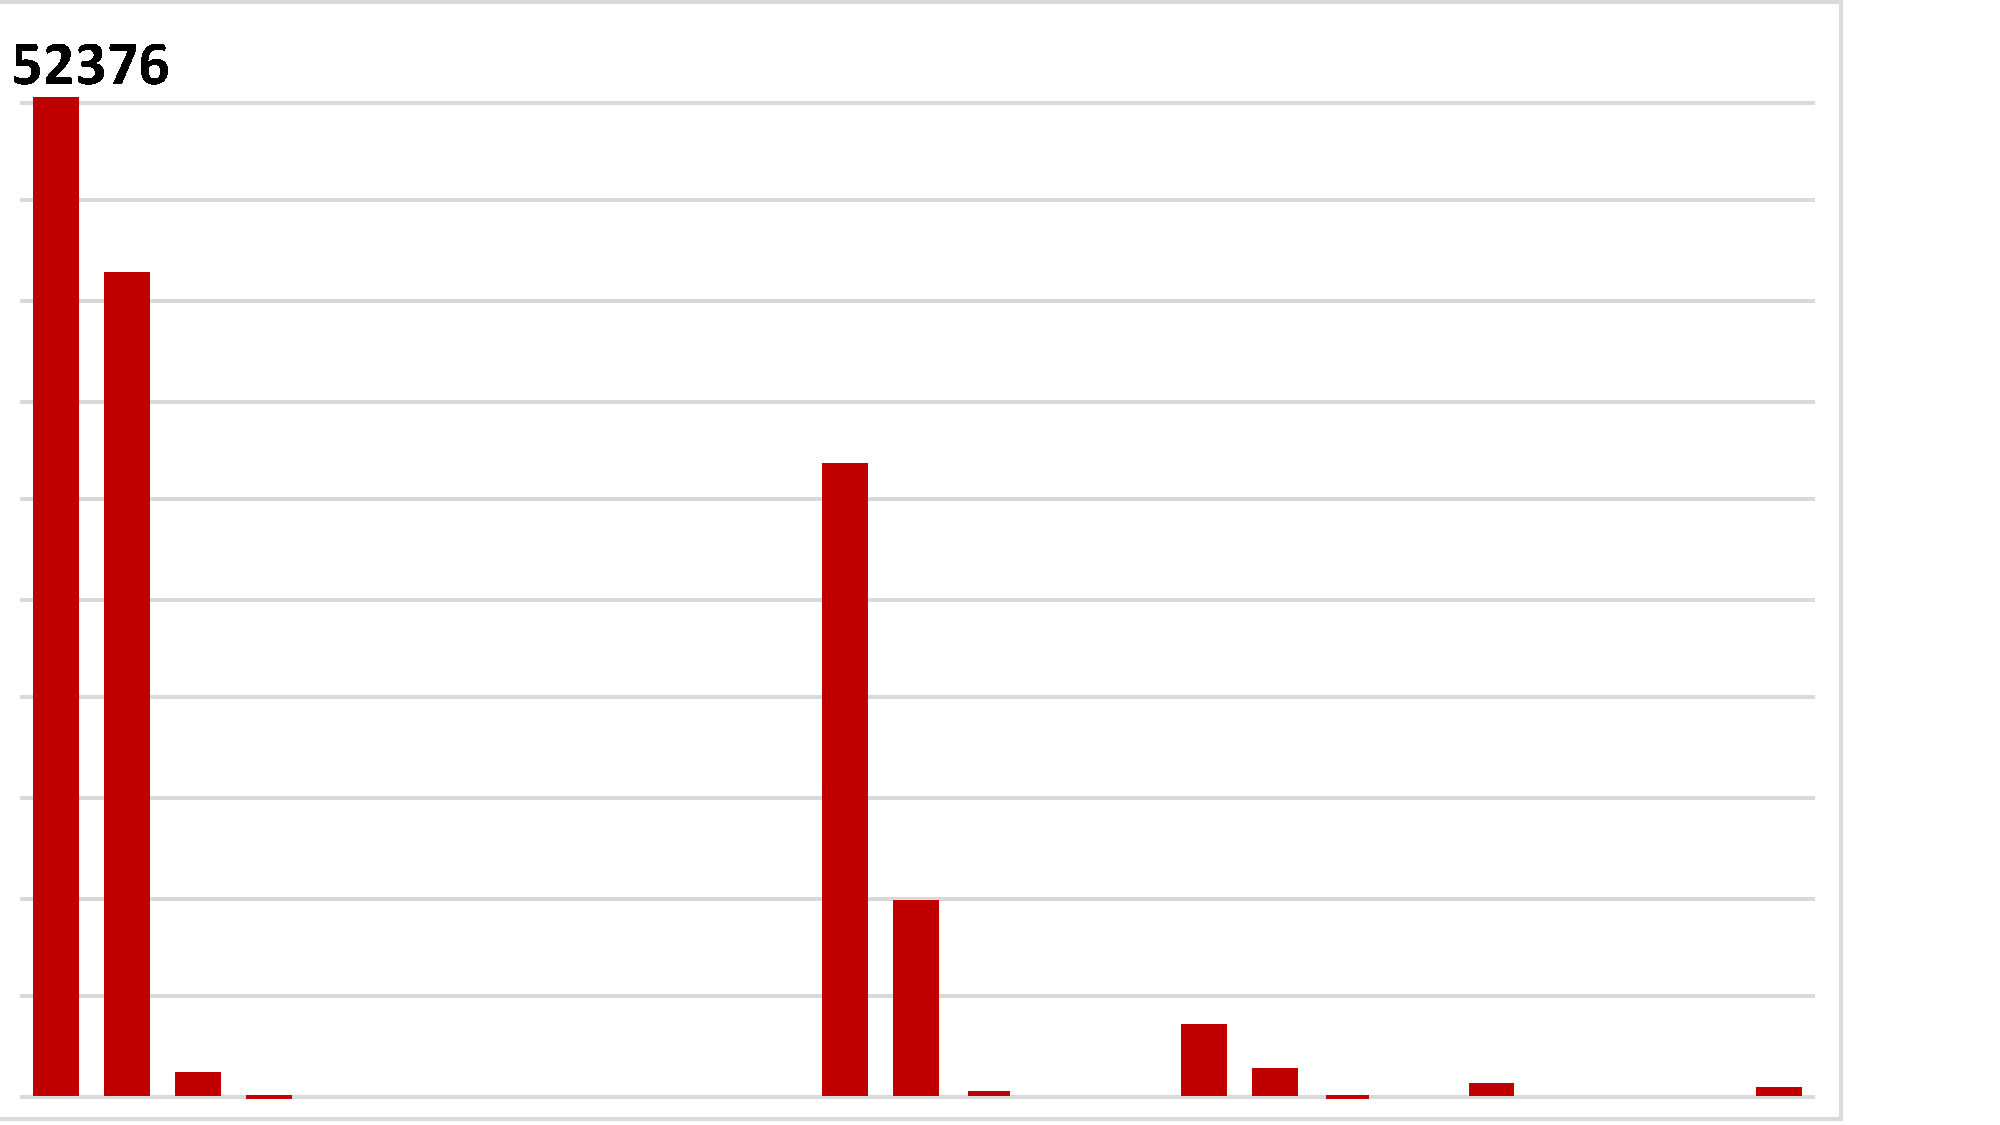
\includegraphics[width=0.95\linewidth, trim={0cm 0cm 2.5cm 0cm}, clip]{results/sw4/Lag3_Max.pdf}
\vspace{-3mm}
\captionof{subfigure}{\footnotesize{Lag 250 1:27 Max$_{L2}$}}
\end{minipage}%
\hfill
\begin{minipage}[t]{0.49\textwidth}%
\centering
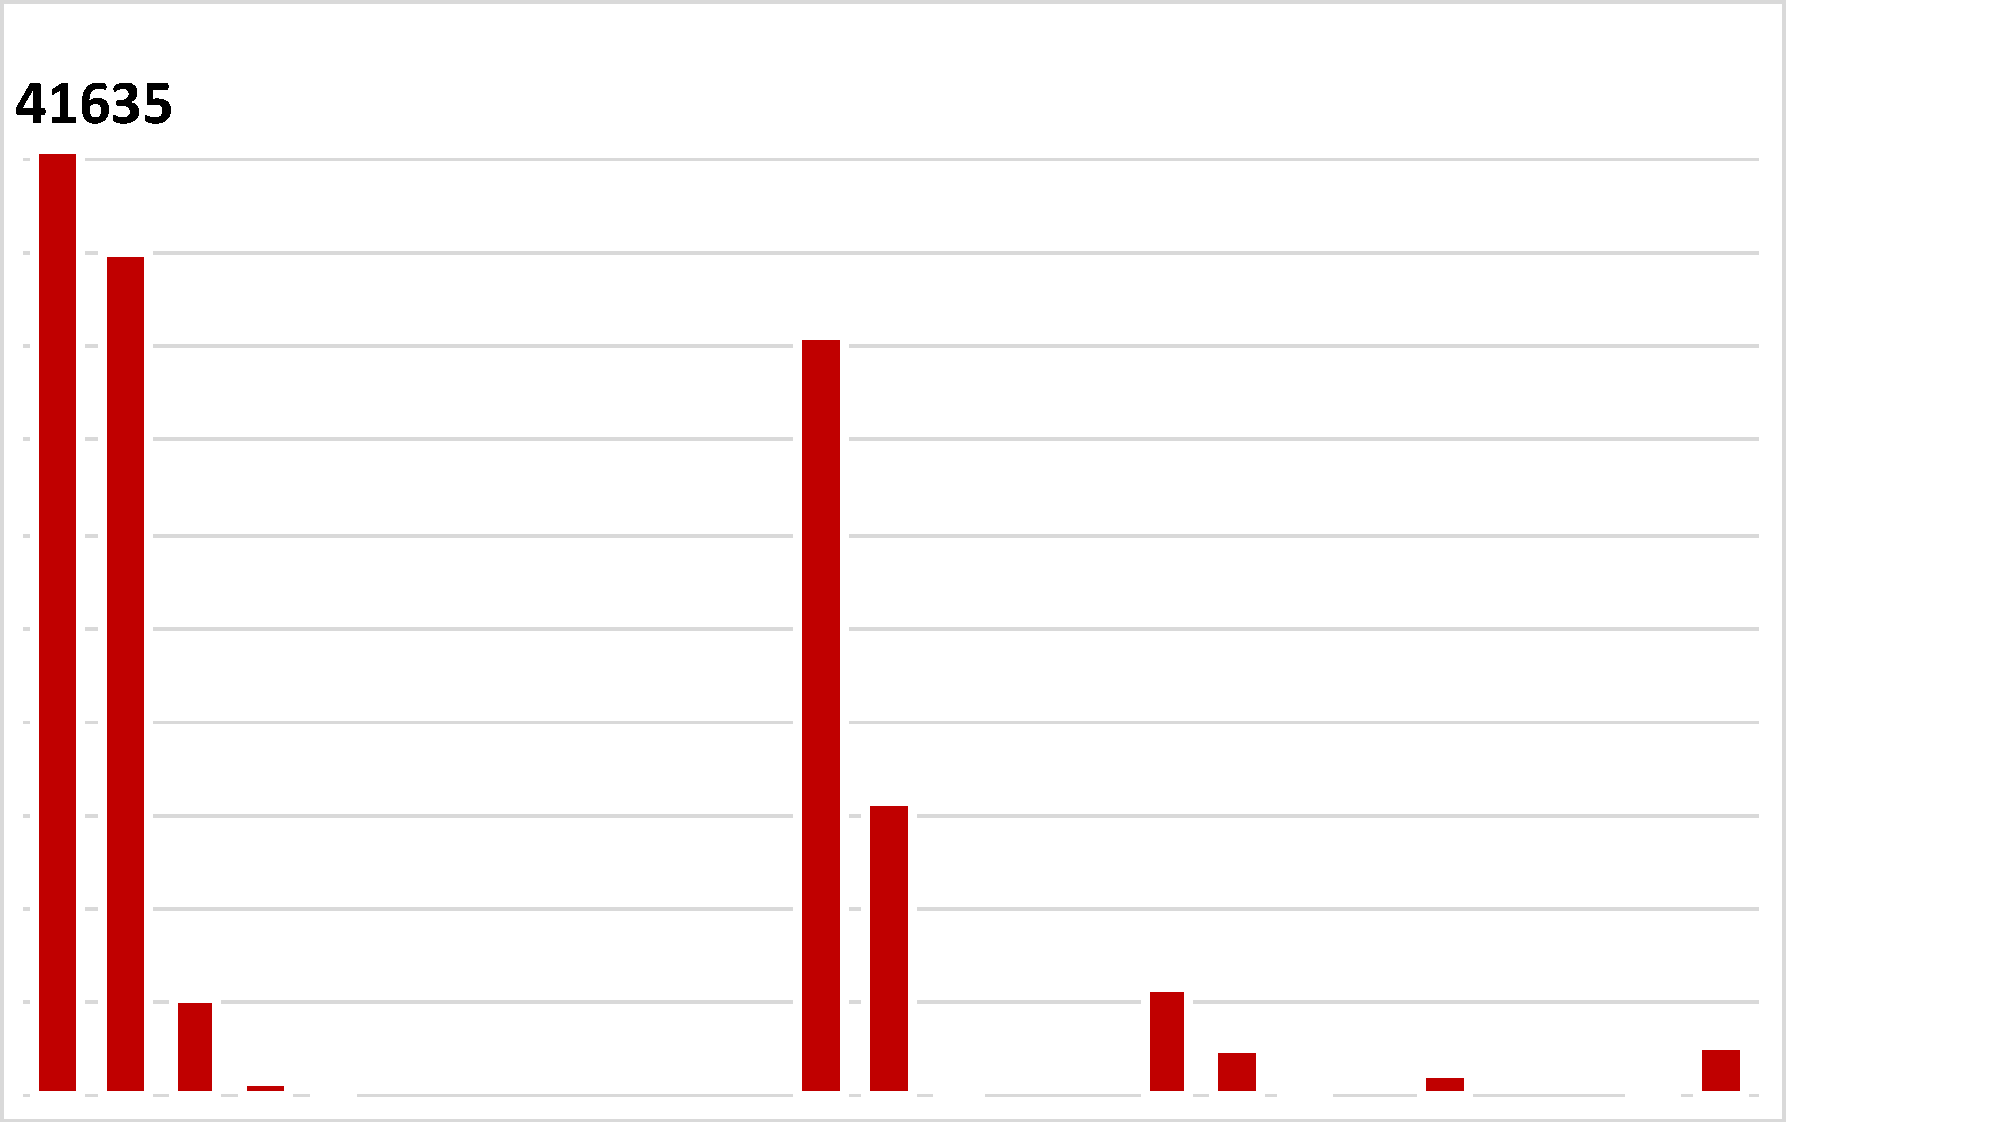
\includegraphics[width=0.95\linewidth, trim={0cm 0cm 2.5cm 0cm}, clip]{results/sw4/Lag4_Max.pdf}
\vspace{-3mm}
\captionof{subfigure}{\footnotesize{Lag 250 1:64 Max$_{L2}$}} 
\end{minipage}
\end{framed}
\vspace{-2mm}
\captionof{figure}{\textbf{SW4} experiment histograms for 90,000 test particle interpolation errors. Each plot has 25 bins, Eulerian bins range from $<$0.6 to $>$15, Lagrangian bins range from 0 to $>$0.2, with bar height encoding number of particles. Horizontal grid lines mark increments of 2,000.}
\label{fig:sw4_histograms}
\end{minipage}% End of SW4
%%%%%%%%%%%%%%%%%%%%%%%%%%%%%%%%%%%
\setcounter{subfigure}{0}
\hfill
\begin{minipage}[t]{0.66\linewidth}%
\begin{framed}
\begin{minipage}[t]{0.24\textwidth}%
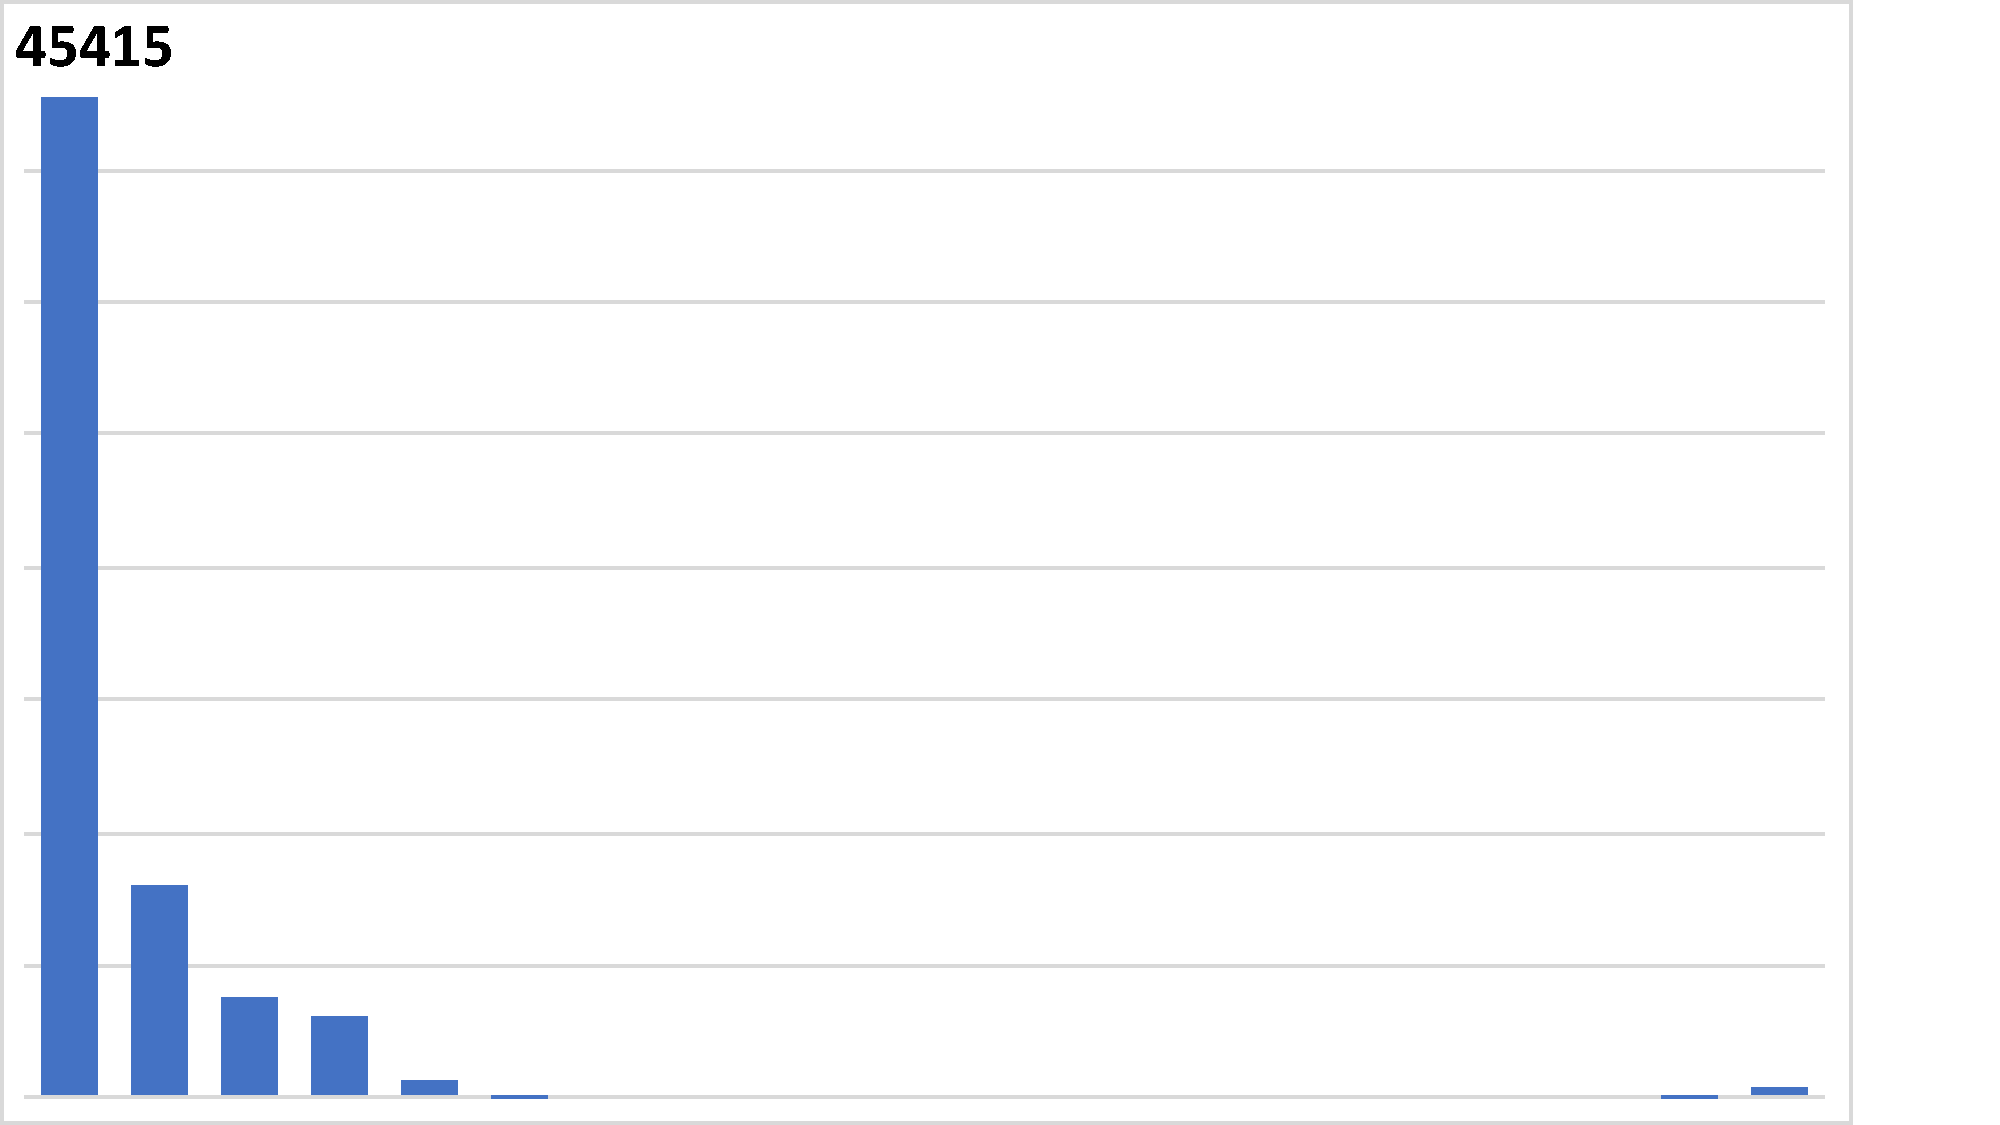
\includegraphics[width=0.95\linewidth, trim={0cm 0cm 2.5cm 0cm}, clip]{results/nyx/Eul25_AvgL2.pdf}
\vspace{-2mm}
\captionof{subfigure}{Eul 25 Avg$_{L2}$}
\end{minipage}%
\hfill
\begin{minipage}[t]{0.24\textwidth}%
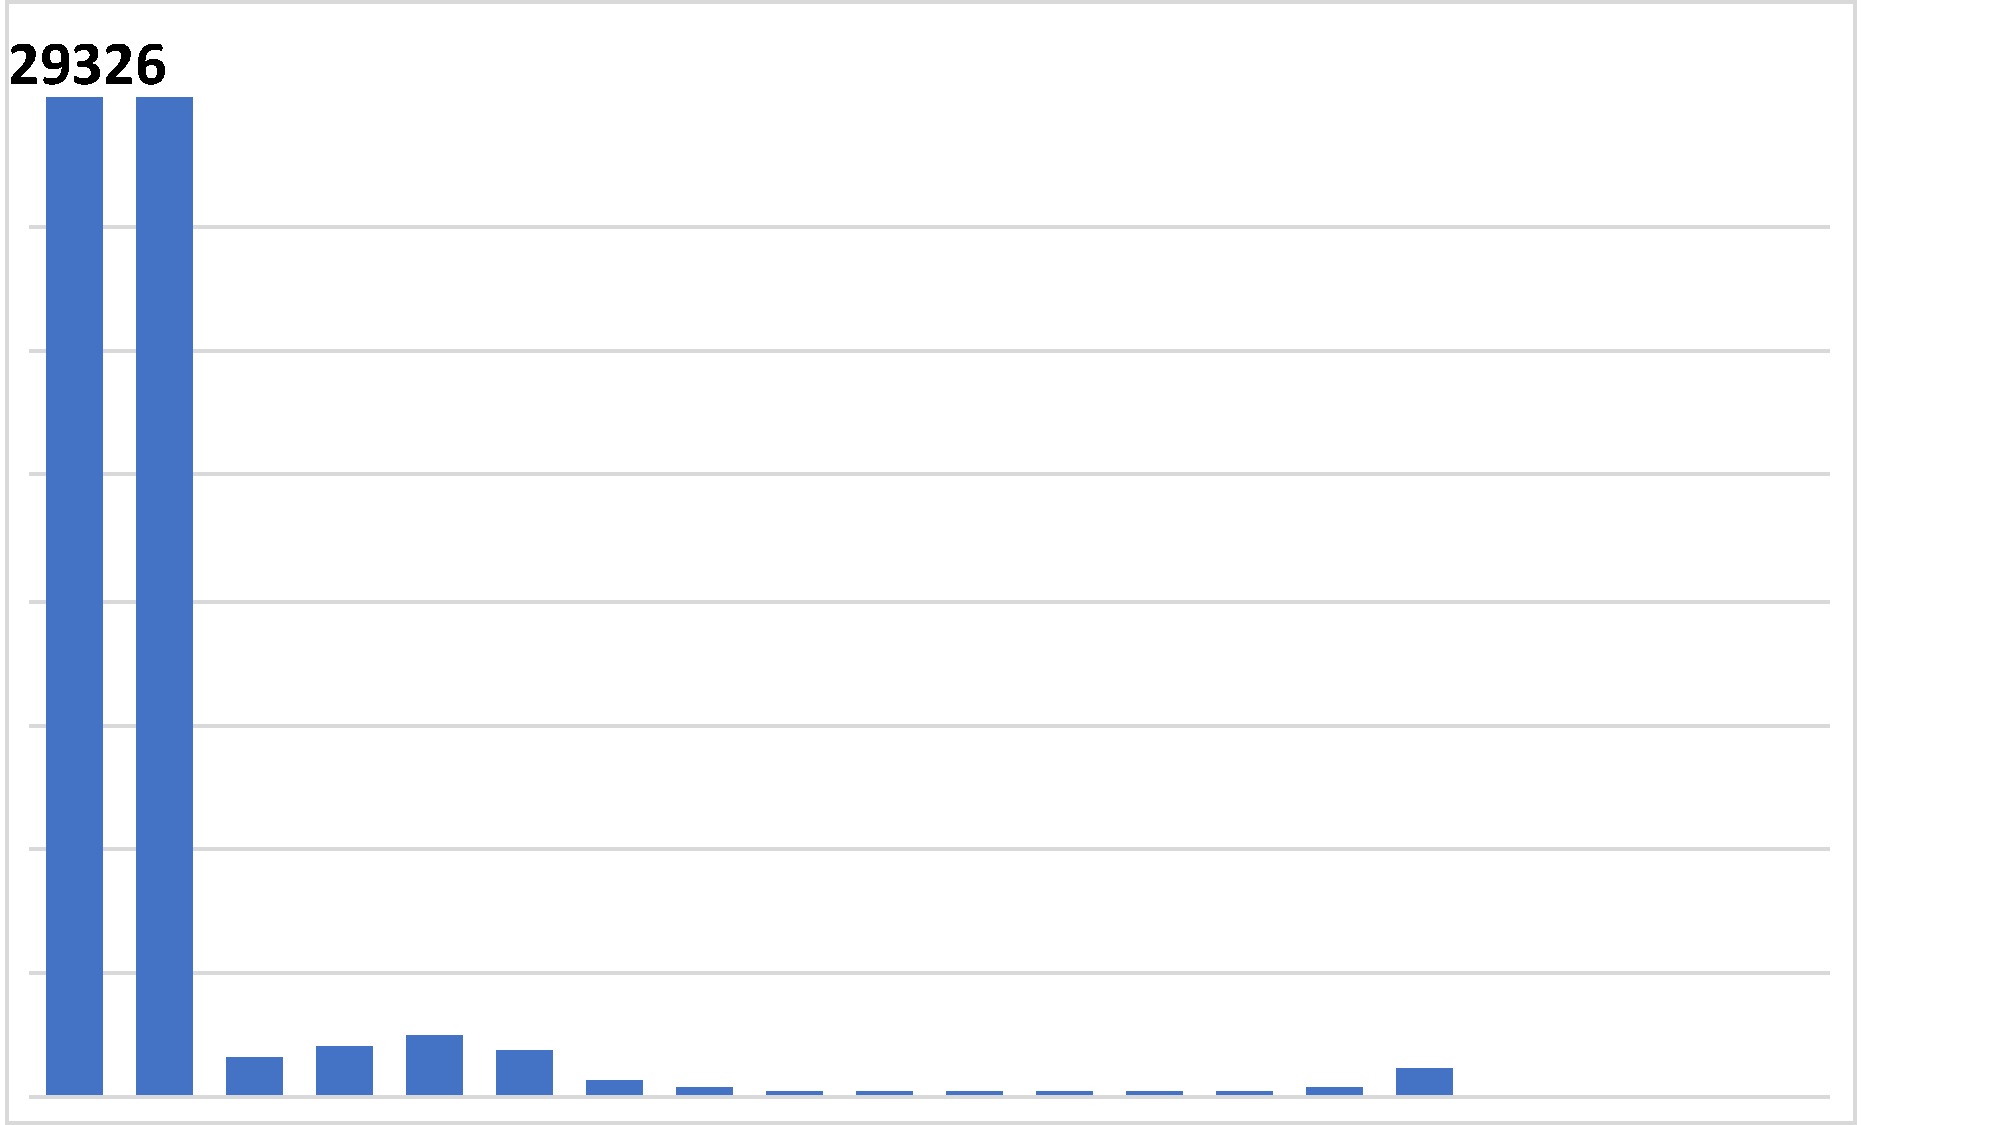
\includegraphics[width=0.95\linewidth, trim={0cm 0cm 2.5cm 0cm}, clip]{results/nyx/Eul50_AvgL2.pdf}
\vspace{-2mm}
\captionof{subfigure}{Eul 50 Avg$_{L2}$}
\end{minipage}
\begin{minipage}[t]{0.24\textwidth}%
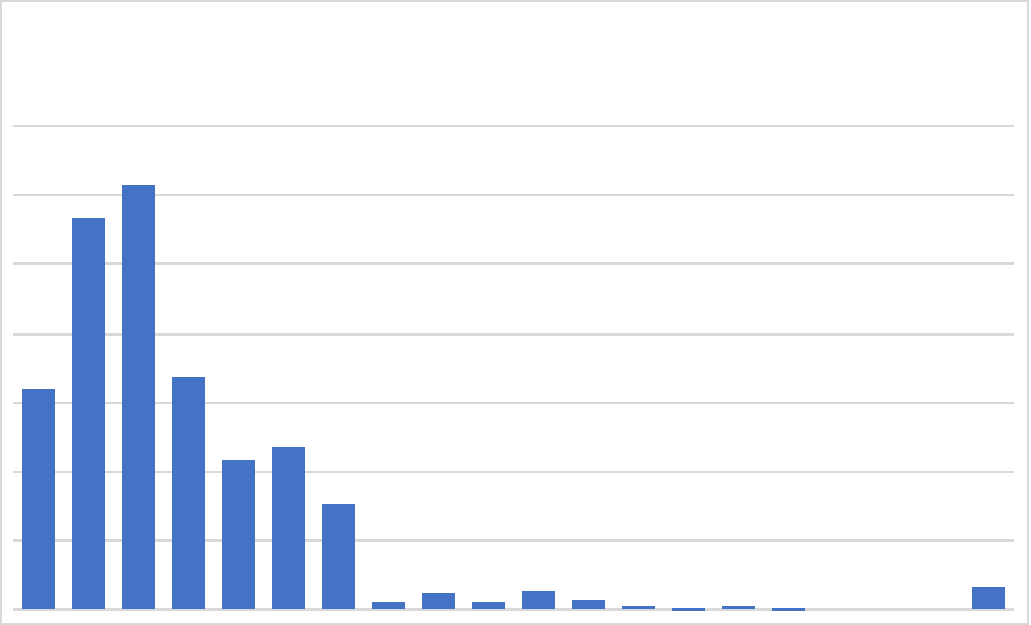
\includegraphics[width=0.95\linewidth]{results/nyx/Eul100_AvgL2.pdf}
\vspace{-2mm}
\captionof{subfigure}{Eul 100 Avg$_{L2}$}
\end{minipage}%
\hfill
\begin{minipage}[t]{0.24\textwidth}%
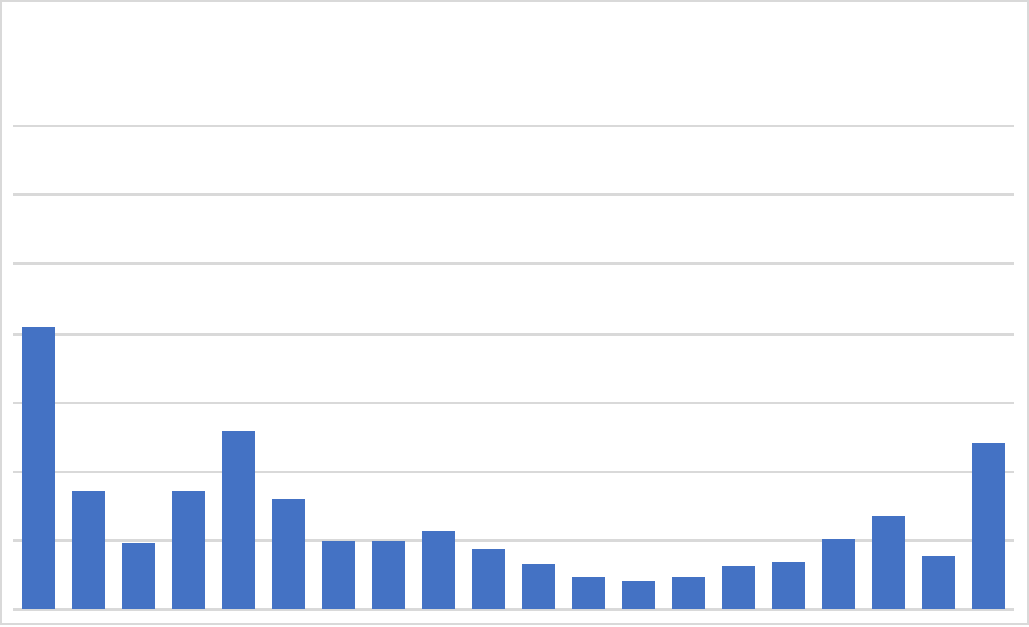
\includegraphics[width=0.95\linewidth]{results/nyx/Eul200_AvgL2.pdf}
\vspace{-2mm}
\captionof{subfigure}{Eul 200 Avg$_{L2}$}
\end{minipage}
\begin{minipage}[t]{0.24\textwidth}%
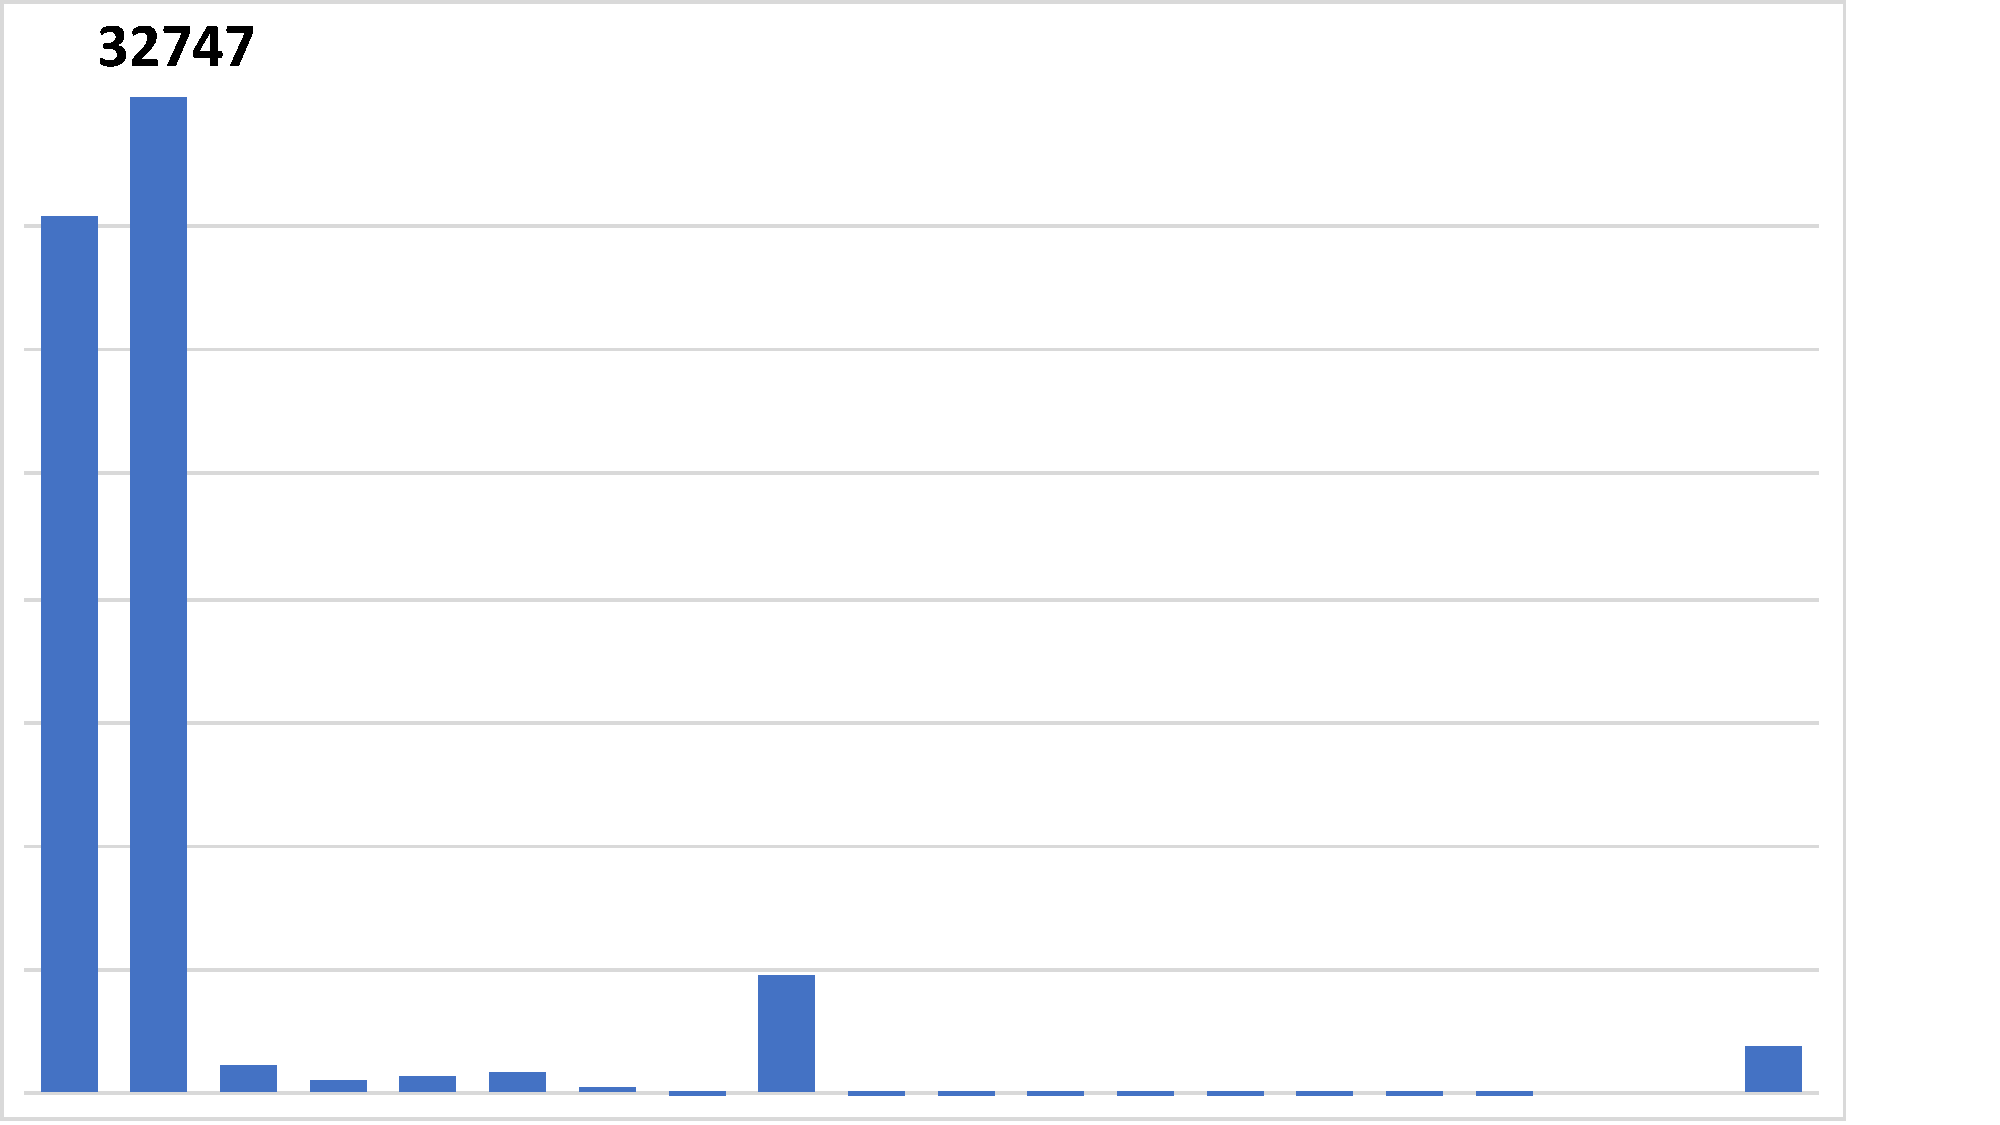
\includegraphics[width=0.95\linewidth, trim={0cm 0cm 2.5cm 0cm}, clip]{results/nyx/Eul25_Max.pdf}
\vspace{-2mm}
\captionof{subfigure}{Eul 25 Max$_{L2}$}
\end{minipage}%
\hfill
\begin{minipage}[t]{0.24\textwidth}%
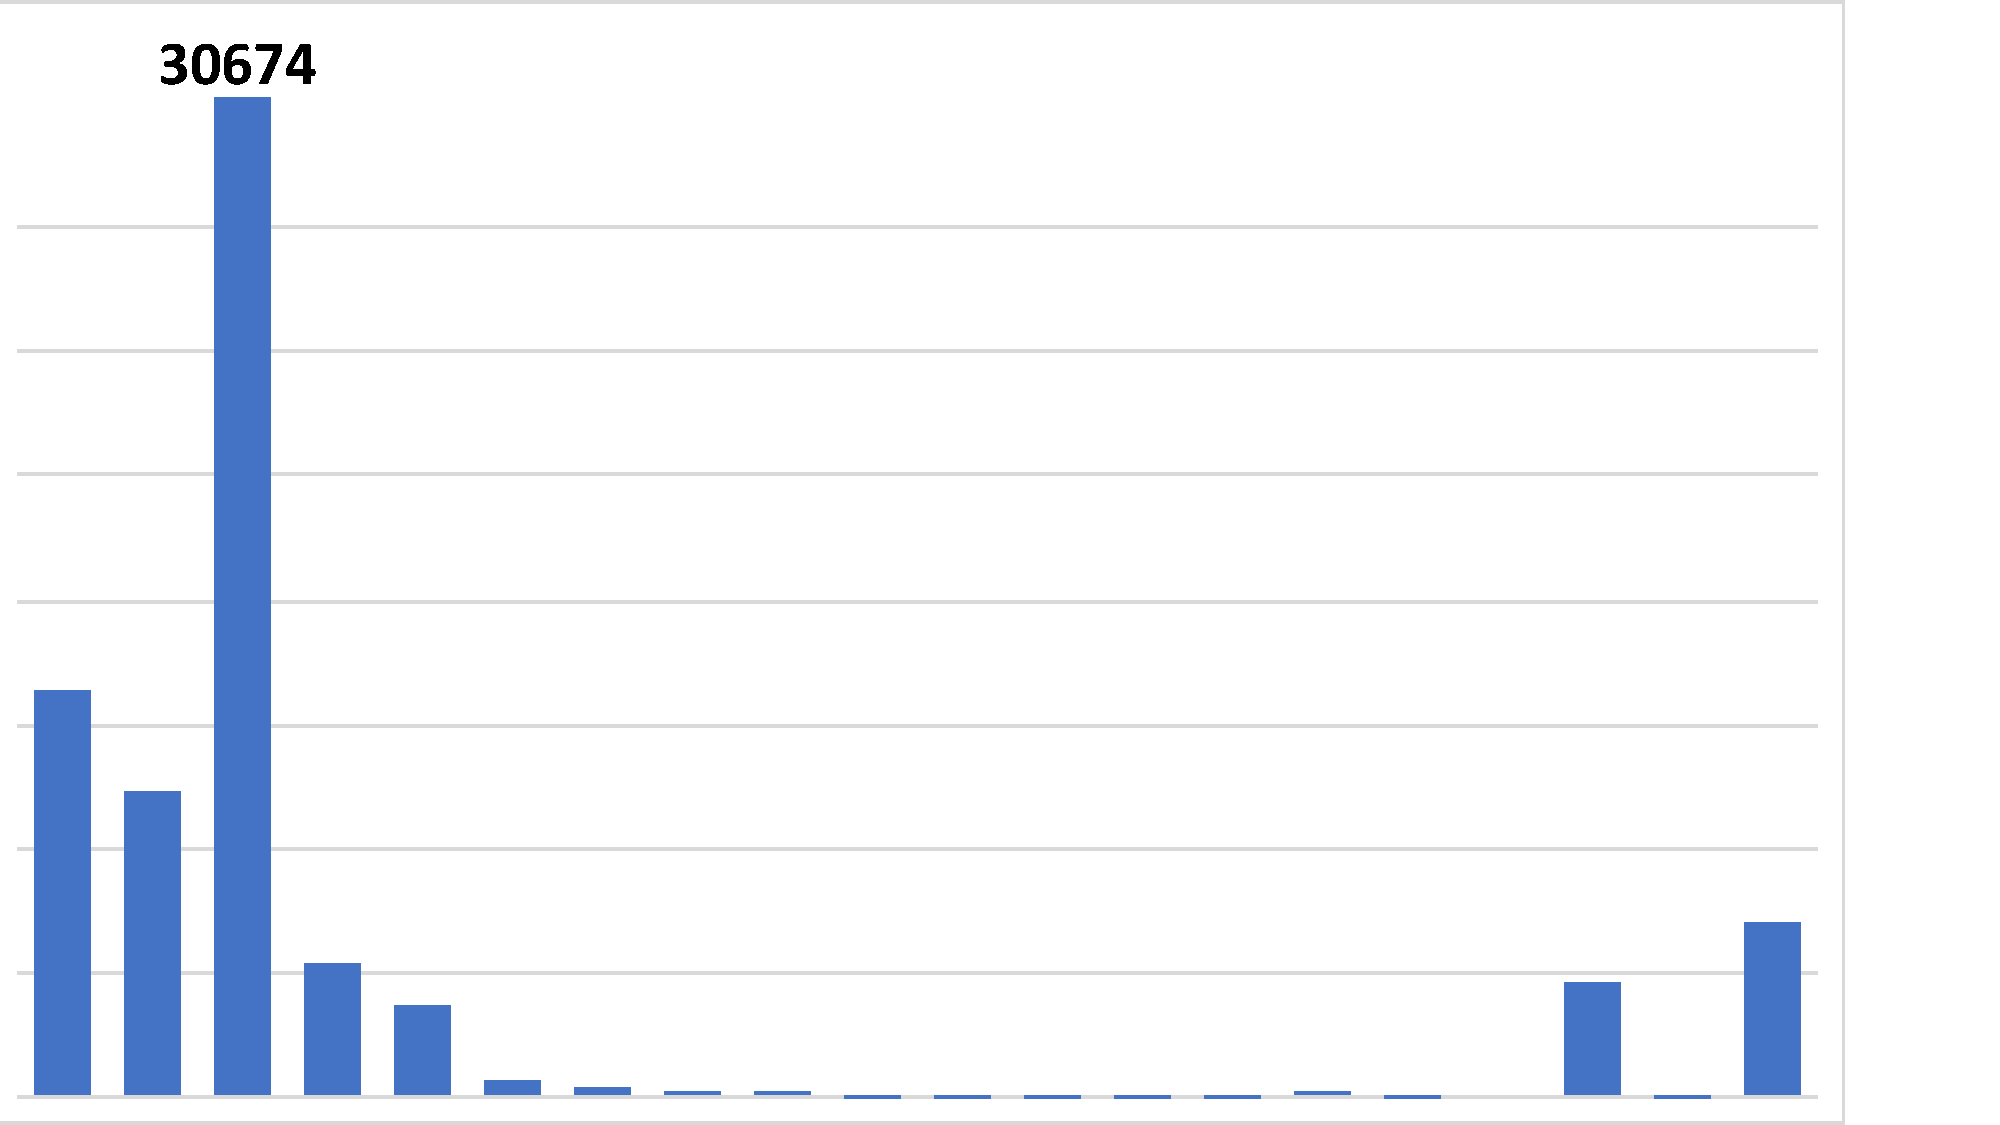
\includegraphics[width=0.95\linewidth, trim={0cm 0cm 2.5cm 0cm}, clip]{results/nyx/Eul50_Max.pdf}
\vspace{-2mm}
\captionof{subfigure}{Eul 50 Max$_{L2}$}
\end{minipage}
\begin{minipage}[t]{0.24\textwidth}%
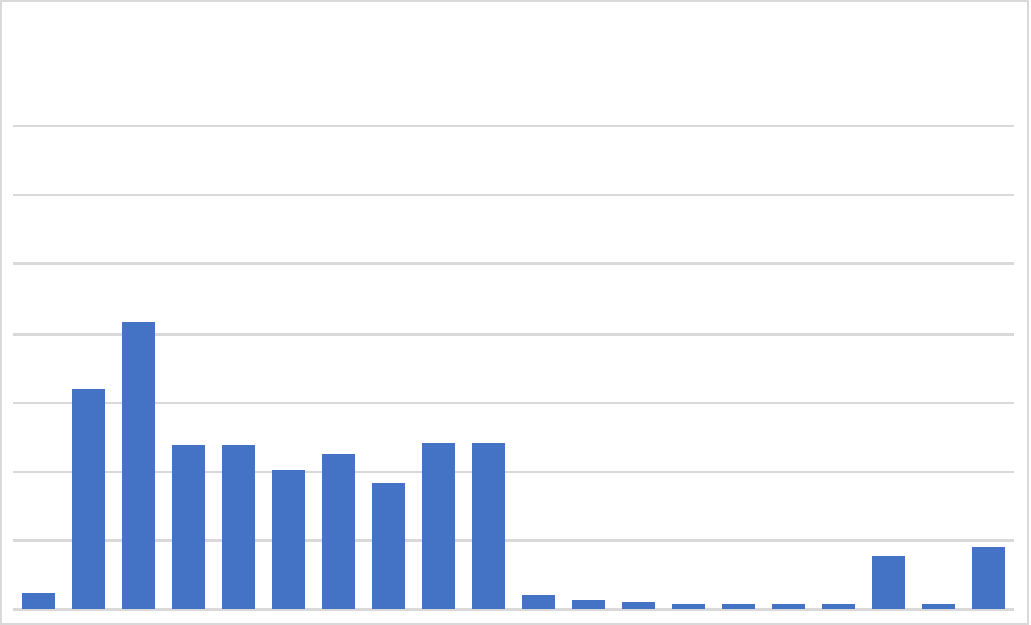
\includegraphics[width=0.95\linewidth]{results/nyx/Eul100_Max.pdf}
\vspace{-2mm}
\captionof{subfigure}{Eul 100 Max$_{L2}$}
\end{minipage}%
\hfill
\begin{minipage}[t]{0.24\textwidth}%
\includegraphics[width=0.95\linewidth]{results/nyx/Eul200_Max.pdf}
\vspace{-2mm}
\captionof{subfigure}{Eul 200 Max$_{L2}$}
\end{minipage}
%%%% Begin Nyx Lagrangian %%% 
\begin{minipage}[t]{0.24\textwidth}%
\includegraphics[width=0.95\linewidth, trim={0cm 0cm 2.5cm 0cm}, clip]{results/nyx/Lag25_1_AvgL2.pdf}
\vspace{-2mm}
\captionof{subfigure}{Lag 25 Avg$_{L2}$}
\end{minipage}%
\hfill
\begin{minipage}[t]{0.24\textwidth}%
\includegraphics[width=0.95\linewidth, trim={0cm 0cm 2.5cm 0cm}, clip]{results/nyx/Lag50_1_AvgL2.pdf}
\vspace{-2mm}
\captionof{subfigure}{Lag 50 Avg$_{L2}$}
\end{minipage}
\begin{minipage}[t]{0.24\textwidth}%
\includegraphics[width=0.95\linewidth, trim={0cm 0cm 2.5cm 0cm}, clip]{results/nyx/Lag100_1_AvgL2.pdf}
\vspace{-2mm}
\captionof{subfigure}{Lag 100 Avg$_{L2}$}
\end{minipage}%
\hfill
\begin{minipage}[t]{0.24\textwidth}%
\includegraphics[width=0.95\linewidth, trim={0cm 0cm 2.5cm 0cm}, clip]{results/nyx/Lag200_1_AvgL2.pdf}
\vspace{-2mm}
\captionof{subfigure}{Lag 200 Avg$_{L2}$}
\end{minipage}
\begin{minipage}[t]{0.24\textwidth}%
\includegraphics[width=0.95\linewidth, trim={0cm 0cm 2.5cm 0cm}, clip]{results/nyx/Lag25_1_Max.pdf}
\vspace{-2mm}
\captionof{subfigure}{Lag 25 Max$_{L2}$}
\end{minipage}%
\hfill
\begin{minipage}[t]{0.24\textwidth}%
\includegraphics[width=0.95\linewidth, trim={0cm 0cm 2.5cm 0cm}, clip]{results/nyx/Lag50_1_Max.pdf}
\vspace{-2mm}
\captionof{subfigure}{Lag 50 Max$_{L2}$}
\end{minipage}
\begin{minipage}[t]{0.24\textwidth}%
\includegraphics[width=0.95\linewidth, trim={0cm 0cm 2.5cm 0cm}, clip]{results/nyx/Lag100_1_Max.pdf}
\vspace{-2mm}
\captionof{subfigure}{Lag 100 Max$_{L2}$}
\end{minipage}%
\hfill
\begin{minipage}[t]{0.24\textwidth}%
\includegraphics[width=0.95\linewidth, trim={0cm 0cm 2.5cm 0cm}, clip]{results/nyx/Lag200_1_Max.pdf}
\vspace{-2mm}
\captionof{subfigure}{Lag 200 Max$_{L2}$}
\end{minipage}
\end{framed}
\vspace{-2mm}
\captionof{figure}{\textbf{Nyx} experiment histograms for 50,000 test particle interpolation errors. Each plot has 20 bins, ranging from 0 to $>$0.44, with bar height encoding number of particles. Horizontal grid lines mark increments of 2,000.}
\label{fig:nyx_histograms}
\end{minipage}%
\vspace{-6mm}
\end{figure*}


\subsection{Post Hoc Efficacy}
\label{sec:results_posthoc}
\begingroup
\setlength{\tabcolsep}{0pt}
%\renewcommand{\arraystretch}{0.55} % Default value: 1
%\setlength{\fboxsep}{1mm}
\begin{table*}[t]
\centering
\begin{tabular}{|P{2cm}|P{1.3cm}|P{2cm}|L{1.3cm} P{1.7cm} D |P{8cm}|}
\hline
Technique & Interval & Reduction & Data & AvgN$_{L2}$ & Cell  & \multirow{2}{*}{Scatter Plot} \\
& & & & & Side\% & \\
\hline
\multicolumn{6}{l}{\textbf{          Cloverleaf3D Proxy Hydrodynamics Application }} & \multirow{12}{*}{\includegraphics[width=0.95\linewidth]{images/cloverleaf_accuracy.pdf}}\\
\cline{1-6}
\multirow{3}{*}{Eulerian} & 20 & \multirow{3}{*}{Full Res} & 267 GB & 0.0197 & 116.17 &  \\
\cline{2-2}
& 40 & & 133 GB & 0.0459 & 270.49 & \\
\cline{2-2}
& 60 & & 95 GB & 0.0725 & 426.96 &  \\
\cline{1-6}
\multirow{9}{*}{Lagrangian} & \multirow{3}{*}{20} & 1:8 & 34 GB & 0.0032 & 18.928 & \\
\cline{3-3}
 & & 1:27 & 10 GB & 0.0040 & 23.891 & \\
\cline{3-3}
 & & 1:64 & 4 GB & 0.0040 & 23.583 & \\
\cline{2-3}
& \multirow{3}{*}{40} & 1:8 & 17 GB & 0.0043 & 25.646 &  \\
\cline{3-3}
& & 1:27 & 5.1 GB & 0.0049 & 29.145 &  \\
\cline{3-3}
& & 1:64 & 2 GB & 0.0053 & 31.353 & \\
\cline{2-3}
& \multirow{3}{*}{60} & 1:8 & 12 GB & 0.0064 & 37.882 & \\
\cline{3-3}
& & 1:27 & 3.4 GB & 0.0066 & 39.002 & \multirow{6}{*}{\raisebox{-33.5mm}[0pt][0pt]{\includegraphics[width=0.95\linewidth]{images/sw4_accuracy.pdf}}} \\
\cline{3-3}
& & 1:64 & 1.3 GB & 0.0070 & 41.247 & \\
\cline{1-6}
\multicolumn{6}{l}{\textbf{          SW4 Seismic Wave Modeling Simulation }} &  \\
\cline{1-6}
\multirow{2}{*}{Eulerian} & 250 & \multirow{2}{*}{Full Res} & 1100 MB & 3.5714 & 0.9224 & \\
\cline{2-2}
 & 500 & & 550 MB & 5.0493 & 1.3023  & \\
\cline{1-6}
\multirow{4}{*}{Lagrangian} & \multirow{4}{*}{250} & 1:1 & 1300 MB & 0.0005 & 0.0001  &  \\
\cline{3-3}
 &  & 1:8 & 158 MB & 0.0033 & 0.0008 &  \\
\cline{3-3}
 &  & 1:27 & 42 MB & 0.0072 & 0.0018 & \\
\cline{3-3}
 &  & 1:64 & 16 MB & 0.0128 & 0.0031 &  \\
\cline{1-6}
\multicolumn{6}{l}{\textbf{          Nyx Cosmology Simulation }} & \\
\cline{1-6}
\multirow{4}{*}{Eulerian} & 25 & \multirow{4}{*}{Full Res} & 227 MB & 0.010 & 2.2954 &  \\
\cline{2-2}%\cline{4-6}
& 50 & & 120 MB & 0.037 & 8.4090 &  \multirow{16}{*}{\includegraphics[width=0.95\linewidth]{images/nyx_accuracy.pdf}}\\
\cline{2-2}%\cline{4-6}
& 100 & & 67 MB & 0.090 & 20.454 & \\
\cline{2-2}%\cline{4-6}
& 200 & & 40 MB & 0.265 & 60.227 & \\
\cline{1-6}
\multirow{12}{*}{Lagrangian} & \multirow{3}{*}{25} & 1:1 & 232 MB & 0.051 & 11.613 & \\
\cline{3-3}
& & 1:8 & 27 MB & 0.164 & 37.272 &  \\
\cline{3-3}
& & 1:27 & 8 MB & 0.320 & 72.727 &  \\
\cline{2-3}
& \multirow{3}{*}{50} & 1:1 & 166 MB & 0.059 & 13.409 & \\
\cline{3-3}
& & 1:8 & 14 MB & 0.153 & 34.772 &  \\
\cline{3-3}
& & 1:27 & 4 MB & 0.256 & 58.181 &  \\
\cline{2-3}
& \multirow{3}{*}{100} & 1:1 & 58 MB & 0.067 & 15.227 &  \\
\cline{3-3}
& & 1:8 & 7 MB & 0.159 & 36.136 &  \\
\cline{3-3}
& & 1:27 & 2 MB & 0.261 & 59.318 & \\
\cline{2-3}
 & \multirow{3}{*}{200} & 1:1 & 29 MB & 0.103 & 23.409 &  \\
\cline{3-3}
& & 1:8 & 3.4 MB & 0.204 & 46.363 & \\
\cline{3-3}
& & 1:27 & 1 MB & 0.321 & 72.954 &  \\
\hline
\end{tabular}
\vspace{-3mm}
\caption{\textit{Post hoc} efficacy evaluation and experiment configurations for our three simulation codes.}
\label{table:accuracy}
\vspace{-5mm}
\end{table*}
\endgroup

\begin{figure*}
\begin{subfigure}{0.195\textwidth}
\centering
\includegraphics[width=0.9\linewidth]{results/cloverleaf3d/eul_1/Eul1_AvgL2.pdf}
\vspace{-2mm}
\caption{Eul 20 Avg$_{L2}$ L2 }
\end{subfigure}
\begin{subfigure}{0.195\textwidth}
\centering
\includegraphics[width=0.95\linewidth]{results/cloverleaf3d/eul_2/Eul2_AvgL2.pdf}
\vspace{-2mm}
\caption{Eul 40 Avg$_{L2}$ L2 }
\end{subfigure}
\begin{subfigure}{0.195\textwidth}
\centering
\includegraphics[width=0.9\linewidth, trim={0cm 0cm 2.5cm 0cm}, clip]{results/cloverleaf3d/lag_4/Lag4_AvgL2.pdf}
\vspace{-2mm}
\caption{Lag 40 1:8 Avg$_{L2}$ }
\end{subfigure}
\begin{subfigure}{0.195\textwidth}
\centering
\includegraphics[width=0.9\linewidth, trim={0cm 0cm 2.5cm 0cm}, clip]{results/cloverleaf3d/lag_5/Lag5_AvgL2.pdf}
\vspace{-2mm}
\caption{Lag 40 1:27 Avg$_{L2}$ }
\end{subfigure}
\begin{subfigure}{0.195\textwidth}
\centering
\includegraphics[width=0.9\linewidth, trim={0cm 0cm 2.5cm 0cm}, clip]{results/cloverleaf3d/lag_6/Lag6_AvgL2.pdf}
\vspace{-2mm}
\caption{Lag 40 1:64 Avg$_{L2}$ }
\end{subfigure}
\begin{subfigure}{0.195\textwidth}
\centering
\includegraphics[width=0.9\linewidth]{results/cloverleaf3d/eul_1/Eul1_Max.pdf}
\vspace{-2mm}
\caption{Eul 20 Max$_{L2}$ }
\end{subfigure}
\begin{subfigure}{0.195\textwidth}
\centering
\includegraphics[width=0.95\linewidth]{results/cloverleaf3d/eul_2/Eul2_Max.pdf}
\vspace{-2mm}
\caption{Eul 40 Max$_{L2}$ }
\end{subfigure}
\hspace{0.2mm}
\begin{subfigure}{0.195\textwidth}
\centering
\includegraphics[width=0.9\linewidth, trim={0cm 0cm 2.5cm 0cm}, clip]{results/cloverleaf3d/lag_4/Lag4_Max.pdf}
\vspace{-2mm}
\caption{Lag 40 1:8 Max$_{L2}$ }
\end{subfigure}
\begin{subfigure}{0.195\textwidth}
\centering
\includegraphics[width=0.9\linewidth, trim={0cm 0cm 2.5cm 0cm}, clip]{results/cloverleaf3d/lag_5/Lag5_Max.pdf}
\vspace{-2mm}
\caption{Lag 40 1:27 Max$_{L2}$}
\end{subfigure}
\begin{subfigure}{0.195\textwidth}
\centering
\includegraphics[width=0.9\linewidth, trim={0cm 0cm 2.5cm 0cm}, clip]{results/cloverleaf3d/lag_6/Lag6_Max.pdf}
\vspace{-2mm}
\caption{Lag 40 1:64 Max$_{L2}$}
\end{subfigure}
%\begin{subfigure}{0.24\textwidth}
%\includegraphics[width=0.9\linewidth]{results/cloverleaf3d/eul_1/Eul1_EndPt.pdf}
%\caption{Eulerian 20 End Point}
%\end{subfigure}
%\hspace{1mm}
%\begin{subfigure}{0.21\textwidth}
%\includegraphics[width=1\linewidth]{results/cloverleaf3d/lag_4/Lag4_EndPt.pdf}
%\caption{Lagrangian 40 1:8 End Point}
%\end{subfigure}
%\hspace{1mm}
%\begin{subfigure}{0.21\textwidth}
%\includegraphics[width=1\linewidth]{results/cloverleaf3d/lag_5/Lag5_EndPt.pdf}
%\caption{Lagrangian 40 1:27 End Point}
%\end{subfigure}
%\hspace{1mm}
%\begin{subfigure}{0.21\textwidth}
%\includegraphics[width=1\linewidth]{results/cloverleaf3d/lag_6/Lag6_EndPt.pdf}
%\caption{Lagrangian 40 1:64 End Point}
%\end{subfigure}
\vspace{-3mm}
\caption{\textbf{Cloverleaf3D} experiment histograms for 100,000 test particle interpolation errors. Each plot has 25 bins, ranging from 0 to $>$0.05, with bar height encoding number of particles. Horizontal grid lines mark increments of 5,000.} 
\label{fig:clover_histograms}
\vspace{-6mm}
\end{figure*}


Table~\ref{table:accuracy} contains the results of our experiments for this campaign using all three simulation codes.
%
For each simulation code we consider multiple options of number of particles and interval.
%
Varying either of these parameters impacts \textbf{PHE-1}, \textbf{PHE-2}, and \textbf{DS-1}.
%
The \textbf{Cell Side\%} column in Table~\ref{table:accuracy} redundantly encodes the value in each cell using cell background color (white to pure red hue for the range [0,100], where 0 or white indicates a particle is perfectly accurate and 100+ or pure red indicates particles on average are at least a grid cell side away from ground truth).
%
In addition to Table~\ref{table:accuracy}, our empirical study includes a more detailed look at per particle interpolation error using histograms.
%
We present a set of histograms for each simulation code. 
%
For each histogram chart we exclude the axes and instead describe the common details of the plot in the captions (number of bins, range, horizontal grid line increment, etc.) and use annotation to mark histogram bars whose height exceeds the plot area.
%
Although use of an annotation rather than the true height of the bar visually misrepresents a single data point in some plots, we believe this tradeoff is worth the closer look at the remaining data points.


%We separate our discussion of post hoc efficacy based on \textbf{PHE-1} and \textbf{PHE-2}.
%
%Our quantitative evaluation of accuracy is in Section~\ref{sec:accuracy} and post hoc distributed-memory interpolation costs are reported in Section~\ref{sec:posthoc_costs}. 
\subsubsection{Cloverleaf3D Hydrodynamics Proxy Simulation}
For the Cloverleaf3D time-dependent vector field, we considered 3 options for both number of particles and interval, to encode the behavior of the field.
%
We randomly placed 100,000 test particles in the domain and tested the accuracy of reconstructed trajectories.
%
We use the first 600 cycles of the simulation and set step size to 0.0045.
%
Overall, we observed that the Lagrangian technique performed significantly better and offered improved data storage-accuracy propositions.

With respect to \textbf{DS-1} and \textbf{PHE-1}, even a 100X data reduction results in improved accuracy compared to storing a full resolution Eulerian grid more frequently. 
%
For example, a Lagrangian configuration using 1:64 number of particles and an interval of 60 stores 1.3 GB over 600 cycles, and has an \textbf{AvgN$_{L2}$} of 41.2\% of the cell side. 
%
In comparison, an Eulerian configuration storing the full mesh every 40 cycles requires 133 GB over 600 cycles, and has an \textbf{AvgN$_{L2}$} of 270.4\% of the cell side.
%
For all the Lagrangian configurations, the \textbf{AvgN$_{L2}$} was low and particles on average remained within the same cell as the ground truth.
%

Although this proxy simulation demonstrates very clearly the shortcomings of the Eulerian technique as the interval increases, we observed that the Lagrangian technique benefits minimally from an increase in the number of particles.
%
We believe this is due to Cloverleaf3D being a miniapp, where increasing the spatial resolution does not increase the complexity of the physics, i.e., no new features are introduced as they would be in a real-world simulation.
%
That being said, even if the Eulerian technique used multi-resolution to achieve reduced storage, it would be less accurate than Lagrangian, given using the full spatial resolution is less accurate. 

The histogram plots in Figure~\ref{fig:clover_histograms} show the distribution of particle interpolation error clearly indicating the superiority of the Lagrangian technique for \textbf{EUS}.
%
Comparing the histogram plots, although Eulerian (267 GB) is storing full resolution data sets twice as often, the number of test particles with a \textbf{Max$_{L2}$} of over 300\% of the cell side distance (right-end bin in each plot) is over 15\%, compared to less than 5\% for Lagrangian (2 GB to 17 GB) in all cases.
%
This provides intuition regarding the ``rate of inaccurate interpolation'' for each technique for the \textbf{EUS} problem.

\begingroup
\begin{table}[!h]
\centering
\scalebox{0.9}{
\begin{tabular}{|c|c|c|c|}
\hline
Samples & CGAL & Interpolation & Communication \\
/Rank & Delaunay (s) & (s) & (s) \\
\hline
7.2M & 178 & 0.00246 & \multirow{3}{*}{0.00125} \\
2.1M & 53 & 0.00141 & \\
887k & 21 & 0.00093 & \\
\hline
\end{tabular}
}
\vspace{-3mm}
\caption{Distributed memory \textit{post hoc} interpolation cost for 100,000 particles across a \textbf{single interval} of the Cloverleaf3D extracted data using 16 compute nodes and 96 MPI ranks on Summit. Values averaged over all reconstruction runs.}
\label{table:reconstruction}
\end{table}
\endgroup


For \textbf{PHE-2}, we measured the time required for Cloverleaf3D reconstructions.
%
In our empirical study, we only reconstructed Cloverleaf3D pathlines in a distributed-memory setting (16 nodes, 96 MPI ranks).
%
Table~\ref{table:reconstruction} contains timings for our reconstruction method for a single interval given a workload, i.e., number of samples to be triangulated and interpolated per rank.
%
%The total reconstruction cost \textbf{PHE-2} of entire pathlines depends on the number of intervals spanning the total number of cycles.
%
%Although shorter intervals offers higher resolution in terms of number of known interpolated points along a reconstructed pathline, longer intervals offers less total reconstruction time.
%
The most dominant cost during this process is the search structure construction, i.e., the Delaunay triangulation.
%
Although we avoid the prohibitive cost of a global Delaunay triangulation with our implementation, we believe there is room for improvement.
%
That being said, for reduced Lagrangian representations, the parallel Delaunay construction cost can be low compared to the Eulerian approach that requires performing interpolation and communication for every cycle.
%
For example, the Lagrangian configuration using an interval of 40 and 1:27 number of particles, can be used to construct pathlines for 100,000 particles across 600 cycles in under 6 minutes (excluding I/O).
%
For an Eulerian approach to be faster, it would need to compute each cycle in 0.6 seconds (our implementation required 0.47 seconds per cycle excluding I/O).



\subsubsection{SW4 Seismic Wave Propagation Simulation}
For the SW4 simulation, we considered 4 options for number of particles.
%
%The SW4 simulation is great example of a situation where the Lagrangian approach is better able to encode time-dependent vector field behavior.
%
The SW4 simulation generates a displacement vector field that captures the wave propagation modeled in the simulation. 
%
In this case, the Lagrangian representation is far better equipped than the traditional method to accurately encode this transient behavior in the domain. 
%
Our experiments considered 2000 cycles of the simulation, and evaluated accuracy by reconstructing 90,000 test particle trajectories placed randomly between Z=5,000 and Z=15,000 (the layer of most activity in the domain) using a step size of 1.

The SW4 simulation domain extents are very large, thus each cell side is approximately 387 in our experiments.
%
The \textbf{AvgN$_{L2}$} value of our test particles indicates all particles remained within the cell, with the Lagrangian technique offering near perfect reconstruction, while the Eulerian technique only suffers from an error of 1\% of the cell side by this measure.
%
However, displacement values in an earthquake simulation are expected to be small and an error of even that magnitude might represent failure to capture the wave propagation.
%

The SW4 histogram plots (Figure~\ref{fig:sw4_histograms}) use different bin ranges for Lagrangian and Eulerian given the distributions were very different.
%
The plots show the an increase in error for the Eulerian technique as the interval increases and an increase in error for the Lagrangian technique as the number of particles used decreases from 1:27 to 1:64.
%

Overall, the Lagrangian technique offers excellent propositions for \textbf{DS-1} and \textbf{PHE-1}.
%
The Lagrangian technique was able to preserve near perfect integrity with upto 70X less data storage.
\subsubsection{Nyx Cosmology Simulation}
For the Nyx cosmology simulation, we considered 4 options for number of particles and interval to provide an understanding across a wider spatiotemporal range.
%
Figure~\ref{fig:vectorfield_nyx} shows a slice of the Nyx vector field at two three slices~(0, 200, 400).
%
We observed that the unit vectors at each grid point in the domain remain relatively the same across all cycles.
%
The slow evolution of the vector field is in terms of velocity magnitude in few regions of the domain.
%
The maximum velocity magnitude in the domain increases steadily for the 400 cycles of the simulation we use in this study.
%
Our experiments considered 50,000 test particle trajectories placed randomly in the domain and set a step size to 0.02.
\begin{figure}[h]
\centering
\includegraphics[width=1\linewidth, trim={0cm 1.1cm 0cm 0cm}, clip]{images/Nyx_vectorfields.pdf}
\vspace{-5mm}
\caption{Nyx vector field visualization: (a) and (d) show the vector field at time 0 and the maximum velocity magnitude is 52.02, (b) and (e) show the vector field at time 200 and the maximum velocity magnitude is 145.0, and finally, (c) and (f) show the vector field at time 400 and the maximum velocity is 571.2.}
\label{fig:vectorfield_nyx}
\vspace{-3mm}
\end{figure}




\begin{figure*}
\begin{minipage}[t]{0.33\linewidth}%
\begin{framed}
\setcounter{subfigure}{0}
\begin{minipage}[t]{0.49\textwidth}%
\centering
\includegraphics[width=0.95\textwidth]{results/sw4/Eul1_AvgL2.pdf}%
\vspace{-3mm}
\captionof{subfigure}{\footnotesize{Eul 250 Avg$_{L2}$}}
\end{minipage}%
\hfill
\begin{minipage}[t]{0.49\textwidth}%
\centering
\includegraphics[width=0.95\linewidth]{results/sw4/Eul2_AvgL2.pdf}
\vspace{-3mm}
\captionof{subfigure}{\footnotesize{Eul 500 Avg$_{L2}$}} 
\end{minipage}
\begin{minipage}[t]{0.49\textwidth}%
\centering
\includegraphics[width=0.95\textwidth]{results/sw4/Eul1_Max.pdf}%
\vspace{-3mm}
\captionof{subfigure}{\footnotesize{Eul 250 Max$_{L2}$}}
\end{minipage}%
\hfill
\begin{minipage}[t]{0.49\textwidth}%
\centering
\includegraphics[width=0.95\linewidth]{results/sw4/Eul2_Max.pdf}
\vspace{-3mm}
\captionof{subfigure}{\footnotesize{Eul 500 Max$_{L2}$}} 
\end{minipage}
\begin{minipage}[t]{0.49\textwidth}%
\centering
\includegraphics[width=0.95\linewidth, trim={0cm 0cm 2.5cm 0cm}, clip]{results/sw4/Lag3_AvgL2.pdf}
\vspace{-3mm}
\captionof{subfigure}{\footnotesize{Lag 250 1:27 Avg$_{L2}$}}
\end{minipage}%
\hfill
\begin{minipage}[t]{0.49\textwidth}%
\centering
\includegraphics[width=0.95\linewidth, trim={0cm 0cm 2.5cm 0cm}, clip]{results/sw4/Lag4_AvgL2.pdf}
\vspace{-3mm}
\captionof{subfigure}{\footnotesize{Lag 250 1:64 Avg$_{L2}$}} 
\end{minipage}
\begin{minipage}[t]{0.49\textwidth}%
\centering
\includegraphics[width=0.95\linewidth, trim={0cm 0cm 2.5cm 0cm}, clip]{results/sw4/Lag3_Max.pdf}
\vspace{-3mm}
\captionof{subfigure}{\footnotesize{Lag 250 1:27 Max$_{L2}$}}
\end{minipage}%
\hfill
\begin{minipage}[t]{0.49\textwidth}%
\centering
\includegraphics[width=0.95\linewidth, trim={0cm 0cm 2.5cm 0cm}, clip]{results/sw4/Lag4_Max.pdf}
\vspace{-3mm}
\captionof{subfigure}{\footnotesize{Lag 250 1:64 Max$_{L2}$}} 
\end{minipage}
\end{framed}
\vspace{-2mm}
\captionof{figure}{\textbf{SW4} experiment histograms for 90,000 test particle interpolation errors. Each plot has 25 bins, Eulerian bins range from $<$0.6 to $>$15, Lagrangian bins range from 0 to $>$0.2, with bar height encoding number of particles. Horizontal grid lines mark increments of 2,000.}
\label{fig:sw4_histograms}
\end{minipage}% End of SW4
%%%%%%%%%%%%%%%%%%%%%%%%%%%%%%%%%%%
\setcounter{subfigure}{0}
\hfill
\begin{minipage}[t]{0.66\linewidth}%
\begin{framed}
\begin{minipage}[t]{0.24\textwidth}%
\includegraphics[width=0.95\linewidth, trim={0cm 0cm 2.5cm 0cm}, clip]{results/nyx/Eul25_AvgL2.pdf}
\vspace{-2mm}
\captionof{subfigure}{Eul 25 Avg$_{L2}$}
\end{minipage}%
\hfill
\begin{minipage}[t]{0.24\textwidth}%
\includegraphics[width=0.95\linewidth, trim={0cm 0cm 2.5cm 0cm}, clip]{results/nyx/Eul50_AvgL2.pdf}
\vspace{-2mm}
\captionof{subfigure}{Eul 50 Avg$_{L2}$}
\end{minipage}
\begin{minipage}[t]{0.24\textwidth}%
\includegraphics[width=0.95\linewidth]{results/nyx/Eul100_AvgL2.pdf}
\vspace{-2mm}
\captionof{subfigure}{Eul 100 Avg$_{L2}$}
\end{minipage}%
\hfill
\begin{minipage}[t]{0.24\textwidth}%
\includegraphics[width=0.95\linewidth]{results/nyx/Eul200_AvgL2.pdf}
\vspace{-2mm}
\captionof{subfigure}{Eul 200 Avg$_{L2}$}
\end{minipage}
\begin{minipage}[t]{0.24\textwidth}%
\includegraphics[width=0.95\linewidth, trim={0cm 0cm 2.5cm 0cm}, clip]{results/nyx/Eul25_Max.pdf}
\vspace{-2mm}
\captionof{subfigure}{Eul 25 Max$_{L2}$}
\end{minipage}%
\hfill
\begin{minipage}[t]{0.24\textwidth}%
\includegraphics[width=0.95\linewidth, trim={0cm 0cm 2.5cm 0cm}, clip]{results/nyx/Eul50_Max.pdf}
\vspace{-2mm}
\captionof{subfigure}{Eul 50 Max$_{L2}$}
\end{minipage}
\begin{minipage}[t]{0.24\textwidth}%
\includegraphics[width=0.95\linewidth]{results/nyx/Eul100_Max.pdf}
\vspace{-2mm}
\captionof{subfigure}{Eul 100 Max$_{L2}$}
\end{minipage}%
\hfill
\begin{minipage}[t]{0.24\textwidth}%
\includegraphics[width=0.95\linewidth]{results/nyx/Eul200_Max.pdf}
\vspace{-2mm}
\captionof{subfigure}{Eul 200 Max$_{L2}$}
\end{minipage}
%%%% Begin Nyx Lagrangian %%% 
\begin{minipage}[t]{0.24\textwidth}%
\includegraphics[width=0.95\linewidth, trim={0cm 0cm 2.5cm 0cm}, clip]{results/nyx/Lag25_1_AvgL2.pdf}
\vspace{-2mm}
\captionof{subfigure}{Lag 25 Avg$_{L2}$}
\end{minipage}%
\hfill
\begin{minipage}[t]{0.24\textwidth}%
\includegraphics[width=0.95\linewidth, trim={0cm 0cm 2.5cm 0cm}, clip]{results/nyx/Lag50_1_AvgL2.pdf}
\vspace{-2mm}
\captionof{subfigure}{Lag 50 Avg$_{L2}$}
\end{minipage}
\begin{minipage}[t]{0.24\textwidth}%
\includegraphics[width=0.95\linewidth, trim={0cm 0cm 2.5cm 0cm}, clip]{results/nyx/Lag100_1_AvgL2.pdf}
\vspace{-2mm}
\captionof{subfigure}{Lag 100 Avg$_{L2}$}
\end{minipage}%
\hfill
\begin{minipage}[t]{0.24\textwidth}%
\includegraphics[width=0.95\linewidth, trim={0cm 0cm 2.5cm 0cm}, clip]{results/nyx/Lag200_1_AvgL2.pdf}
\vspace{-2mm}
\captionof{subfigure}{Lag 200 Avg$_{L2}$}
\end{minipage}
\begin{minipage}[t]{0.24\textwidth}%
\includegraphics[width=0.95\linewidth, trim={0cm 0cm 2.5cm 0cm}, clip]{results/nyx/Lag25_1_Max.pdf}
\vspace{-2mm}
\captionof{subfigure}{Lag 25 Max$_{L2}$}
\end{minipage}%
\hfill
\begin{minipage}[t]{0.24\textwidth}%
\includegraphics[width=0.95\linewidth, trim={0cm 0cm 2.5cm 0cm}, clip]{results/nyx/Lag50_1_Max.pdf}
\vspace{-2mm}
\captionof{subfigure}{Lag 50 Max$_{L2}$}
\end{minipage}
\begin{minipage}[t]{0.24\textwidth}%
\includegraphics[width=0.95\linewidth, trim={0cm 0cm 2.5cm 0cm}, clip]{results/nyx/Lag100_1_Max.pdf}
\vspace{-2mm}
\captionof{subfigure}{Lag 100 Max$_{L2}$}
\end{minipage}%
\hfill
\begin{minipage}[t]{0.24\textwidth}%
\includegraphics[width=0.95\linewidth, trim={0cm 0cm 2.5cm 0cm}, clip]{results/nyx/Lag200_1_Max.pdf}
\vspace{-2mm}
\captionof{subfigure}{Lag 200 Max$_{L2}$}
\end{minipage}
\end{framed}
\vspace{-2mm}
\captionof{figure}{\textbf{Nyx} experiment histograms for 50,000 test particle interpolation errors. Each plot has 20 bins, ranging from 0 to $>$0.44, with bar height encoding number of particles. Horizontal grid lines mark increments of 2,000.}
\label{fig:nyx_histograms}
\end{minipage}%
\vspace{-6mm}
\end{figure*}


An interesting outcome of these experiments was observing \textbf{PHE-1}, i.e., accuracy, given the variation in interval.
%
The Eulerian technique is nearly perfectly accurate when the sampling is less sparse (interval = 25).
%
In contrast, the Lagrangian technique is less accurate, even when using the same number of particles as grid points.
%
Such behavior is expected when the variation between the vector field across cycles is very small (Figure~\ref{fig:vectorfield_nyx}).
%
In such a setting, using only a fourth-order Runge Kutta (RK4) provides more accurate interpolation than applying a second-order barycentric coordinates interpolation on top of the trajectories extracted using RK4.
%
This ``stitching'' error has been studied in several prior works~\cite{hlawatsch2011hierarchical,bujack2015lagrangian,hummel2016error, sane2019interpolation}.
\begin{figure}[t]
\centering
\includegraphics[width=0.87\linewidth, trim={0cm 1cm 15.5cm 0cm}, clip]{images/Nyx_Vis.pdf}
\vspace{-3mm}
\caption{A qualitative comparison of pathlets reconstructed over one interval for the Nyx data (\textbf{Interval = 25} case). For each configuration we specify \textbf{DS-1} and \textbf{PHE-1} as (Bytes, Cell Side\%). Image A (white) is the ground truth, B~(light-blue) is Eulerian~(227MB; 2.29\%), C~(yellow) is Lagrangian 1:1~(232MB; 11.61\%), D~(green) is Lagrangian 1:8~(27MB; 37.27\%), E~(pink) is Lagrangian 1:27~(8MB; 72.727\%).} 
\label{fig:nyx_vis}
\vspace{-5mm}
\end{figure}


As the interval size increases, i.e., the \textbf{S}parsity component of the \textbf{EUS} problem, we observe Lagrangian improving in accuracy and offering multiple favorable data storage-accuracy propositions.
%
For example, for an interval of 200, greater accuracy can be achieved by the Lagrangian technique using a 10X data reduction.
%
The behavior of techniques (one losing integrity as sparsity increases; another becoming more accurate as sparsity increases) is well captured by the histograms in Figure~\ref{fig:nyx_histograms}.
%
Of course, a longer interval does not guarantee better accuracy for the Lagrangian technique in all settings.
%
Divergence over a long interval impacts Lagrangian-based interpolation accuracy~\cite{chandler2016analysis}.

With respect to the impact of number of particles on \textbf{PHE-1} and \textbf{DS-1}, we observe that error increases due to data reductions are higher when the interval is smaller. 
%
For example, error increases by 3X for a 27X data reduction for interval 200 and error increases by over 6X for a 27X data reduction for interval 25.
%
We note that in each of these cases, the increases in error resulted in \textbf{AvgN$_{L2}$} values that still indicate that the majority of test particles were within the same cell as the ground truth particle.
%
This result supports the notion that the Lagrangian technique can effectively support data reduction in settings of temporal sparsity.
%
Overall, our empirical study using the derived Nyx vector field produced interesting trends that support the use of Lagrangian technique for \textbf{EUS} problem, while also demonstrating a stitching error when storing data to disk more frequently.


%\begin{figure*}
\begin{minipage}[t]{0.33\linewidth}%
\begin{framed}
\setcounter{subfigure}{0}
\begin{minipage}[t]{0.49\textwidth}%
\centering
\includegraphics[width=0.95\textwidth]{results/sw4/Eul1_AvgL2.pdf}%
\vspace{-3mm}
\captionof{subfigure}{\footnotesize{Eul 250 Avg$_{L2}$}}
\end{minipage}%
\hfill
\begin{minipage}[t]{0.49\textwidth}%
\centering
\includegraphics[width=0.95\linewidth]{results/sw4/Eul2_AvgL2.pdf}
\vspace{-3mm}
\captionof{subfigure}{\footnotesize{Eul 500 Avg$_{L2}$}} 
\end{minipage}
\begin{minipage}[t]{0.49\textwidth}%
\centering
\includegraphics[width=0.95\textwidth]{results/sw4/Eul1_Max.pdf}%
\vspace{-3mm}
\captionof{subfigure}{\footnotesize{Eul 250 Max$_{L2}$}}
\end{minipage}%
\hfill
\begin{minipage}[t]{0.49\textwidth}%
\centering
\includegraphics[width=0.95\linewidth]{results/sw4/Eul2_Max.pdf}
\vspace{-3mm}
\captionof{subfigure}{\footnotesize{Eul 500 Max$_{L2}$}} 
\end{minipage}
\begin{minipage}[t]{0.49\textwidth}%
\centering
\includegraphics[width=0.95\linewidth, trim={0cm 0cm 2.5cm 0cm}, clip]{results/sw4/Lag3_AvgL2.pdf}
\vspace{-3mm}
\captionof{subfigure}{\footnotesize{Lag 250 1:27 Avg$_{L2}$}}
\end{minipage}%
\hfill
\begin{minipage}[t]{0.49\textwidth}%
\centering
\includegraphics[width=0.95\linewidth, trim={0cm 0cm 2.5cm 0cm}, clip]{results/sw4/Lag4_AvgL2.pdf}
\vspace{-3mm}
\captionof{subfigure}{\footnotesize{Lag 250 1:64 Avg$_{L2}$}} 
\end{minipage}
\begin{minipage}[t]{0.49\textwidth}%
\centering
\includegraphics[width=0.95\linewidth, trim={0cm 0cm 2.5cm 0cm}, clip]{results/sw4/Lag3_Max.pdf}
\vspace{-3mm}
\captionof{subfigure}{\footnotesize{Lag 250 1:27 Max$_{L2}$}}
\end{minipage}%
\hfill
\begin{minipage}[t]{0.49\textwidth}%
\centering
\includegraphics[width=0.95\linewidth, trim={0cm 0cm 2.5cm 0cm}, clip]{results/sw4/Lag4_Max.pdf}
\vspace{-3mm}
\captionof{subfigure}{\footnotesize{Lag 250 1:64 Max$_{L2}$}} 
\end{minipage}
\end{framed}
\vspace{-2mm}
\captionof{figure}{\textbf{SW4} experiment histograms for 90,000 test particle interpolation errors. Each plot has 25 bins, Eulerian bins range from $<$0.6 to $>$15, Lagrangian bins range from 0 to $>$0.2, with bar height encoding number of particles. Horizontal grid lines mark increments of 2,000.}
\label{fig:sw4_histograms}
\end{minipage}% End of SW4
%%%%%%%%%%%%%%%%%%%%%%%%%%%%%%%%%%%
\setcounter{subfigure}{0}
\hfill
\begin{minipage}[t]{0.66\linewidth}%
\begin{framed}
\begin{minipage}[t]{0.24\textwidth}%
\includegraphics[width=0.95\linewidth, trim={0cm 0cm 2.5cm 0cm}, clip]{results/nyx/Eul25_AvgL2.pdf}
\vspace{-2mm}
\captionof{subfigure}{Eul 25 Avg$_{L2}$}
\end{minipage}%
\hfill
\begin{minipage}[t]{0.24\textwidth}%
\includegraphics[width=0.95\linewidth, trim={0cm 0cm 2.5cm 0cm}, clip]{results/nyx/Eul50_AvgL2.pdf}
\vspace{-2mm}
\captionof{subfigure}{Eul 50 Avg$_{L2}$}
\end{minipage}
\begin{minipage}[t]{0.24\textwidth}%
\includegraphics[width=0.95\linewidth]{results/nyx/Eul100_AvgL2.pdf}
\vspace{-2mm}
\captionof{subfigure}{Eul 100 Avg$_{L2}$}
\end{minipage}%
\hfill
\begin{minipage}[t]{0.24\textwidth}%
\includegraphics[width=0.95\linewidth]{results/nyx/Eul200_AvgL2.pdf}
\vspace{-2mm}
\captionof{subfigure}{Eul 200 Avg$_{L2}$}
\end{minipage}
\begin{minipage}[t]{0.24\textwidth}%
\includegraphics[width=0.95\linewidth, trim={0cm 0cm 2.5cm 0cm}, clip]{results/nyx/Eul25_Max.pdf}
\vspace{-2mm}
\captionof{subfigure}{Eul 25 Max$_{L2}$}
\end{minipage}%
\hfill
\begin{minipage}[t]{0.24\textwidth}%
\includegraphics[width=0.95\linewidth, trim={0cm 0cm 2.5cm 0cm}, clip]{results/nyx/Eul50_Max.pdf}
\vspace{-2mm}
\captionof{subfigure}{Eul 50 Max$_{L2}$}
\end{minipage}
\begin{minipage}[t]{0.24\textwidth}%
\includegraphics[width=0.95\linewidth]{results/nyx/Eul100_Max.pdf}
\vspace{-2mm}
\captionof{subfigure}{Eul 100 Max$_{L2}$}
\end{minipage}%
\hfill
\begin{minipage}[t]{0.24\textwidth}%
\includegraphics[width=0.95\linewidth]{results/nyx/Eul200_Max.pdf}
\vspace{-2mm}
\captionof{subfigure}{Eul 200 Max$_{L2}$}
\end{minipage}
%%%% Begin Nyx Lagrangian %%% 
\begin{minipage}[t]{0.24\textwidth}%
\includegraphics[width=0.95\linewidth, trim={0cm 0cm 2.5cm 0cm}, clip]{results/nyx/Lag25_1_AvgL2.pdf}
\vspace{-2mm}
\captionof{subfigure}{Lag 25 Avg$_{L2}$}
\end{minipage}%
\hfill
\begin{minipage}[t]{0.24\textwidth}%
\includegraphics[width=0.95\linewidth, trim={0cm 0cm 2.5cm 0cm}, clip]{results/nyx/Lag50_1_AvgL2.pdf}
\vspace{-2mm}
\captionof{subfigure}{Lag 50 Avg$_{L2}$}
\end{minipage}
\begin{minipage}[t]{0.24\textwidth}%
\includegraphics[width=0.95\linewidth, trim={0cm 0cm 2.5cm 0cm}, clip]{results/nyx/Lag100_1_AvgL2.pdf}
\vspace{-2mm}
\captionof{subfigure}{Lag 100 Avg$_{L2}$}
\end{minipage}%
\hfill
\begin{minipage}[t]{0.24\textwidth}%
\includegraphics[width=0.95\linewidth, trim={0cm 0cm 2.5cm 0cm}, clip]{results/nyx/Lag200_1_AvgL2.pdf}
\vspace{-2mm}
\captionof{subfigure}{Lag 200 Avg$_{L2}$}
\end{minipage}
\begin{minipage}[t]{0.24\textwidth}%
\includegraphics[width=0.95\linewidth, trim={0cm 0cm 2.5cm 0cm}, clip]{results/nyx/Lag25_1_Max.pdf}
\vspace{-2mm}
\captionof{subfigure}{Lag 25 Max$_{L2}$}
\end{minipage}%
\hfill
\begin{minipage}[t]{0.24\textwidth}%
\includegraphics[width=0.95\linewidth, trim={0cm 0cm 2.5cm 0cm}, clip]{results/nyx/Lag50_1_Max.pdf}
\vspace{-2mm}
\captionof{subfigure}{Lag 50 Max$_{L2}$}
\end{minipage}
\begin{minipage}[t]{0.24\textwidth}%
\includegraphics[width=0.95\linewidth, trim={0cm 0cm 2.5cm 0cm}, clip]{results/nyx/Lag100_1_Max.pdf}
\vspace{-2mm}
\captionof{subfigure}{Lag 100 Max$_{L2}$}
\end{minipage}%
\hfill
\begin{minipage}[t]{0.24\textwidth}%
\includegraphics[width=0.95\linewidth, trim={0cm 0cm 2.5cm 0cm}, clip]{results/nyx/Lag200_1_Max.pdf}
\vspace{-2mm}
\captionof{subfigure}{Lag 200 Max$_{L2}$}
\end{minipage}
\end{framed}
\vspace{-2mm}
\captionof{figure}{\textbf{Nyx} experiment histograms for 50,000 test particle interpolation errors. Each plot has 20 bins, ranging from 0 to $>$0.44, with bar height encoding number of particles. Horizontal grid lines mark increments of 2,000.}
\label{fig:nyx_histograms}
\end{minipage}%
\vspace{-6mm}
\end{figure*}

%\begingroup
\setlength{\tabcolsep}{0pt}
%\renewcommand{\arraystretch}{0.55} % Default value: 1
%\setlength{\fboxsep}{1mm}
\begin{table*}[t]
\centering
\begin{tabular}{|P{2cm}|P{1.3cm}|P{2cm}|L{1.3cm} P{1.7cm} D |P{8cm}|}
\hline
Technique & Interval & Reduction & Data & AvgN$_{L2}$ & Cell  & \multirow{2}{*}{Scatter Plot} \\
& & & & & Side\% & \\
\hline
\multicolumn{6}{l}{\textbf{          Cloverleaf3D Proxy Hydrodynamics Application }} & \multirow{12}{*}{\includegraphics[width=0.95\linewidth]{images/cloverleaf_accuracy.pdf}}\\
\cline{1-6}
\multirow{3}{*}{Eulerian} & 20 & \multirow{3}{*}{Full Res} & 267 GB & 0.0197 & 116.17 &  \\
\cline{2-2}
& 40 & & 133 GB & 0.0459 & 270.49 & \\
\cline{2-2}
& 60 & & 95 GB & 0.0725 & 426.96 &  \\
\cline{1-6}
\multirow{9}{*}{Lagrangian} & \multirow{3}{*}{20} & 1:8 & 34 GB & 0.0032 & 18.928 & \\
\cline{3-3}
 & & 1:27 & 10 GB & 0.0040 & 23.891 & \\
\cline{3-3}
 & & 1:64 & 4 GB & 0.0040 & 23.583 & \\
\cline{2-3}
& \multirow{3}{*}{40} & 1:8 & 17 GB & 0.0043 & 25.646 &  \\
\cline{3-3}
& & 1:27 & 5.1 GB & 0.0049 & 29.145 &  \\
\cline{3-3}
& & 1:64 & 2 GB & 0.0053 & 31.353 & \\
\cline{2-3}
& \multirow{3}{*}{60} & 1:8 & 12 GB & 0.0064 & 37.882 & \\
\cline{3-3}
& & 1:27 & 3.4 GB & 0.0066 & 39.002 & \multirow{6}{*}{\raisebox{-33.5mm}[0pt][0pt]{\includegraphics[width=0.95\linewidth]{images/sw4_accuracy.pdf}}} \\
\cline{3-3}
& & 1:64 & 1.3 GB & 0.0070 & 41.247 & \\
\cline{1-6}
\multicolumn{6}{l}{\textbf{          SW4 Seismic Wave Modeling Simulation }} &  \\
\cline{1-6}
\multirow{2}{*}{Eulerian} & 250 & \multirow{2}{*}{Full Res} & 1100 MB & 3.5714 & 0.9224 & \\
\cline{2-2}
 & 500 & & 550 MB & 5.0493 & 1.3023  & \\
\cline{1-6}
\multirow{4}{*}{Lagrangian} & \multirow{4}{*}{250} & 1:1 & 1300 MB & 0.0005 & 0.0001  &  \\
\cline{3-3}
 &  & 1:8 & 158 MB & 0.0033 & 0.0008 &  \\
\cline{3-3}
 &  & 1:27 & 42 MB & 0.0072 & 0.0018 & \\
\cline{3-3}
 &  & 1:64 & 16 MB & 0.0128 & 0.0031 &  \\
\cline{1-6}
\multicolumn{6}{l}{\textbf{          Nyx Cosmology Simulation }} & \\
\cline{1-6}
\multirow{4}{*}{Eulerian} & 25 & \multirow{4}{*}{Full Res} & 227 MB & 0.010 & 2.2954 &  \\
\cline{2-2}%\cline{4-6}
& 50 & & 120 MB & 0.037 & 8.4090 &  \multirow{16}{*}{\includegraphics[width=0.95\linewidth]{images/nyx_accuracy.pdf}}\\
\cline{2-2}%\cline{4-6}
& 100 & & 67 MB & 0.090 & 20.454 & \\
\cline{2-2}%\cline{4-6}
& 200 & & 40 MB & 0.265 & 60.227 & \\
\cline{1-6}
\multirow{12}{*}{Lagrangian} & \multirow{3}{*}{25} & 1:1 & 232 MB & 0.051 & 11.613 & \\
\cline{3-3}
& & 1:8 & 27 MB & 0.164 & 37.272 &  \\
\cline{3-3}
& & 1:27 & 8 MB & 0.320 & 72.727 &  \\
\cline{2-3}
& \multirow{3}{*}{50} & 1:1 & 166 MB & 0.059 & 13.409 & \\
\cline{3-3}
& & 1:8 & 14 MB & 0.153 & 34.772 &  \\
\cline{3-3}
& & 1:27 & 4 MB & 0.256 & 58.181 &  \\
\cline{2-3}
& \multirow{3}{*}{100} & 1:1 & 58 MB & 0.067 & 15.227 &  \\
\cline{3-3}
& & 1:8 & 7 MB & 0.159 & 36.136 &  \\
\cline{3-3}
& & 1:27 & 2 MB & 0.261 & 59.318 & \\
\cline{2-3}
 & \multirow{3}{*}{200} & 1:1 & 29 MB & 0.103 & 23.409 &  \\
\cline{3-3}
& & 1:8 & 3.4 MB & 0.204 & 46.363 & \\
\cline{3-3}
& & 1:27 & 1 MB & 0.321 & 72.954 &  \\
\hline
\end{tabular}
\vspace{-3mm}
\caption{\textit{Post hoc} efficacy evaluation and experiment configurations for our three simulation codes.}
\label{table:accuracy}
\vspace{-5mm}
\end{table*}
\endgroup





%\begin{figure*}
\begin{subfigure}{0.24\textwidth}
\centering
\includegraphics[width=0.7\linewidth]{results/sw4/Eul1_AvgL2.pdf}
\caption{Eulerian 250 Avg$_{L2}$}
\end{subfigure}
\begin{subfigure}{0.24\textwidth}
\centering
\includegraphics[width=0.7\linewidth]{results/sw4/Eul2_AvgL2.pdf}
\caption{Eulerian 500 Avg$_{L2}$}
\end{subfigure}
\begin{subfigure}{0.24\textwidth}
\centering
\includegraphics[width=0.8\linewidth]{results/sw4/Lag3_AvgL2.pdf}
\caption{Lagrangian 250 1:27 Avg$_{L2}$}
\end{subfigure}
\begin{subfigure}{0.24\textwidth}
\centering
\includegraphics[width=0.8\linewidth]{results/sw4/Lag4_AvgL2.pdf}
\caption{Lagrangian 250 1:64 Avg$_{L2}$}
\end{subfigure}
\begin{subfigure}{0.24\textwidth}
\centering
\includegraphics[width=0.7\linewidth]{results/sw4/Eul1_Max.pdf}
\caption{Eulerian 250 Max$_{L2}$}
\end{subfigure}
\hspace{1mm}
\begin{subfigure}{0.24\textwidth}
\centering
\includegraphics[width=0.7\linewidth]{results/sw4/Eul2_Max.pdf}
\caption{Eulerian 500 Max$_{L2}$}
\end{subfigure}
\hspace{1mm}
\begin{subfigure}{0.24\textwidth}
\centering
\includegraphics[width=0.8\linewidth]{results/sw4/Lag3_Max.pdf}
\caption{Lagrangian 250 1:27 Max$_{L2}$}
\end{subfigure}
\hspace{1mm}
\begin{subfigure}{0.24\textwidth}
\centering
\includegraphics[width=0.8\linewidth]{results/sw4/Lag4_Max.pdf}
\caption{Lagrangian 250 1:64 Max$_{L2}$}
\end{subfigure}
\caption{SW4 experiment histograms for 90,000 test particle interpolation errors. Each plot has 25 bins, Eulerian bins range from $<$0.6 to $>$15, Lagrangian bins range from 0 to $>$0.2, with bar height encoding number of particles. Horizontal grid lines mark increments of 2,000.}
\label{fig:sw4_histograms}
\end{figure*}


%\begin{figure*}
\begin{subfigure}{0.24\textwidth}
\centering
\includegraphics[width=0.7\linewidth, trim={0cm 0cm 2.5cm 0cm}, clip]{results/nyx/Eul25_AvgL2.pdf}
\caption{Eulerian 25 Avg$_{L2}$}
\end{subfigure}
\hspace{1mm}
\begin{subfigure}{0.24\textwidth}
\centering
\includegraphics[width=0.7\linewidth, trim={0cm 0cm 2.5cm 0cm}, clip]{results/nyx/Eul50_AvgL2.pdf}
\caption{Eulerian 50 Avg$_{L2}$}
\end{subfigure}
\begin{subfigure}{0.24\textwidth}
\centering
\includegraphics[width=0.7\linewidth]{results/nyx/Eul100_AvgL2.pdf}
\caption{Eulerian 100 Avg$_{L2}$}
\end{subfigure}
\hspace{1mm}
\begin{subfigure}{0.24\textwidth}
\centering
\includegraphics[width=0.7\linewidth]{results/nyx/Eul200_AvgL2.pdf}
\caption{Eulerian 200 Avg$_{L2}$}
\end{subfigure}
\begin{subfigure}{0.24\textwidth}
\centering
\includegraphics[width=0.7\linewidth, trim={0cm 0cm 2.5cm 0cm}, clip]{results/nyx/Eul25_Max.pdf}
\caption{Eulerian 25 Max$_{L2}$}
\end{subfigure}
\hspace{1mm}
\begin{subfigure}{0.24\textwidth}
\centering
\includegraphics[width=0.7\linewidth, trim={0cm 0cm 2.5cm 0cm}, clip]{results/nyx/Eul50_Max.pdf}
\caption{Eulerian 50 Max$_{L2}$}
\end{subfigure}
\hspace{1mm}
\begin{subfigure}{0.24\textwidth}
\centering
\includegraphics[width=0.7\linewidth]{results/nyx/Eul100_Max.pdf}
\caption{Eulerian 100 Max$_{L2}$}
\end{subfigure}
\hspace{1mm}
\begin{subfigure}{0.24\textwidth}
\centering
\includegraphics[width=0.7\linewidth]{results/nyx/Eul200_Max.pdf}
\caption{Eulerian 200 Max$_{L2}$}
\end{subfigure}
\hspace{1mm}
\begin{subfigure}{0.24\textwidth}
\centering
\includegraphics[width=0.7\linewidth, trim={0cm 0cm 2.5cm 0cm}, clip]{results/nyx/Lag25_1_AvgL2.pdf}
\caption{Lagrangian 25 1:1 Avg$_{L2}$}
\end{subfigure}
\hspace{1mm}
\begin{subfigure}{0.24\textwidth}
\centering
\includegraphics[width=0.7\linewidth, trim={0cm 0cm 2.5cm 0cm}, clip]{results/nyx/Lag50_1_AvgL2.pdf}
\caption{Lagrangian 50 1:1 Avg$_{L2}$}
\end{subfigure}
\hspace{1mm}
\begin{subfigure}{0.24\textwidth}
\centering
\includegraphics[width=0.7\linewidth, trim={0cm 0cm 2.5cm 0cm}, clip]{results/nyx/Lag100_1_AvgL2.pdf}
\caption{Lagrangian 100 1:1 Avg$_{L2}$}
\end{subfigure}
\hspace{1mm}
\begin{subfigure}{0.24\textwidth}
\centering
\includegraphics[width=0.7\linewidth, trim={0cm 0cm 2.5cm 0cm}, clip]{results/nyx/Lag200_1_AvgL2.pdf}
\caption{Lagrangian 200 1:1 Avg$_{L2}$}
\end{subfigure}
\hspace{1mm}
\begin{subfigure}{0.24\textwidth}
\centering
\includegraphics[width=0.7\linewidth]{results/nyx/Lag25_1_Max.pdf}
\caption{Lagrangian 25 1:1 Max$_{L2}$}
\end{subfigure}
\hspace{1mm}
\begin{subfigure}{0.24\textwidth}
\centering
\includegraphics[width=0.7\linewidth]{results/nyx/Lag50_1_Max.pdf}
\caption{Lagrangian 50 1:1 Max$_{L2}$}
\end{subfigure}
\hspace{1mm}
\begin{subfigure}{0.24\textwidth}
\centering
\includegraphics[width=0.7\linewidth, trim={0cm 0cm 2.5cm 0cm}, clip]{results/nyx/Lag100_1_Max.pdf}
\caption{Lagrangian 100 1:1 Max$_{L2}$}
\end{subfigure}
\hspace{1mm}
\begin{subfigure}{0.24\textwidth}
\centering
\includegraphics[width=0.7\linewidth, trim={0cm 0cm 2.5cm 0cm}, clip]{results/nyx/Lag200_1_Max.pdf}
\caption{Lagrangian 200 1:1 Max$_{L2}$}
\end{subfigure}
%\begin{subfigure}{0.24\textwidth}
%\includegraphics[width=0.8\linewidth]{results/nyx/Lag25_1_Max.pdf}
%\caption{Lagrangian 25 1:1 Max$_{L2}$}
%\end{subfigure}
%\hspace{1mm}
%\begin{subfigure}{0.20\textwidth}
%\includegraphics[width=1\linewidth]{results/nyx/Lag50_1_Max.pdf}
%\caption{Lagrangian 50 1:1 Max$_{L2}$}
%\end{subfigure}
%\begin{subfigure}{0.20\textwidth}
%\includegraphics[width=1\linewidth]{results/nyx/Lag100_8_AvgL2.pdf}
%\caption{Lagrangian 100 1:8 Avg$_{L2}$}
%\end{subfigure}
%\hspace{1mm}
%\begin{subfigure}{0.20\textwidth}
%\includegraphics[width=1\linewidth]{results/nyx/Lag100_27_AvgL2.pdf}
%\caption{Lagrangian 100 1:27 Avg$_{L2}$}
%\end{subfigure}
%\begin{subfigure}{0.20\textwidth}
%\includegraphics[width=1\linewidth]{results/nyx/Lag100_1_Max.pdf}
%\caption{Lagrangian 100 1:1 Max$_{L2}$}
%\end{subfigure}
%\hspace{1mm}
%\begin{subfigure}{0.20\textwidth}
%\includegraphics[width=1\linewidth]{results/nyx/Lag100_8_Max.pdf}
%\caption{Lagrangian 100 1:8 Max$_{L2}$}
%\end{subfigure}
%\hspace{1mm}
%\begin{subfigure}{0.20\textwidth}
%\includegraphics[width=1\linewidth]{results/nyx/Lag100_27_Max.pdf}
%\caption{Lagrangian 100 1:27 Max$_{L2}$}
%\end{subfigure}
%\hspace{1mm}
%\hspace{1mm}
%\begin{subfigure}{0.20\textwidth}
%\includegraphics[width=1\linewidth]{results/nyx/Lag200_8_AvgL2.pdf}
%\caption{Lagrangian 200 1:8 Avg$_{L2}$}
%\end{subfigure}
%\hspace{1mm}
%\begin{subfigure}{0.20\textwidth}
%\includegraphics[width=1\linewidth]{results/nyx/Lag200_27_AvgL2.pdf}
%\caption{Lagrangian 200 1:27 Avg$_{L2}$}
%\end{subfigure}
%\begin{subfigure}{0.20\textwidth}
%\includegraphics[width=1\linewidth]{results/nyx/Eul200_Max.pdf}
%\caption{Eulerian 200 Max$_{L2}$}
%\end{subfigure}
%\hspace{1mm}
%\begin{subfigure}{0.20\textwidth}
%\includegraphics[width=1\linewidth]{results/nyx/Lag200_1_Max.pdf}
%\caption{Lagrangian 200 1:1 Max$_{L2}$}
%\end{subfigure}
%\hspace{1mm}
%\begin{subfigure}{0.20\textwidth}
%\includegraphics[width=1\linewidth]{results/nyx/Lag200_8_Max.pdf}
%\caption{Lagrangian 200 1:8 Max$_{L2}$}
%\end{subfigure}
%\hspace{1mm}
%\begin{subfigure}{0.20\textwidth}
%\includegraphics[width=1\linewidth]{results/nyx/Lag200_27_Max.pdf}
%\caption{Lagrangian 200 1:27 Max$_{L2}$}
%\end{subfigure}
\caption{Nyx experiment histograms for 50,000 test particle interpolation errors. Each plot has 20 bins, ranging from 0 to $>$0.44, with bar height encoding number of particles. Horizontal grid lines mark increments of 2,000.}
\label{fig:nyx_hist}
\end{figure*}


%\subsection{Cloverleaf3D Hydrodynamics Proxy Application}
%We simulated a $586^3$ Cloverleaf3D simulation for 600 cycles using 96 MPI tasks across 16 nodes.
%%
%With respect to \textbf{L-ISR} configurations, we ran the cross product of 3 options for number of particles (1:8, 1:27, 1:64) and 3 options for interval (20, 40, 60 cycles).
%%
%Our integration with Cloverleaf3D allowed us to use 6 GPUs per compute node to perform parallel particle advection. 
%%
%Each MPI rank was allocated a single GPU and operated on approximately 2.1 M grid points.
%%
%We used a fixed advection step size of 0.0045.
%%
%In total, we run the Cloverleaf3D simulation ten times: nine for Lagrangian + one for Eulerian.
%
%\subsubsection{In Situ Encumbrance}
%\subsubsection{Accuracy Evaluation}
%\begin{figure*}
\begin{subfigure}{0.195\textwidth}
\centering
\includegraphics[width=0.9\linewidth]{results/cloverleaf3d/eul_1/Eul1_AvgL2.pdf}
\vspace{-2mm}
\caption{Eul 20 Avg$_{L2}$ L2 }
\end{subfigure}
\begin{subfigure}{0.195\textwidth}
\centering
\includegraphics[width=0.95\linewidth]{results/cloverleaf3d/eul_2/Eul2_AvgL2.pdf}
\vspace{-2mm}
\caption{Eul 40 Avg$_{L2}$ L2 }
\end{subfigure}
\begin{subfigure}{0.195\textwidth}
\centering
\includegraphics[width=0.9\linewidth, trim={0cm 0cm 2.5cm 0cm}, clip]{results/cloverleaf3d/lag_4/Lag4_AvgL2.pdf}
\vspace{-2mm}
\caption{Lag 40 1:8 Avg$_{L2}$ }
\end{subfigure}
\begin{subfigure}{0.195\textwidth}
\centering
\includegraphics[width=0.9\linewidth, trim={0cm 0cm 2.5cm 0cm}, clip]{results/cloverleaf3d/lag_5/Lag5_AvgL2.pdf}
\vspace{-2mm}
\caption{Lag 40 1:27 Avg$_{L2}$ }
\end{subfigure}
\begin{subfigure}{0.195\textwidth}
\centering
\includegraphics[width=0.9\linewidth, trim={0cm 0cm 2.5cm 0cm}, clip]{results/cloverleaf3d/lag_6/Lag6_AvgL2.pdf}
\vspace{-2mm}
\caption{Lag 40 1:64 Avg$_{L2}$ }
\end{subfigure}
\begin{subfigure}{0.195\textwidth}
\centering
\includegraphics[width=0.9\linewidth]{results/cloverleaf3d/eul_1/Eul1_Max.pdf}
\vspace{-2mm}
\caption{Eul 20 Max$_{L2}$ }
\end{subfigure}
\begin{subfigure}{0.195\textwidth}
\centering
\includegraphics[width=0.95\linewidth]{results/cloverleaf3d/eul_2/Eul2_Max.pdf}
\vspace{-2mm}
\caption{Eul 40 Max$_{L2}$ }
\end{subfigure}
\hspace{0.2mm}
\begin{subfigure}{0.195\textwidth}
\centering
\includegraphics[width=0.9\linewidth, trim={0cm 0cm 2.5cm 0cm}, clip]{results/cloverleaf3d/lag_4/Lag4_Max.pdf}
\vspace{-2mm}
\caption{Lag 40 1:8 Max$_{L2}$ }
\end{subfigure}
\begin{subfigure}{0.195\textwidth}
\centering
\includegraphics[width=0.9\linewidth, trim={0cm 0cm 2.5cm 0cm}, clip]{results/cloverleaf3d/lag_5/Lag5_Max.pdf}
\vspace{-2mm}
\caption{Lag 40 1:27 Max$_{L2}$}
\end{subfigure}
\begin{subfigure}{0.195\textwidth}
\centering
\includegraphics[width=0.9\linewidth, trim={0cm 0cm 2.5cm 0cm}, clip]{results/cloverleaf3d/lag_6/Lag6_Max.pdf}
\vspace{-2mm}
\caption{Lag 40 1:64 Max$_{L2}$}
\end{subfigure}
%\begin{subfigure}{0.24\textwidth}
%\includegraphics[width=0.9\linewidth]{results/cloverleaf3d/eul_1/Eul1_EndPt.pdf}
%\caption{Eulerian 20 End Point}
%\end{subfigure}
%\hspace{1mm}
%\begin{subfigure}{0.21\textwidth}
%\includegraphics[width=1\linewidth]{results/cloverleaf3d/lag_4/Lag4_EndPt.pdf}
%\caption{Lagrangian 40 1:8 End Point}
%\end{subfigure}
%\hspace{1mm}
%\begin{subfigure}{0.21\textwidth}
%\includegraphics[width=1\linewidth]{results/cloverleaf3d/lag_5/Lag5_EndPt.pdf}
%\caption{Lagrangian 40 1:27 End Point}
%\end{subfigure}
%\hspace{1mm}
%\begin{subfigure}{0.21\textwidth}
%\includegraphics[width=1\linewidth]{results/cloverleaf3d/lag_6/Lag6_EndPt.pdf}
%\caption{Lagrangian 40 1:64 End Point}
%\end{subfigure}
\vspace{-3mm}
\caption{\textbf{Cloverleaf3D} experiment histograms for 100,000 test particle interpolation errors. Each plot has 25 bins, ranging from 0 to $>$0.05, with bar height encoding number of particles. Horizontal grid lines mark increments of 5,000.} 
\label{fig:clover_histograms}
\vspace{-6mm}
\end{figure*}


%%\begingroup
\setlength{\tabcolsep}{0pt}
\renewcommand{\arraystretch}{0.55} % Default value: 1
\setlength{\fboxsep}{1mm}
\begin{table*}
\centering
\begin{tabular}{|P{2cm}|P{1.3cm}|P{2cm}|P{1.5cm} A P{1.5cm}|P{8cm}|}
\hline
Technique & Interval & Reduction & Data & Avg$_{L2}$ & Cell  & \multirow{2}{*}{Scatter Plot} \\
& & & (GB) & & Side\% & \\
\cline{1-6}
\multirow{3}{*}{\textcolor{blue!80}{\textbf{Eulerian}}} & 20 & \multirow{3}{*}{Full Res} & 267 & 0.0197 & 116.1 & \multirow{12}{*}{\includegraphics[width=0.95\linewidth]{images/cloverleaf_accuracy.pdf}} \\
\cline{2-2}\cline{4-6}
& 40 & & 133 & 0.0459 & 270.4 & \\
\cline{2-2}\cline{4-6}
%\hline
& 60 & & 95 & 0.0725 & 426.9 &  \\
\cline{1-6}
\multirow{9}{*}{\textcolor{BrickRed}{\textbf{Lagrangian}}} & \multirow{3}{*}{20} & 1:8 & 34 & 0.0032 & 18.9 & \\
\cline{3-3}\cline{4-6}
%\hline
 & & 1:27 & 10 & 0.0040 & 23.8 & \\
\cline{3-3}\cline{4-6}
%\hline
 & & 1:64 & 4 & 0.0040 & 23.5 & \\
\cline{2-6}
& \multirow{3}{*}{40} & 1:8 & 17 & 0.0043 & 25.6 &  \\
\cline{3-3}\cline{4-6}
%\hline
& & 1:27 & 5.1 & 0.0049 & 29.1 &  \\
\cline{3-3}\cline{4-6}
%\hline
& & 1:64 & 2 & 0.0053 & 31.3 & \\
\cline{2-6}
& \multirow{3}{*}{60} & 1:8 & 12 & 0.0064 & 37.8 & \\
\cline{3-3}\cline{4-6}
%\hline
& & 1:27 & 3.4 & 0.0066 & 39 & \\
\cline{3-3}\cline{4-6}
%\hline
& & 1:64 & 1.3 & 0.0070 & 41.2 & \\
\hline
\end{tabular}
\vspace{2mm}
\caption{Cloverleaf 3D Accuracy-Data Storage Results. 
%
For this experiment, we ran a $586^3$ simulation grid using 96 MPI ranks (1 GPU each) across 16 compute nodes for 600 cycles.
%
In this table, we report total data storage costs and accuracy measurements. 
%
The Configuration column contains information regarding \textbf{interval}, i.e., number of cycles between storing data to disk, and \textbf{number of particles}, i.e., the data reduction. 
%
Columns Average L2-norm and End Point present the average results for 100,000 test particles. 
%
The \% Cell side column presents the average L2-norm value as a percentage of the simulation grid cell side (0\% would indicate no error; 100\% indicates error size is equal to the simulation grid cell side).}
\end{table*}
\endgroup

%
%\subsection{SW4 Seismic Wave Propagation Modeling Simulation}
%We conduct two sets of experiments using the SW4 simulation.
%
%For \textbf{OBJ1}, we run SW4 seven times.
%%
%We vary the number of compute nodes used and the workload each GPU is responsible for.
%%
%First, we consider in situ encumbrance on a single compute node with 6 MPI tasks (each using 1 GPU), and 3 simulation grid sizes (each being sampled using 1:8 particles).
%%
%Second, we consider in situ encumbrance when executing on 64 compute nodes with 384 MPI tasks (each using 1 GPU), and 2 simulation grid sizes with varying number of particles.
%%
%For each run, we measure the in situ encumbrance over a large enough number of cycles to ensure a representative result (at least 800 cycles and upto 2600 cycles).
%%
%The results of these experiments are discussed in Section~\ref{sw4_insitu}.
%
%For \textbf{OBJ2}, we run SW4 five times: four for Lagrangian + one for Eulerian.
%%
%We configure SW4 to produce a $251\times251\times70$ mesh and execute for 2000 cycles.
%%
%We use a single compute node and launch 6 MPI tasks, each allocated a single GPU.
%%
%Each compute node operates on approximately 766,000 points and we store data at an interval of 250 cycles.
%%
%For these experiments, we consider 4 options for the number of particles used to sample the domain (1:1, 1:8, 1:27, 1:64).
%%
%The results of these experiments are discussed in Section~\ref{sw4_accuracy}.
%
%
%\subsubsection{In Situ Encumbrance}
%\label{sw4_insitu}
%\subsubsection{Accuracy Evaluation}
%\label{sw4_accuracy}
%%\begingroup
\setlength{\tabcolsep}{0pt}
\renewcommand{\arraystretch}{1} % Default value: 1
\setlength{\fboxsep}{1.8mm}
\begin{table*}
\centering
\begin{tabular}{|P{2cm}|P{1.5cm}|P{2cm}|P{1.5cm} B P{1.5cm}|P{7cm}|}
\hline
Technique & Interval & Reduction & Data  &  Avg$_{L2}$ & Cell & Scatter Plot \\
& & & (MB) & & Side\% & \multirow{6}{*}{\includegraphics[width=0.95\linewidth]{images/sw4_accuracy.pdf}} \\
\cline{1-6}
\multirow{2}{*}{\textcolor{blue!85}{\textbf{Eulerian}}} & 250 & \multirow{2}{*}{Full Res} & 1100 & 3.5714 & 0.922 & \\
\cline{2-2}\cline{4-6}
 & 500 & & 550  & 5.0493 & 1.302  & \\
\cline{1-6}
\multirow{4}{*}{\textcolor{BrickRed}{\textbf{Lagrangian}}} & \multirow{4}{*}{250} & 1:1 & 1300 & 0.0005 & 0.0001  &  \\ 
\cline{3-6}
 &  & 1:8 & 158 & 0.0033 & 0.0008 &  \\
\cline{3-6}
 &  & 1:27 & 42 & 0.0072 & 0.0018 & \\
\cline{3-6}
 &  & 1:64 & 16 & 0.0128 & 0.0031 &  \\
\hline
\end{tabular}
\caption{SW4 Accuracy Results. Simulation grid dimensions are $1001\times1001\times276$. We run these experiments for 2000 cycles. We calculate the reconstruction accuracy of 90,000 massless test particles that we place in between $Z=5000$ and $Z=15000$. }
\end{table*}
\endgroup

%\begin{figure*}
\begin{subfigure}{0.24\textwidth}
\centering
\includegraphics[width=0.7\linewidth]{results/sw4/Eul1_AvgL2.pdf}
\caption{Eulerian 250 Avg$_{L2}$}
\end{subfigure}
\begin{subfigure}{0.24\textwidth}
\centering
\includegraphics[width=0.7\linewidth]{results/sw4/Eul2_AvgL2.pdf}
\caption{Eulerian 500 Avg$_{L2}$}
\end{subfigure}
\begin{subfigure}{0.24\textwidth}
\centering
\includegraphics[width=0.8\linewidth]{results/sw4/Lag3_AvgL2.pdf}
\caption{Lagrangian 250 1:27 Avg$_{L2}$}
\end{subfigure}
\begin{subfigure}{0.24\textwidth}
\centering
\includegraphics[width=0.8\linewidth]{results/sw4/Lag4_AvgL2.pdf}
\caption{Lagrangian 250 1:64 Avg$_{L2}$}
\end{subfigure}
\begin{subfigure}{0.24\textwidth}
\centering
\includegraphics[width=0.7\linewidth]{results/sw4/Eul1_Max.pdf}
\caption{Eulerian 250 Max$_{L2}$}
\end{subfigure}
\hspace{1mm}
\begin{subfigure}{0.24\textwidth}
\centering
\includegraphics[width=0.7\linewidth]{results/sw4/Eul2_Max.pdf}
\caption{Eulerian 500 Max$_{L2}$}
\end{subfigure}
\hspace{1mm}
\begin{subfigure}{0.24\textwidth}
\centering
\includegraphics[width=0.8\linewidth]{results/sw4/Lag3_Max.pdf}
\caption{Lagrangian 250 1:27 Max$_{L2}$}
\end{subfigure}
\hspace{1mm}
\begin{subfigure}{0.24\textwidth}
\centering
\includegraphics[width=0.8\linewidth]{results/sw4/Lag4_Max.pdf}
\caption{Lagrangian 250 1:64 Max$_{L2}$}
\end{subfigure}
\caption{SW4 experiment histograms for 90,000 test particle interpolation errors. Each plot has 25 bins, Eulerian bins range from $<$0.6 to $>$15, Lagrangian bins range from 0 to $>$0.2, with bar height encoding number of particles. Horizontal grid lines mark increments of 2,000.}
\label{fig:sw4_histograms}
\end{figure*}


%
%\subsection{Nyx Cosmology Simulation}
%We use two simulation sizes for the Nyx cosmology simulation: $64^3$ and $128^3$. 
%%
%We refer to these as Nyx$_{Small}$ and Nyx$_{Medium}$, respectively.
%%
%Each Nyx run on Summit executed using a single node, single MPI rank, and CPU OpenMP for parallelism.
%%
%Simulations running using a $64^3$ domain completed 400 cycles and those using a $128^3$ domain completed approximately 75 cycles in one compute hour.
%%
%We experimented with the cross product of three options for storage (1:1, 1:8, 1:27) and two options for interval (25, 50 cycles) for both simulation sizes.
%
%\subsubsection{In Situ Encumbrance}
%\subsubsection{Accuracy Evaluation}
%\begin{figure*}
\begin{subfigure}{0.24\textwidth}
\centering
\includegraphics[width=0.7\linewidth, trim={0cm 0cm 2.5cm 0cm}, clip]{results/nyx/Eul25_AvgL2.pdf}
\caption{Eulerian 25 Avg$_{L2}$}
\end{subfigure}
\hspace{1mm}
\begin{subfigure}{0.24\textwidth}
\centering
\includegraphics[width=0.7\linewidth, trim={0cm 0cm 2.5cm 0cm}, clip]{results/nyx/Eul50_AvgL2.pdf}
\caption{Eulerian 50 Avg$_{L2}$}
\end{subfigure}
\begin{subfigure}{0.24\textwidth}
\centering
\includegraphics[width=0.7\linewidth]{results/nyx/Eul100_AvgL2.pdf}
\caption{Eulerian 100 Avg$_{L2}$}
\end{subfigure}
\hspace{1mm}
\begin{subfigure}{0.24\textwidth}
\centering
\includegraphics[width=0.7\linewidth]{results/nyx/Eul200_AvgL2.pdf}
\caption{Eulerian 200 Avg$_{L2}$}
\end{subfigure}
\begin{subfigure}{0.24\textwidth}
\centering
\includegraphics[width=0.7\linewidth, trim={0cm 0cm 2.5cm 0cm}, clip]{results/nyx/Eul25_Max.pdf}
\caption{Eulerian 25 Max$_{L2}$}
\end{subfigure}
\hspace{1mm}
\begin{subfigure}{0.24\textwidth}
\centering
\includegraphics[width=0.7\linewidth, trim={0cm 0cm 2.5cm 0cm}, clip]{results/nyx/Eul50_Max.pdf}
\caption{Eulerian 50 Max$_{L2}$}
\end{subfigure}
\hspace{1mm}
\begin{subfigure}{0.24\textwidth}
\centering
\includegraphics[width=0.7\linewidth]{results/nyx/Eul100_Max.pdf}
\caption{Eulerian 100 Max$_{L2}$}
\end{subfigure}
\hspace{1mm}
\begin{subfigure}{0.24\textwidth}
\centering
\includegraphics[width=0.7\linewidth]{results/nyx/Eul200_Max.pdf}
\caption{Eulerian 200 Max$_{L2}$}
\end{subfigure}
\hspace{1mm}
\begin{subfigure}{0.24\textwidth}
\centering
\includegraphics[width=0.7\linewidth, trim={0cm 0cm 2.5cm 0cm}, clip]{results/nyx/Lag25_1_AvgL2.pdf}
\caption{Lagrangian 25 1:1 Avg$_{L2}$}
\end{subfigure}
\hspace{1mm}
\begin{subfigure}{0.24\textwidth}
\centering
\includegraphics[width=0.7\linewidth, trim={0cm 0cm 2.5cm 0cm}, clip]{results/nyx/Lag50_1_AvgL2.pdf}
\caption{Lagrangian 50 1:1 Avg$_{L2}$}
\end{subfigure}
\hspace{1mm}
\begin{subfigure}{0.24\textwidth}
\centering
\includegraphics[width=0.7\linewidth, trim={0cm 0cm 2.5cm 0cm}, clip]{results/nyx/Lag100_1_AvgL2.pdf}
\caption{Lagrangian 100 1:1 Avg$_{L2}$}
\end{subfigure}
\hspace{1mm}
\begin{subfigure}{0.24\textwidth}
\centering
\includegraphics[width=0.7\linewidth, trim={0cm 0cm 2.5cm 0cm}, clip]{results/nyx/Lag200_1_AvgL2.pdf}
\caption{Lagrangian 200 1:1 Avg$_{L2}$}
\end{subfigure}
\hspace{1mm}
\begin{subfigure}{0.24\textwidth}
\centering
\includegraphics[width=0.7\linewidth]{results/nyx/Lag25_1_Max.pdf}
\caption{Lagrangian 25 1:1 Max$_{L2}$}
\end{subfigure}
\hspace{1mm}
\begin{subfigure}{0.24\textwidth}
\centering
\includegraphics[width=0.7\linewidth]{results/nyx/Lag50_1_Max.pdf}
\caption{Lagrangian 50 1:1 Max$_{L2}$}
\end{subfigure}
\hspace{1mm}
\begin{subfigure}{0.24\textwidth}
\centering
\includegraphics[width=0.7\linewidth, trim={0cm 0cm 2.5cm 0cm}, clip]{results/nyx/Lag100_1_Max.pdf}
\caption{Lagrangian 100 1:1 Max$_{L2}$}
\end{subfigure}
\hspace{1mm}
\begin{subfigure}{0.24\textwidth}
\centering
\includegraphics[width=0.7\linewidth, trim={0cm 0cm 2.5cm 0cm}, clip]{results/nyx/Lag200_1_Max.pdf}
\caption{Lagrangian 200 1:1 Max$_{L2}$}
\end{subfigure}
%\begin{subfigure}{0.24\textwidth}
%\includegraphics[width=0.8\linewidth]{results/nyx/Lag25_1_Max.pdf}
%\caption{Lagrangian 25 1:1 Max$_{L2}$}
%\end{subfigure}
%\hspace{1mm}
%\begin{subfigure}{0.20\textwidth}
%\includegraphics[width=1\linewidth]{results/nyx/Lag50_1_Max.pdf}
%\caption{Lagrangian 50 1:1 Max$_{L2}$}
%\end{subfigure}
%\begin{subfigure}{0.20\textwidth}
%\includegraphics[width=1\linewidth]{results/nyx/Lag100_8_AvgL2.pdf}
%\caption{Lagrangian 100 1:8 Avg$_{L2}$}
%\end{subfigure}
%\hspace{1mm}
%\begin{subfigure}{0.20\textwidth}
%\includegraphics[width=1\linewidth]{results/nyx/Lag100_27_AvgL2.pdf}
%\caption{Lagrangian 100 1:27 Avg$_{L2}$}
%\end{subfigure}
%\begin{subfigure}{0.20\textwidth}
%\includegraphics[width=1\linewidth]{results/nyx/Lag100_1_Max.pdf}
%\caption{Lagrangian 100 1:1 Max$_{L2}$}
%\end{subfigure}
%\hspace{1mm}
%\begin{subfigure}{0.20\textwidth}
%\includegraphics[width=1\linewidth]{results/nyx/Lag100_8_Max.pdf}
%\caption{Lagrangian 100 1:8 Max$_{L2}$}
%\end{subfigure}
%\hspace{1mm}
%\begin{subfigure}{0.20\textwidth}
%\includegraphics[width=1\linewidth]{results/nyx/Lag100_27_Max.pdf}
%\caption{Lagrangian 100 1:27 Max$_{L2}$}
%\end{subfigure}
%\hspace{1mm}
%\hspace{1mm}
%\begin{subfigure}{0.20\textwidth}
%\includegraphics[width=1\linewidth]{results/nyx/Lag200_8_AvgL2.pdf}
%\caption{Lagrangian 200 1:8 Avg$_{L2}$}
%\end{subfigure}
%\hspace{1mm}
%\begin{subfigure}{0.20\textwidth}
%\includegraphics[width=1\linewidth]{results/nyx/Lag200_27_AvgL2.pdf}
%\caption{Lagrangian 200 1:27 Avg$_{L2}$}
%\end{subfigure}
%\begin{subfigure}{0.20\textwidth}
%\includegraphics[width=1\linewidth]{results/nyx/Eul200_Max.pdf}
%\caption{Eulerian 200 Max$_{L2}$}
%\end{subfigure}
%\hspace{1mm}
%\begin{subfigure}{0.20\textwidth}
%\includegraphics[width=1\linewidth]{results/nyx/Lag200_1_Max.pdf}
%\caption{Lagrangian 200 1:1 Max$_{L2}$}
%\end{subfigure}
%\hspace{1mm}
%\begin{subfigure}{0.20\textwidth}
%\includegraphics[width=1\linewidth]{results/nyx/Lag200_8_Max.pdf}
%\caption{Lagrangian 200 1:8 Max$_{L2}$}
%\end{subfigure}
%\hspace{1mm}
%\begin{subfigure}{0.20\textwidth}
%\includegraphics[width=1\linewidth]{results/nyx/Lag200_27_Max.pdf}
%\caption{Lagrangian 200 1:27 Max$_{L2}$}
%\end{subfigure}
\caption{Nyx experiment histograms for 50,000 test particle interpolation errors. Each plot has 20 bins, ranging from 0 to $>$0.44, with bar height encoding number of particles. Horizontal grid lines mark increments of 2,000.}
\label{fig:nyx_hist}
\end{figure*}


%%\begingroup
\setlength{\tabcolsep}{-0.8pt}
%\renewcommand{\arraystretch}{1.05} % Default value: 1
\begin{table*}
\centering
\begin{tabular}{|P{1.7cm}|P{1.3cm}|P{1.7cm}|P{1.3cm} C P{1.3cm}|P{7cm}|}
\hline
Technique & Interval & Reduction & Data & Avg$_{L2}$ & Cell & \multirow{2}{*}{Scatter Plot} \\
& & & (MB) & & Side \% & \\
\cline{1-7}
\multirow{4}{*}{Eulerian} & 25 & \multirow{4}{*}{Full Res} & 227 & 0.010 & 2.27 & \multirow{16}{*}{\includegraphics[width=0.95\linewidth]{images/nyx_accuracy.pdf}} \\
\cline{2-2}%\cline{4-6}
& 50 & & 120 & 0.037 & 8.4 &  \\
\cline{2-2}%\cline{4-6}
& 100 & & 67 & 0.090 & 20.45 & \\
\cline{2-2}%\cline{4-6}
& 200 & & 40 & 0.265 & 60.22 & \\
\cline{1-6}
\multirow{12}{*}{Lagrangian} & \multirow{3}{*}{25} & 1:1 & 232 & 0.051 & 11.61 & \\
%\cline{3-3}
& & 1:8 & 27 & 0.164 & 37.27 &  \\
%\cline{3-3}
& & 1:27 & 8 & 0.320 & 72.72 &  \\
\cline{2-6}
& \multirow{3}{*}{50} & 1:1 & 166 & 0.059 & 13.40 & \\
%\cline{3-3}
& & 1:8 & 14 & 0.153 & 34.77 &  \\
%\cline{3-3}
& & 1:27 & 4 & 0.256 & 58.18 &  \\
\cline{2-6}
& \multirow{3}{*}{100} & 1:1 & 58 & 0.067 & 15.22 &  \\
%\cline{3-3}
& & 1:8 & 7 & 0.159 & 36.13 &  \\
%\cline{3-3}
& & 1:27 & 2 & 0.261 & 59.31 & \\
\cline{2-6}
 & \multirow{3}{*}{200} & 1:1 & 29 & 0.103 & 23.40 &  \\
%\cline{3-3}
& & 1:8 & 3.4 & 0.204 & 46.36 & \\
%\cline{3-3}
& & 1:27 & 1 & 0.321 & 72.95 &  \\
\hline
\end{tabular}
\caption{Nyx Accuracy results}
\end{table*}
\endgroup

%
%\subsection{Distributed-Memory Post Hoc Reconstruction Costs}
%\begingroup
\begin{table}[!h]
\centering
\scalebox{0.9}{
\begin{tabular}{|c|c|c|c|}
\hline
Samples & CGAL & Interpolation & Communication \\
/Rank & Delaunay (s) & (s) & (s) \\
\hline
7.2M & 178 & 0.00246 & \multirow{3}{*}{0.00125} \\
2.1M & 53 & 0.00141 & \\
887k & 21 & 0.00093 & \\
\hline
\end{tabular}
}
\vspace{-3mm}
\caption{Distributed memory \textit{post hoc} interpolation cost for 100,000 particles across a \textbf{single interval} of the Cloverleaf3D extracted data using 16 compute nodes and 96 MPI ranks on Summit. Values averaged over all reconstruction runs.}
\label{table:reconstruction}
\end{table}
\endgroup


%
